\chapter{Resultados}\label{capitulo7}
Este capítulo constituye el resultado práctico del TFG: el desarrollo de un sistema multiplataforma para planificación nutricional orientado a profesionales de la salud. A continuación, se presenta el manual de usuario, que documenta el uso del sistema desde la perspectiva del usuario final, permitiendo validar que el sistema cumple su función y está listo para ser utilizado en un entorno real.

\section{Acceso al sistema (Portada)}
La pantalla de inicio del sistema (Figura~\ref{fig:Portada_web}) actúa como punto de entrada para los usuarios. En esta sección se muestra el logotipo institucional, junto con una breve descripción de las funcionalidades principales del sistema, destinada a orientar al usuario en su primer contacto.

Además, se presenta una tarjeta de acceso que permite iniciar sesión mediante la introducción de un correo electrónico y una contraseña. Esta tarjeta incluye:
\begin{itemize}
    \item Un campo para recordar las credenciales mediante una casilla de verificación.
    \item Un enlace para recuperar la contraseña en caso de olvido (actualmente sin funcionalidad implementada en esta versión).
    \item Una opción para registrarse en caso de no tener una cuenta previa.
\end{itemize}

\begin{figure}[t]
    \centering
    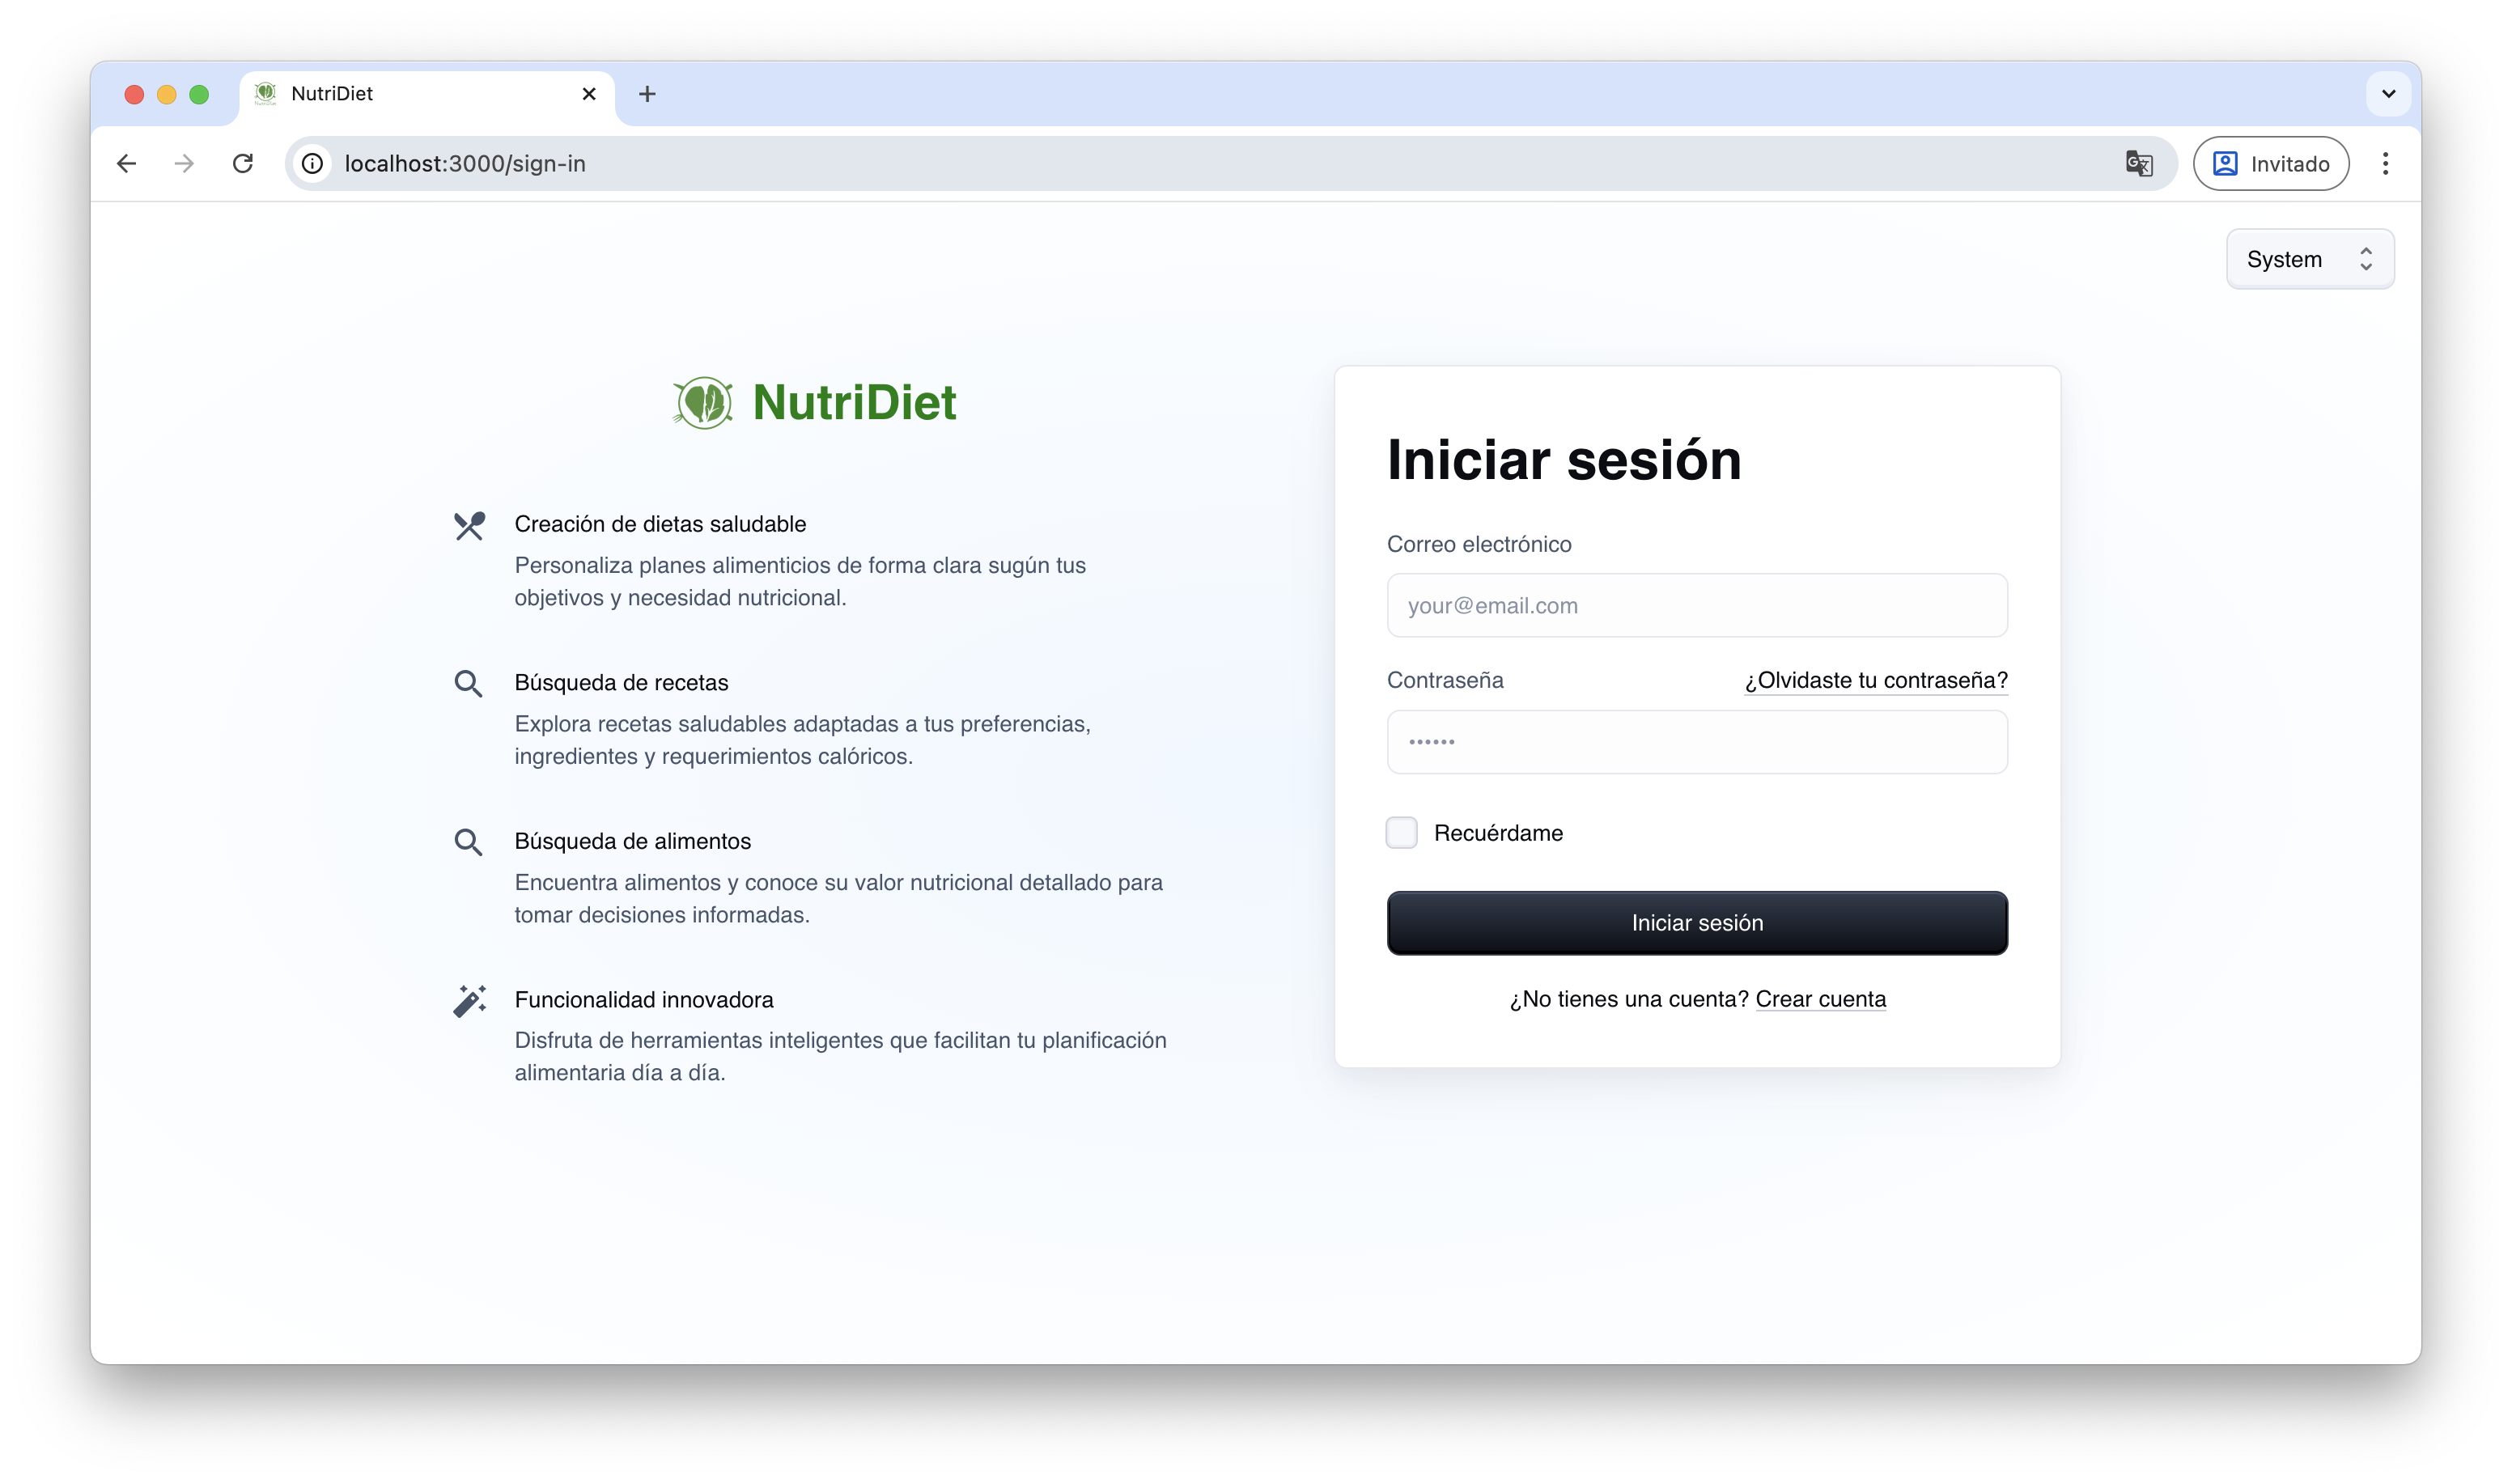
\includegraphics[width=1\linewidth]{Plantilla_TFG_latex//imagenes/Portada_web.png}
    \caption{Portada del sistema}
    \label{fig:Portada_web}
\end{figure}

\subsection{Registro}
Para comenzar a utilizar el sistema, el usuario debe acceder a la opción de registro (Crear cuenta, Figura~\ref{fig:Portada_web_registro}) y completar un formulario con su nombre completo, dirección de correo electrónico y una contraseña segura. Este paso es obligatorio para poder acceder a las funcionalidades del sistema.
\begin{figure}[H]
    \centering
    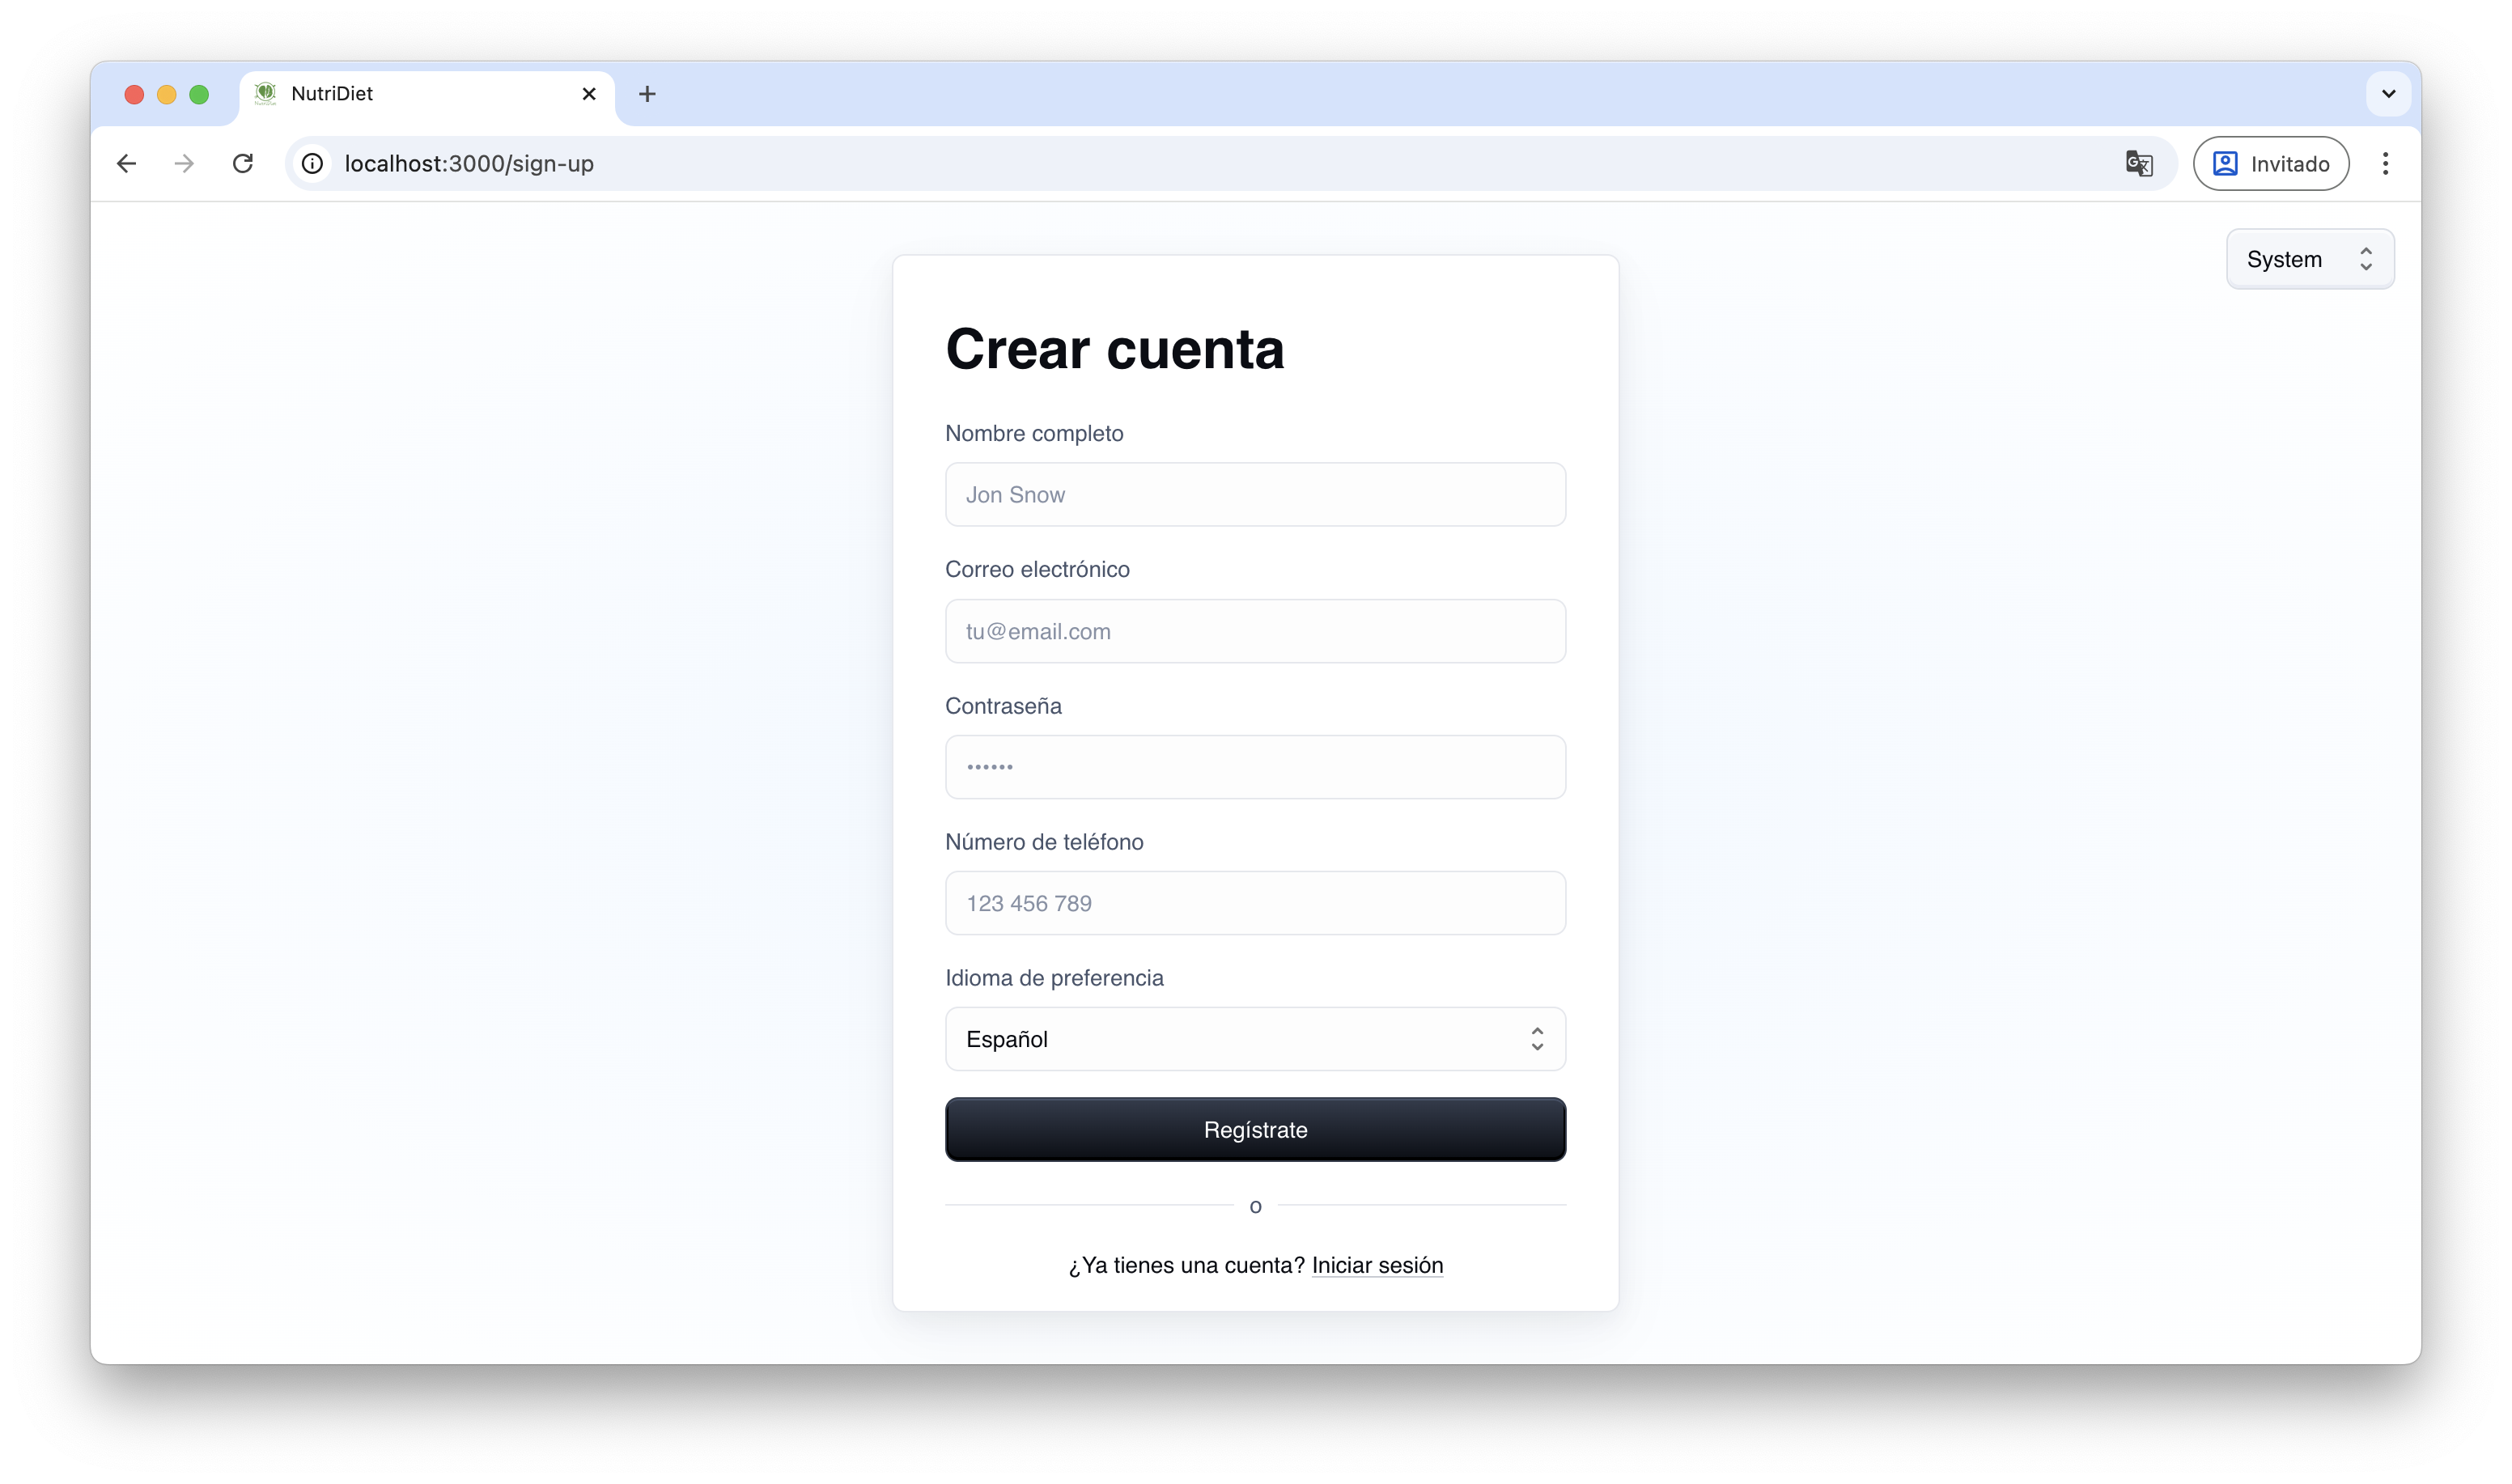
\includegraphics[width=1\linewidth]{Plantilla_TFG_latex//imagenes/Portada_web_registro.png}
    \caption{Tarjeta del registro}
    \label{fig:Portada_web_registro}
\end{figure}

\subsection{Inicio de sesión}
Una vez registrado, el usuario podrá iniciar sesión desde la pantalla principal ingresando su correo electrónico y contraseña. Si ha activado la opción de ``Recordar sesión", el sistema mantendrá su autenticación activa durante un periodo prolongado.

\subsection{Recuperación de contraseña}
En caso de olvidar la contraseña, el sistema dispone de un enlace para iniciar el proceso de recuperación mediante correo electrónico (Figura~\ref{fig:Portada_web_OContrasena}). No obstante, en esta versión, dicha funcionalidad está aún pendiente de implementación, por lo que se recomienda al usuario mantener sus credenciales a buen recaudo.
\begin{figure}[t]
    \centering
    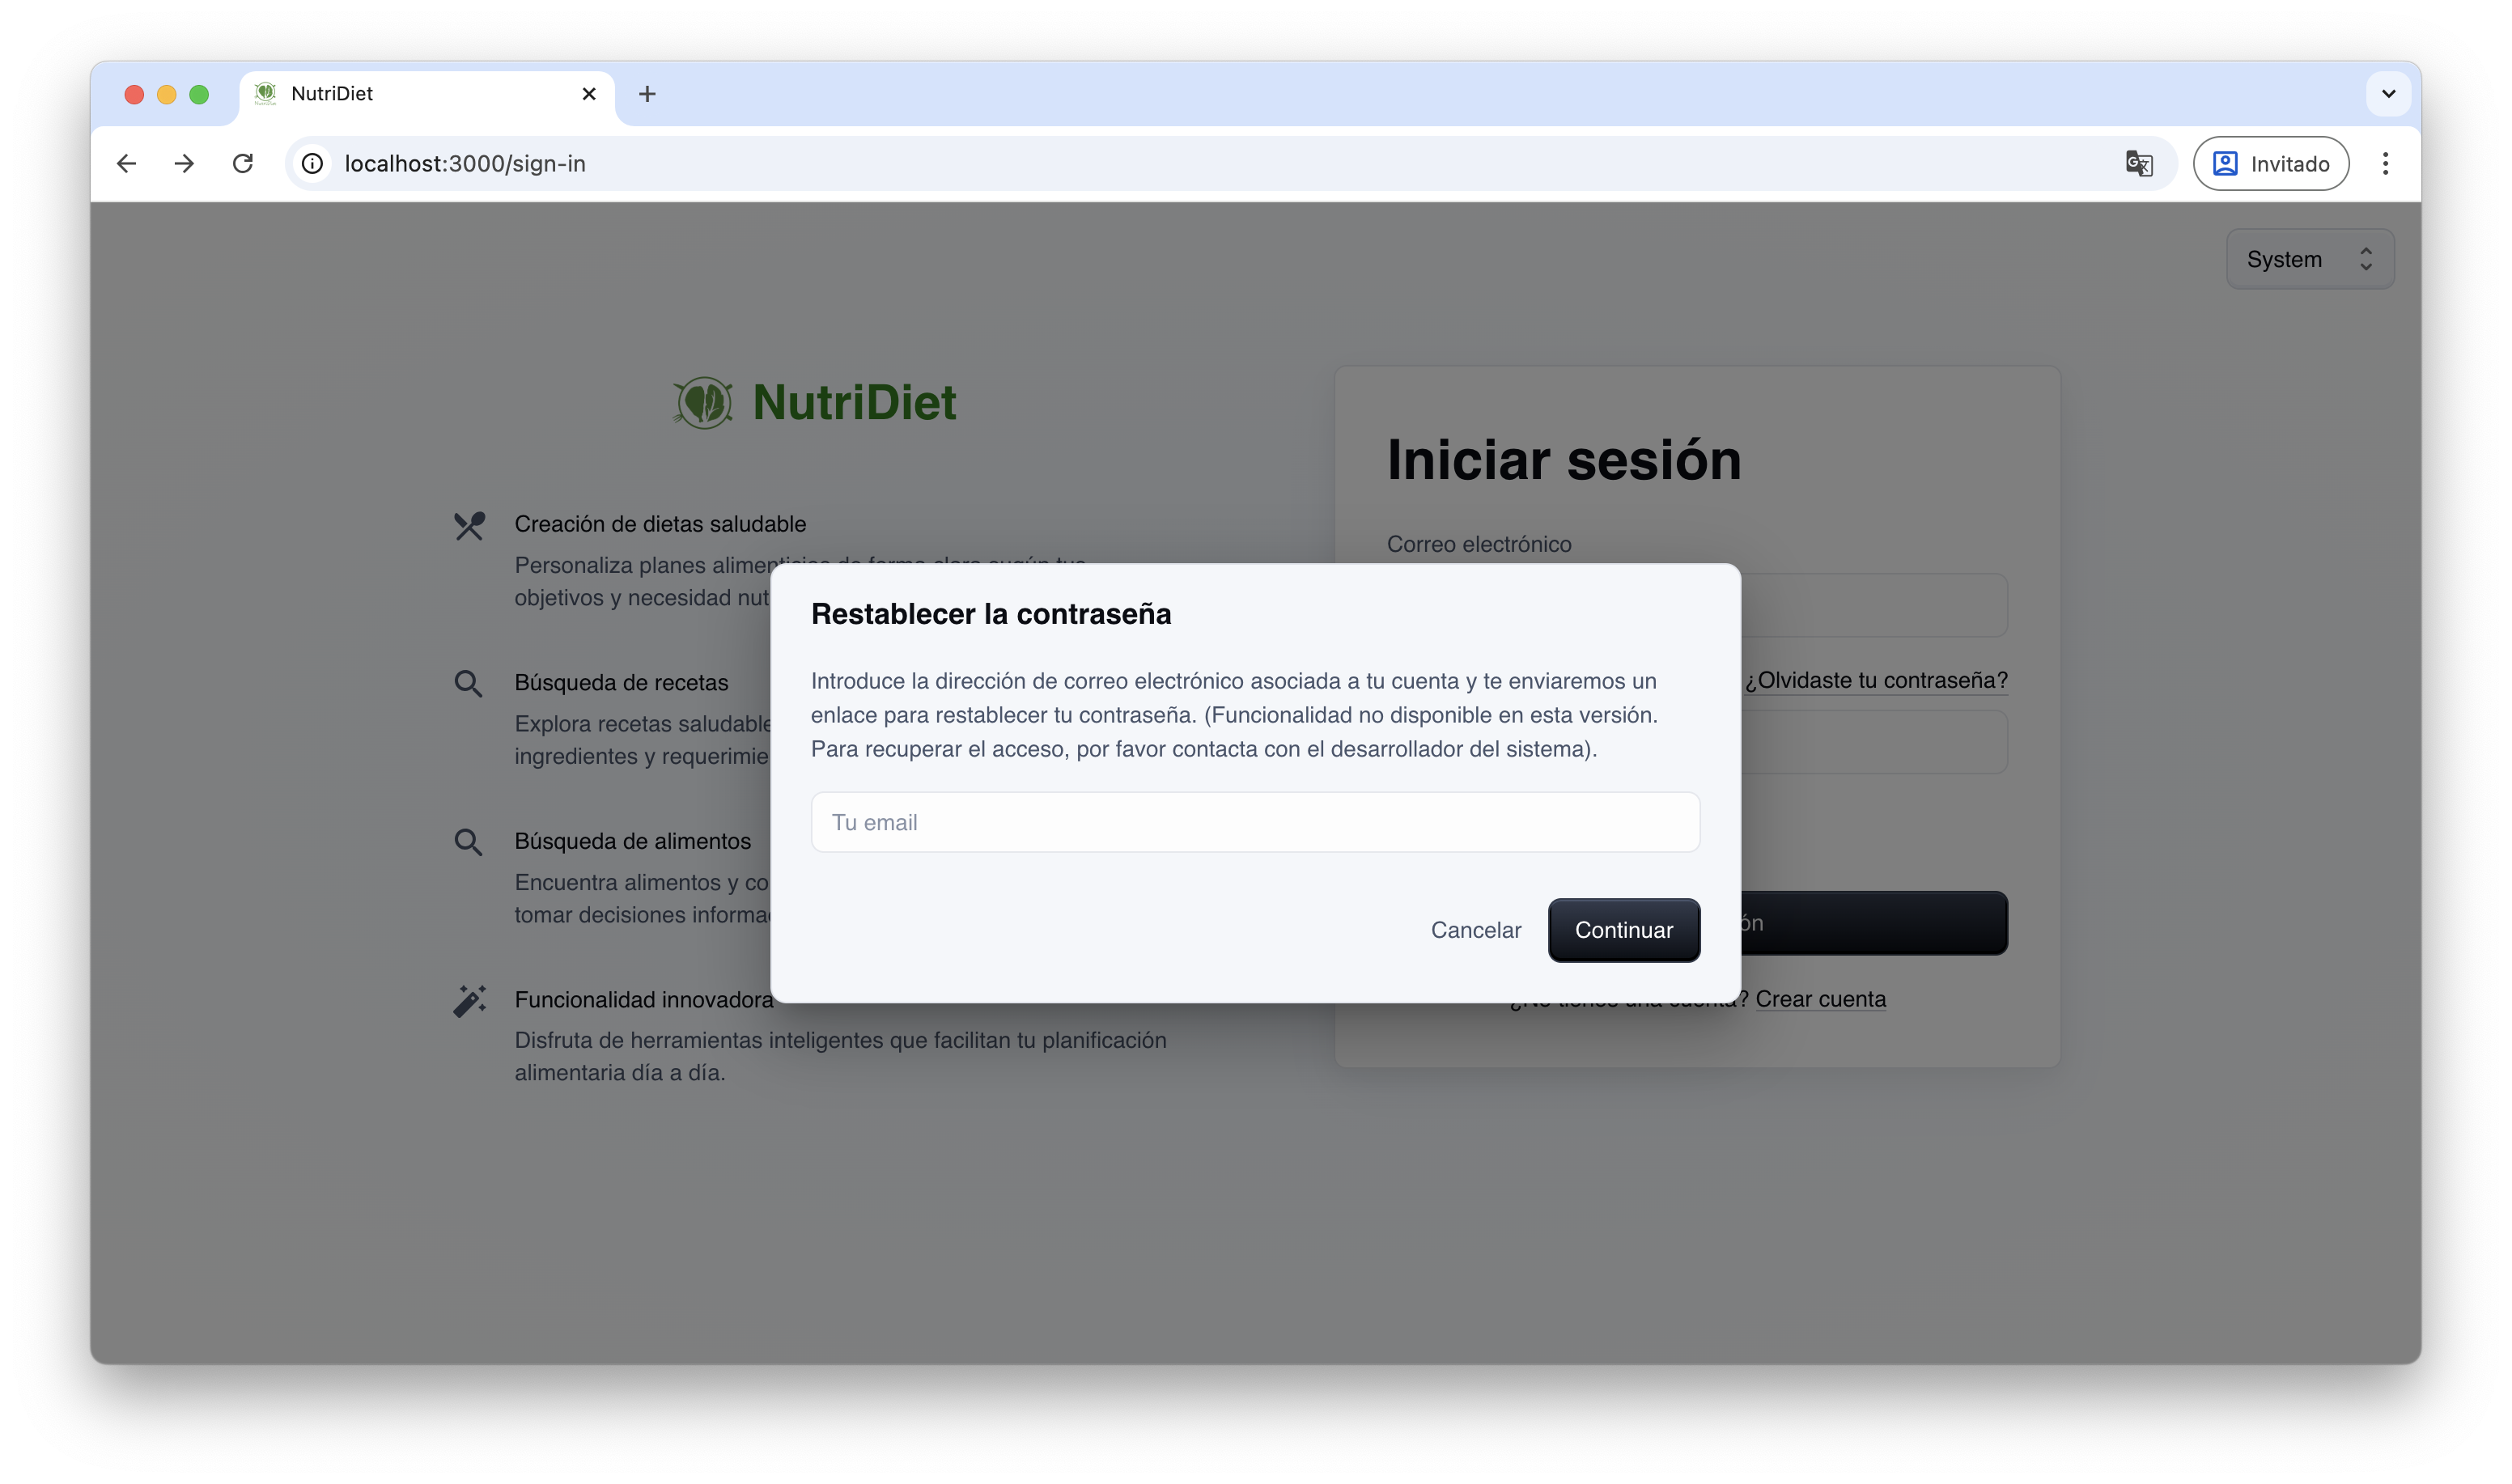
\includegraphics[width=1\linewidth]{Plantilla_TFG_latex//imagenes/Portada_web_OContrasena.png}
    \caption{Tarjeta de recuperación de contraseña}
    \label{fig:Portada_web_OContrasena}
\end{figure}

\section{Página de inicio}
La página de inicio (Figura~\ref{fig:pagina_inicio}) del sistema representa el primer punto de contacto para el usuario tras iniciar sesión. Desde esta interfaz se ofrece una visión general de las funcionalidades disponibles y se proporciona acceso rápido a los módulos principales del sistema.

La estructura de la página de inicio está diseñada para maximizar la usabilidad y facilitar la navegación. Entre sus componentes se encuentran:

\begin{itemize}
    \item Barra de navegación lateral: permite acceder a las secciones clave del sistema, como pacientes, recetas, ingestas y dietas.
    
    \item Cabecera del sistema: contiene un rastro de navegación (``breadcrumb''), el perfil del usuario, representado mediante un avatar generado dinámicamente, y un menú de opciones desplegable accesible desde dicho avatar.

    \item Tarjetas informativas: destacan las funcionalidades principales mediante iconos y descripciones breves, como “Crear nueva dieta”, “Buscar receta” o “Registrar paciente”.
    
\end{itemize}

\begin{figure}[t]
    \centering
    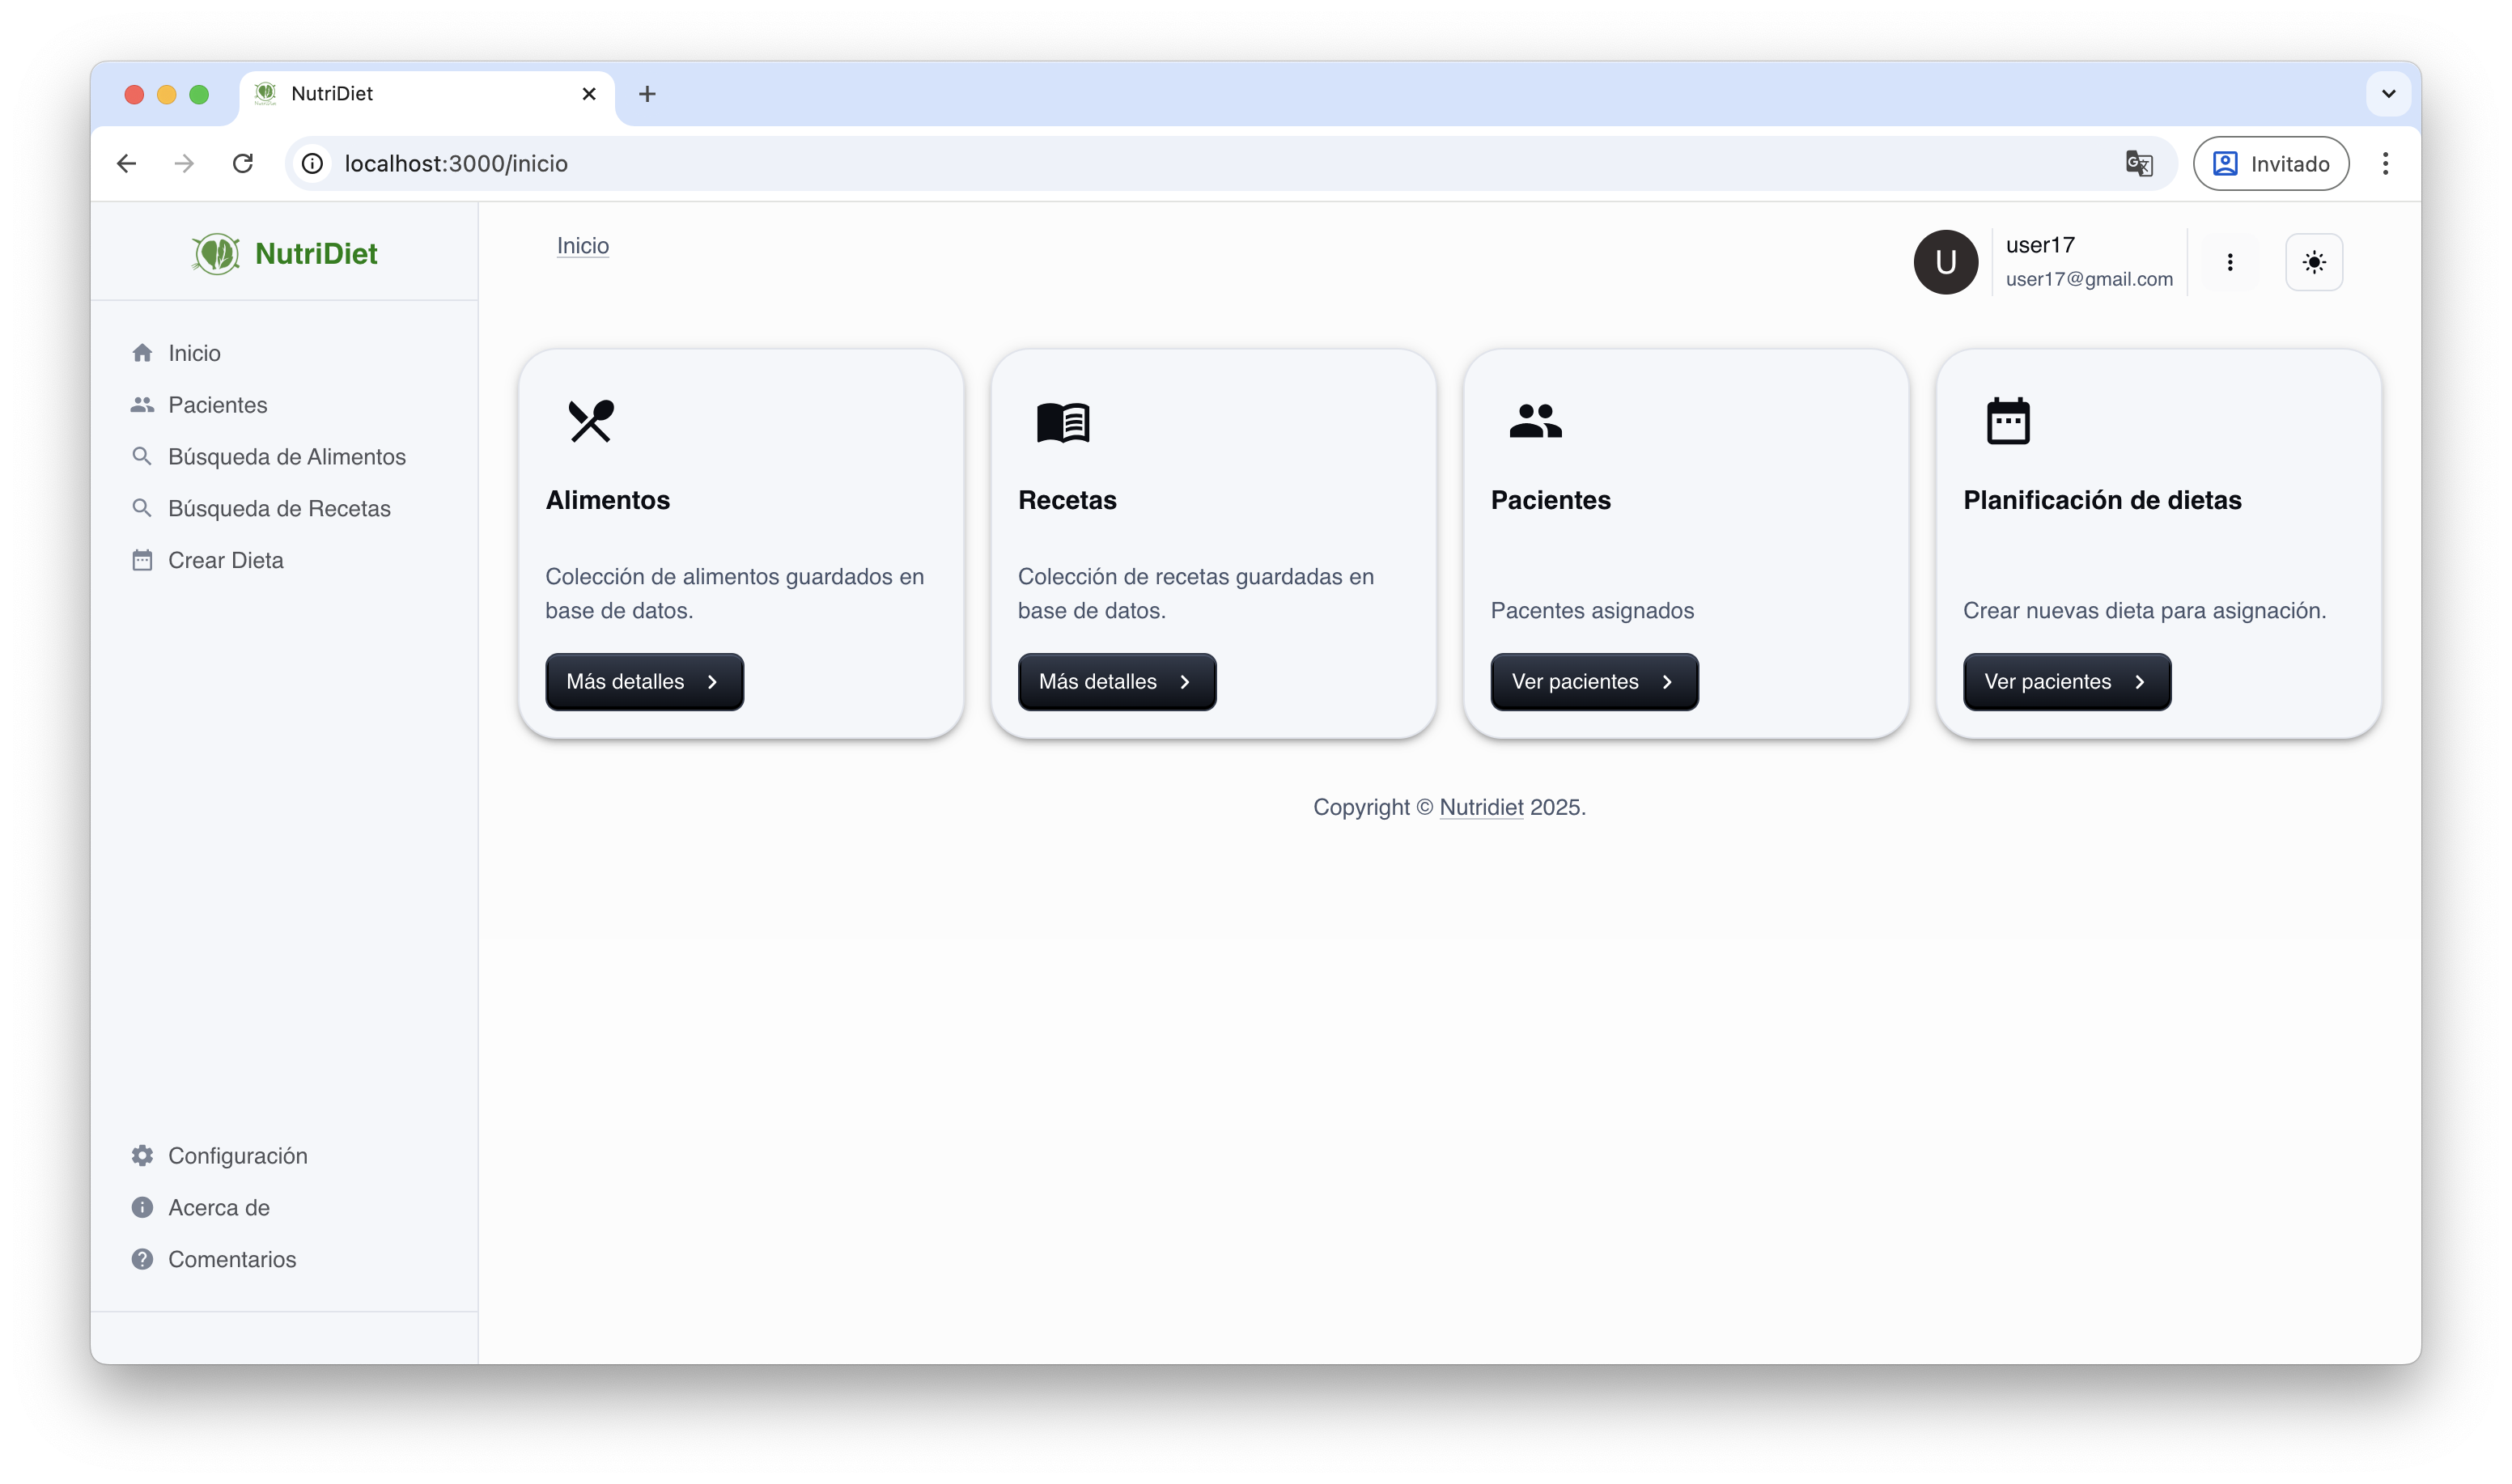
\includegraphics[width=1\linewidth]{Plantilla_TFG_latex/imagenes/PagInicio.png}
    \caption{Interfaz de la página de inicio tras iniciar sesión}
    \label{fig:pagina_inicio}
\end{figure}

\subsection{Menú de opciones del Usuario}
Muestra un avatar generado automáticamente a partir de las iniciales del nombre del usuario, acompañado por su nombre completo y dirección de correo electrónico (Figura~\ref{fig:PagInicio_menuO}). Al hacer clic en el icono de tres puntos junto al avatar, se despliega un menú de opciones que permite realizar acciones como acceder al perfil, modificar configuraciones de la cuenta o cerrar sesión.
\begin{figure}
    \centering
    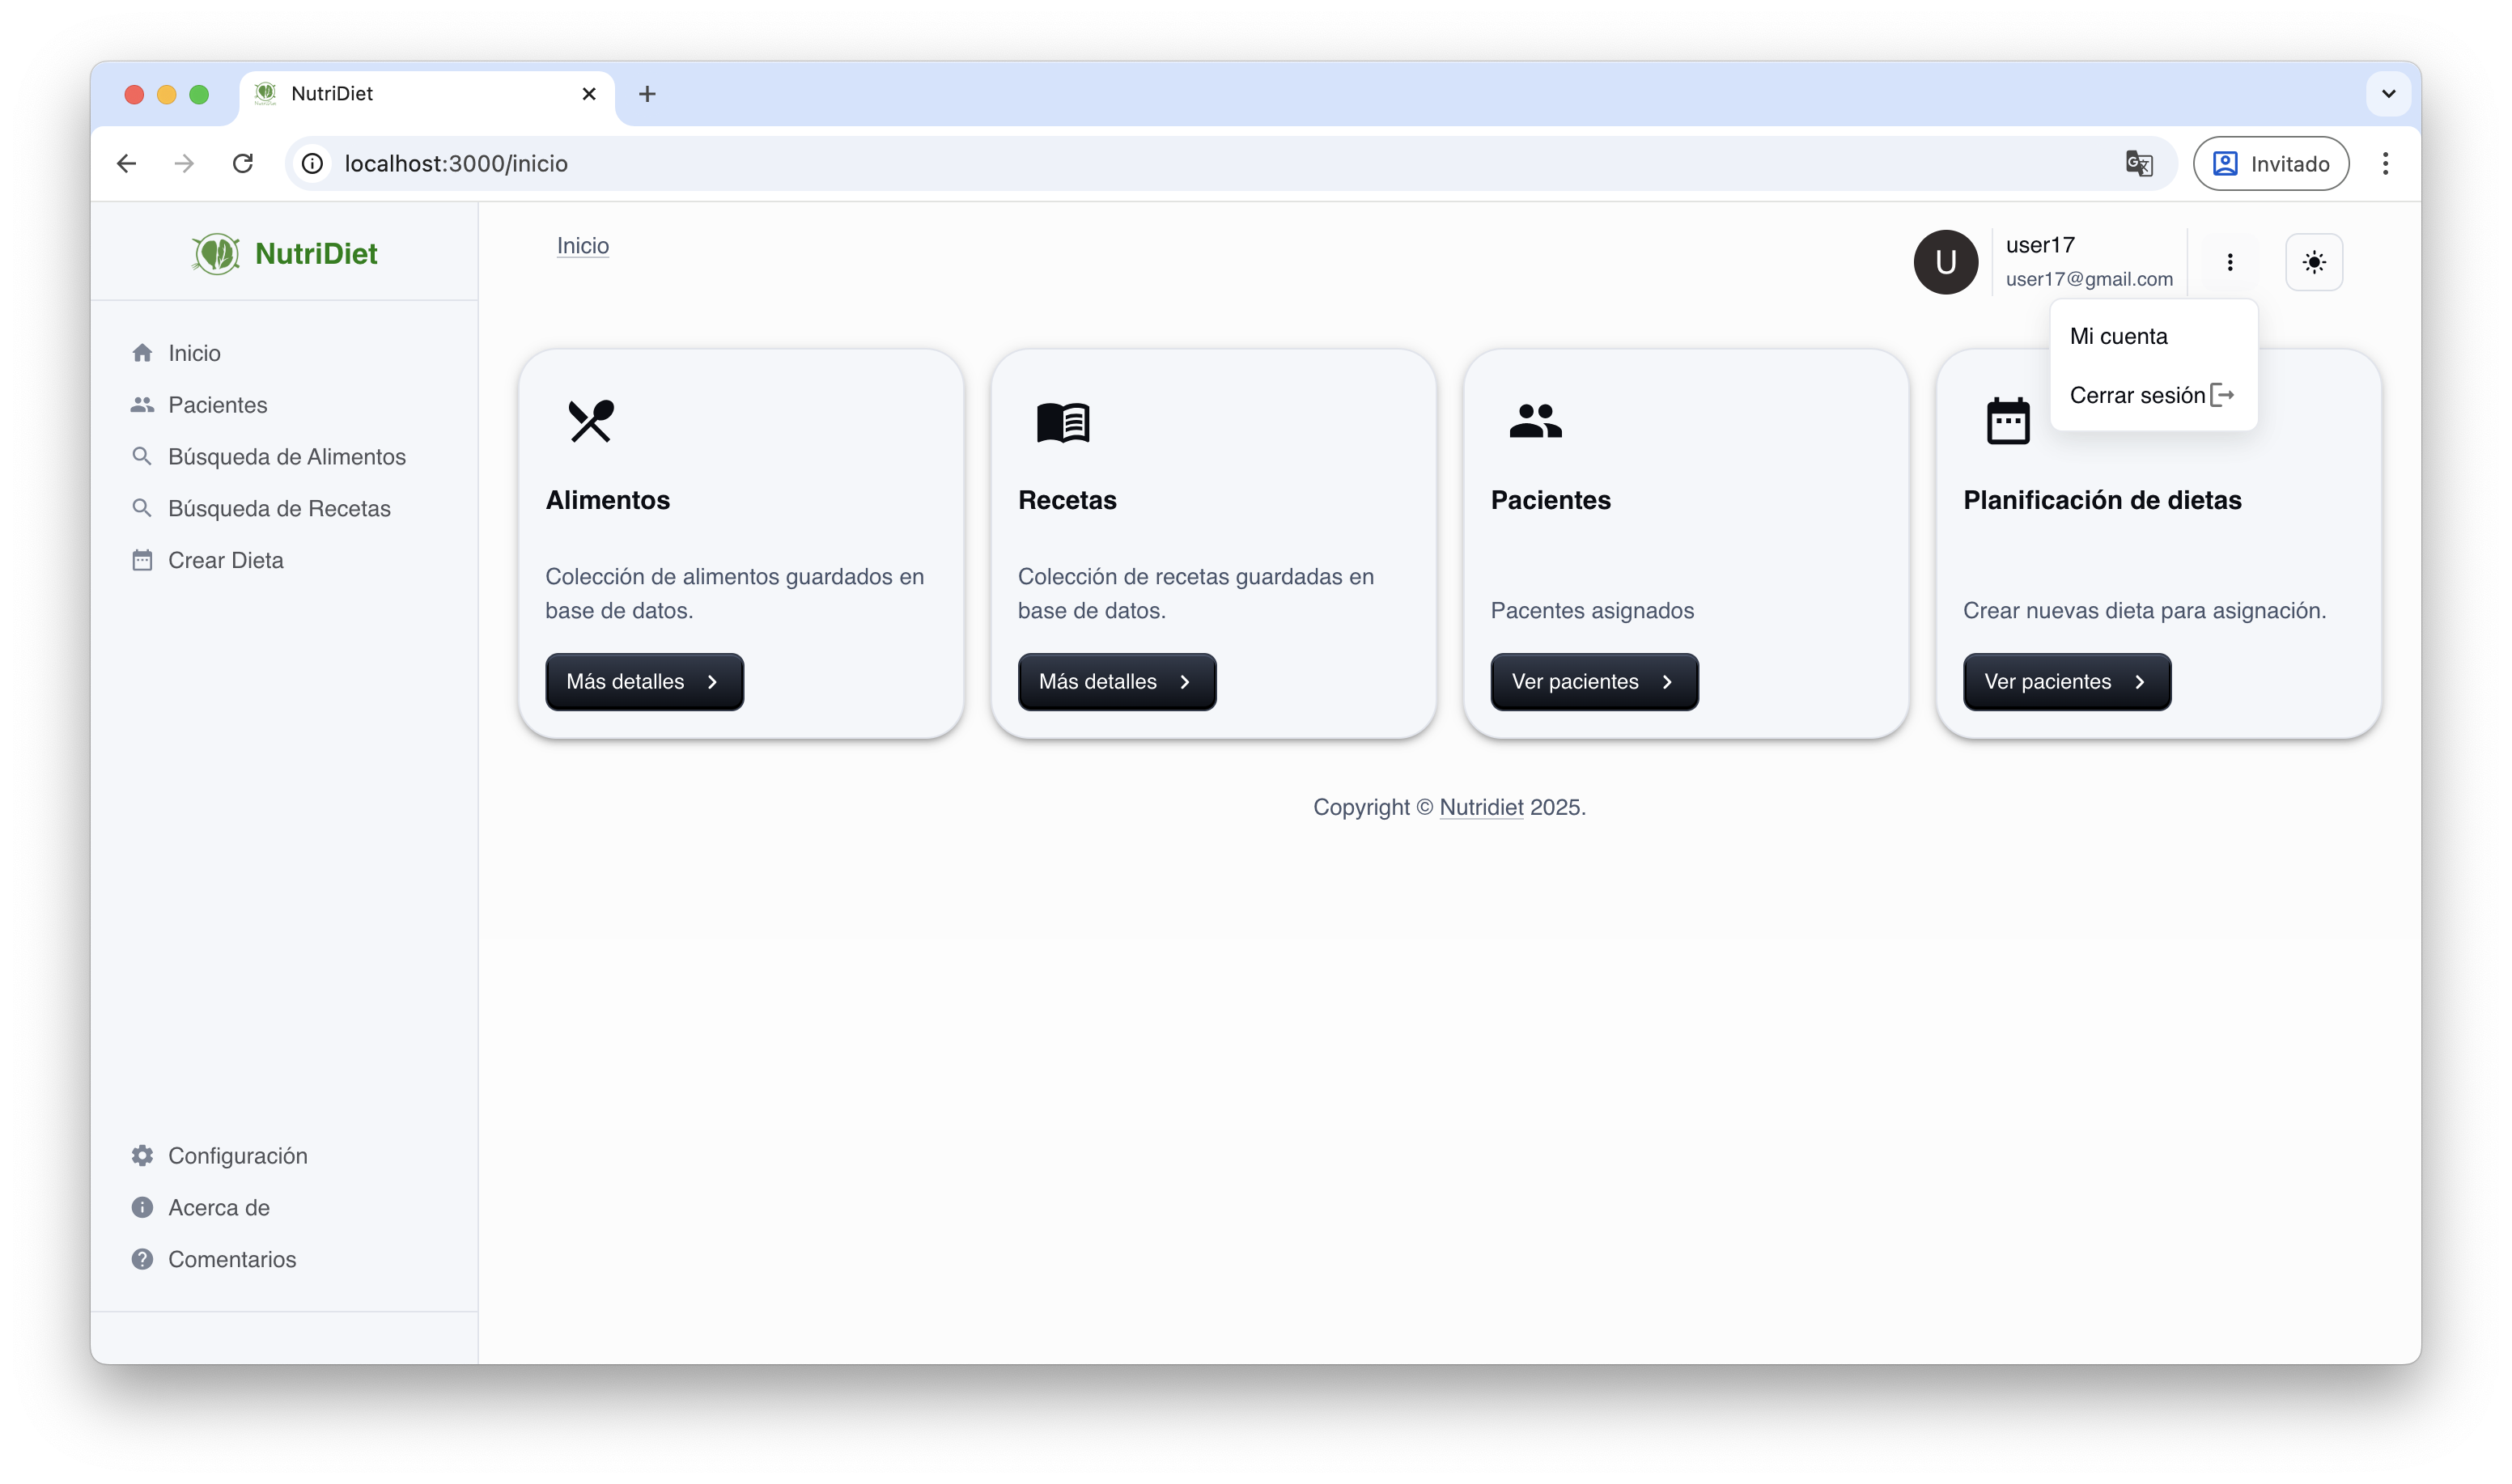
\includegraphics[width=1\linewidth]{Plantilla_TFG_latex/imagenes/PagInicio_OM.png}
    \caption{Menú de opciones del Usuario}
    \label{fig:PagInicio_menuO}
\end{figure}

\subsubsection{Mi cuenta}
Esta página (Figura~\ref{fig:PagInicio_MiCuenta}) permite al usuario gestionar y actualizar su información personal de forma segura. El usuario puede modificar datos como el nombre completo, el número de teléfono y el idioma de preferencias.

Además, se incluye una opción para cambiar la contraseña, lo que refuerza la seguridad y permite mantener actualizadas las credenciales de acceso.

\begin{figure}
    \centering
    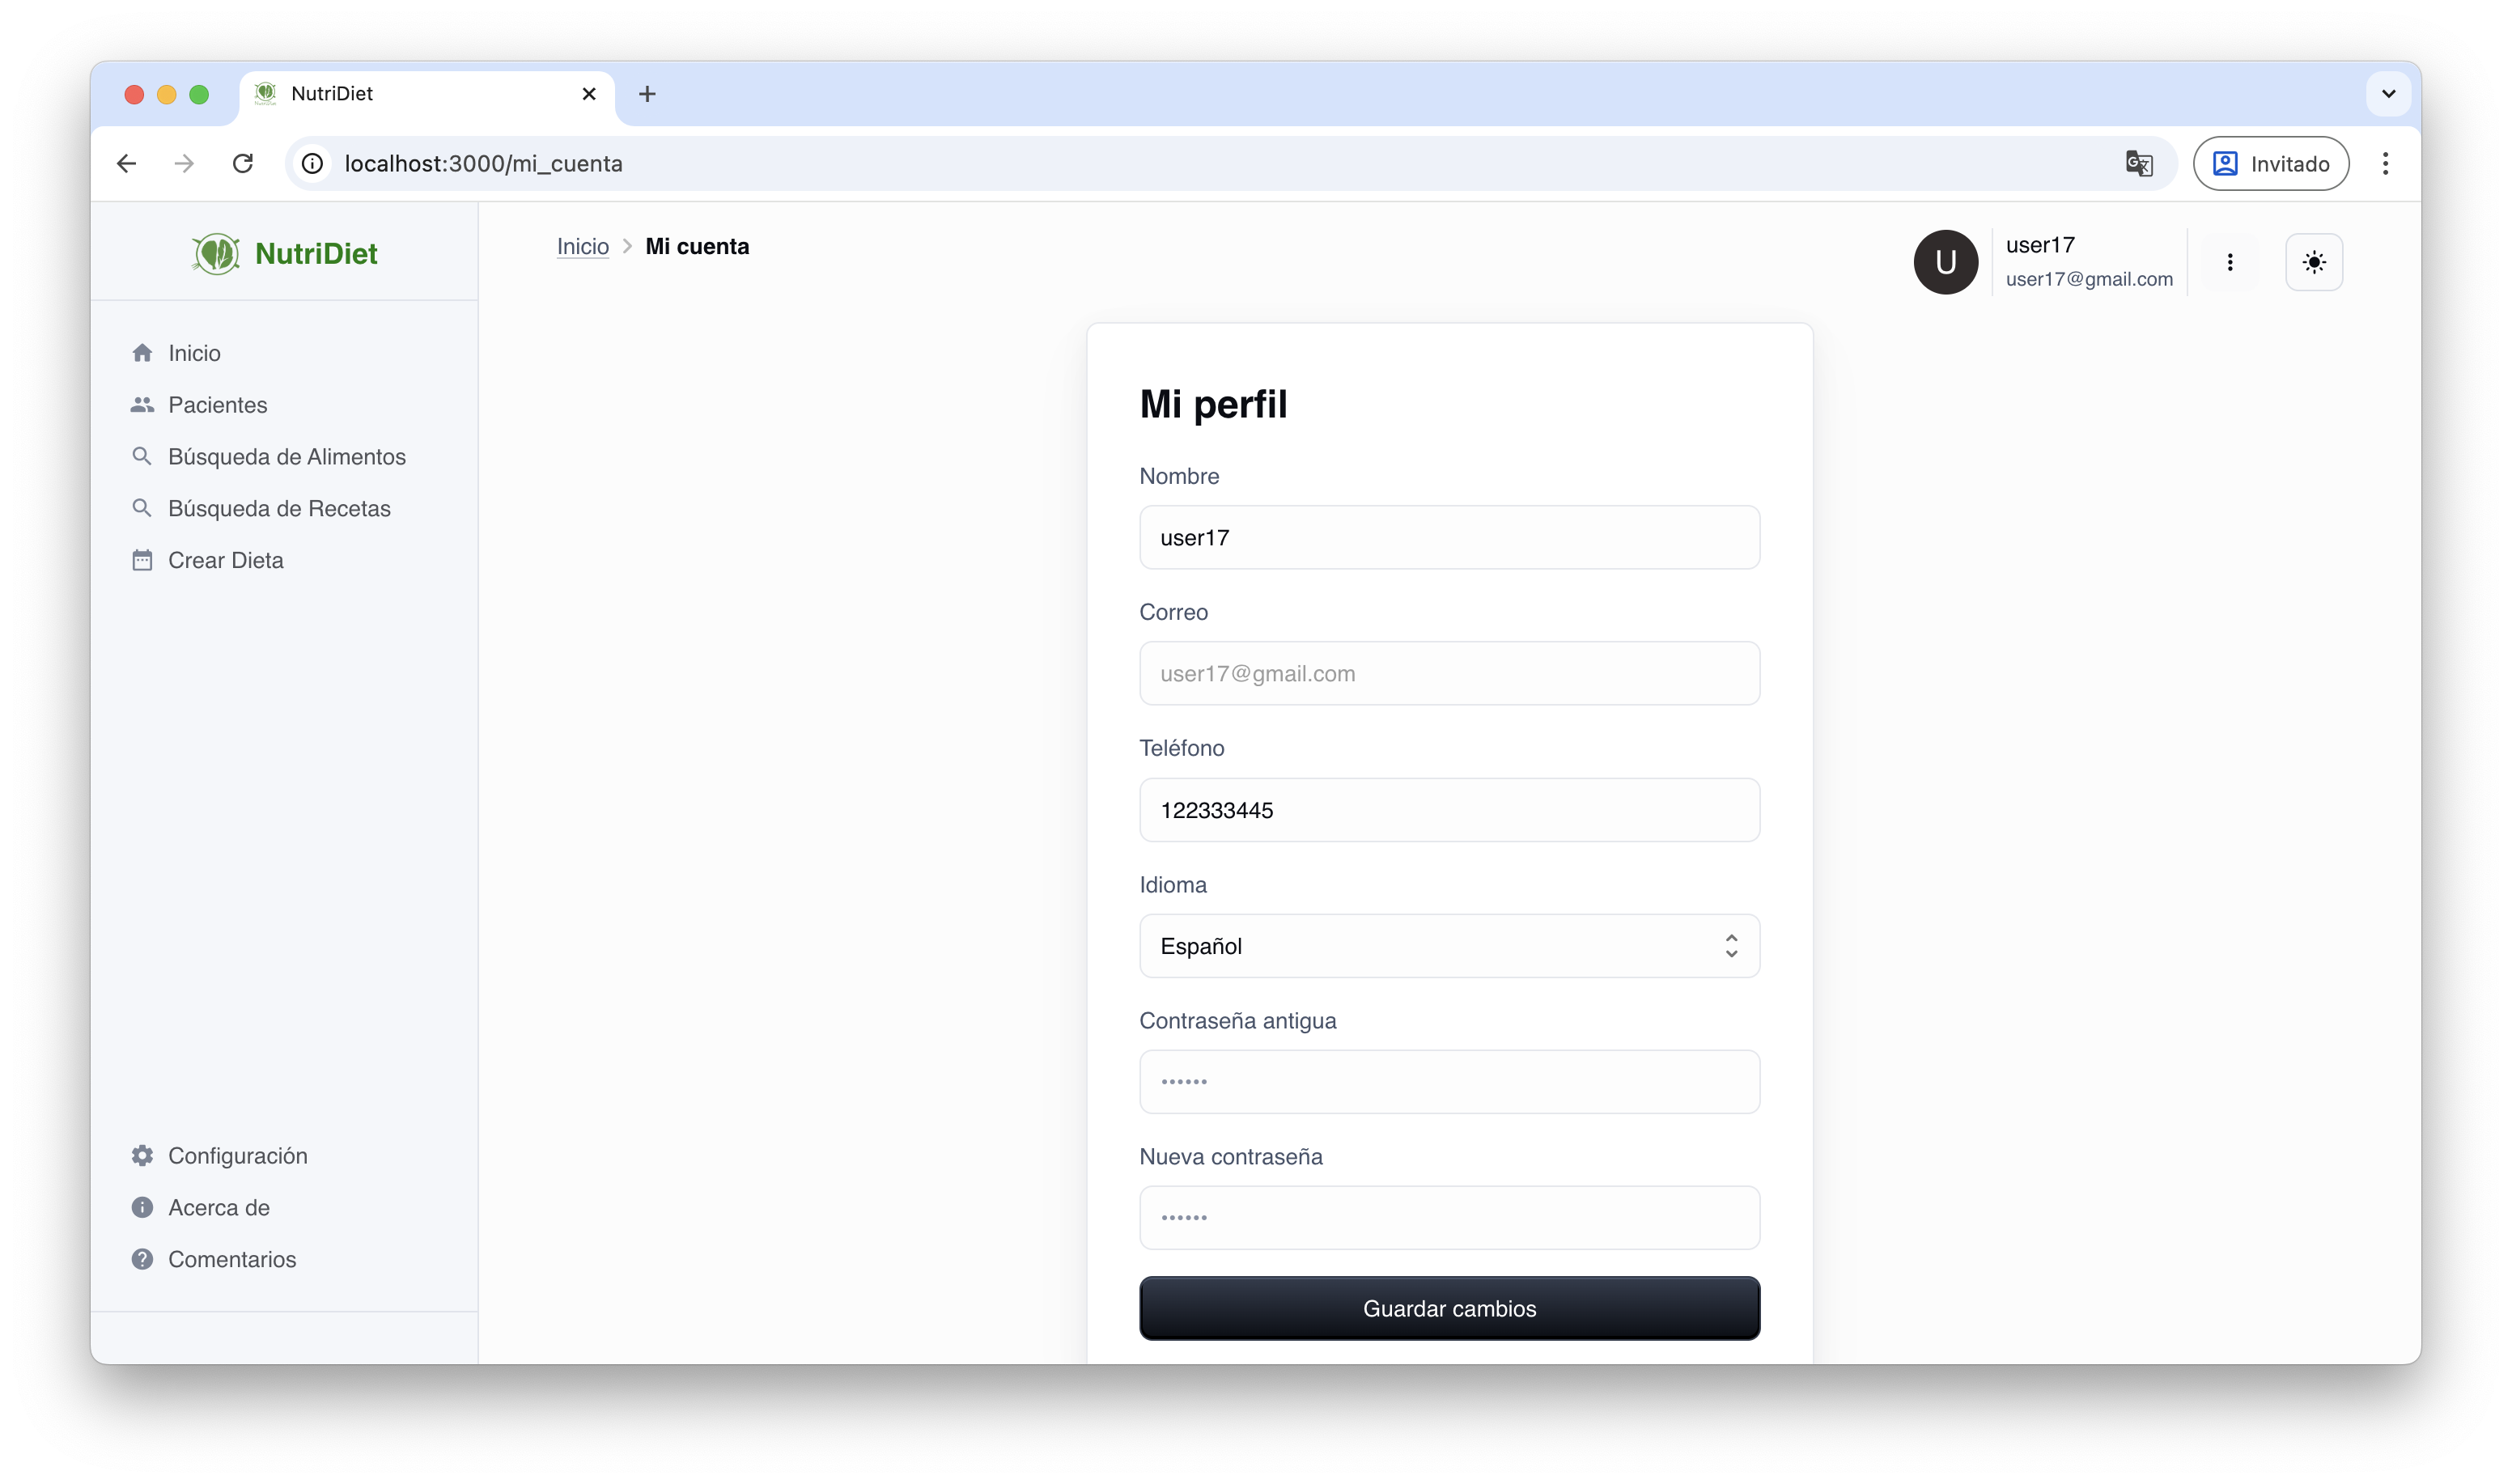
\includegraphics[width=1\linewidth]{Plantilla_TFG_latex/imagenes/PagInicio_MiCuenta.png}
    \caption{Vista de gestión de cuenta del usuario}
    \label{fig:PagInicio_MiCuenta}
\end{figure}

\subsubsection{Cerrar sesión}

El sistema permite al usuario cerrar sesión de forma segura mediante el menú de opciones accesible desde el avatar situado en la cabecera. Al seleccionar la opción Cerrar sesión, la sesión actual se finaliza y el usuario es redirigido automáticamente a la portada del sistema, donde podrá iniciar sesión nuevamente o registrar una nueva cuenta.

\section{Gestión de pacientes}

La sección de gestión de pacientes (Figura~\ref{fig:PagPaciente_ini}) permite al usuario registrar, visualizar, editar y eliminar pacientes asociados a su cuenta profesional. Se ha diseñado teniendo en cuenta que la aplicación está dirigida a personal experto, esta funcionalidad resulta esencial para organizar y personalizar el seguimiento clínico de cada caso.

\begin{itemize}
    \item Añadir paciente: Tarjeta visible en la interfaz principal que permite iniciar el proceso de registro de un nuevo paciente. Al hacer clic, se despliega un formulario de creación.
    
    \item Tarjeta paciente: Tarjeta que representa individualmente a cada paciente. Muestra su información básica y proporciona botones para editar o eliminar al paciente.

    \item Visualización de detalle de dieta: Desde cada tarjeta de paciente, el usuario puede acceder a las dietas previamente asignadas. 
    
    \item Navegación paginada: Si hay más de cinco pacientes, se activa una navegación por páginas, que permite avanzar o retroceder en bloques de cinco registros.
\end{itemize}

\begin{figure}[H]
    \centering
    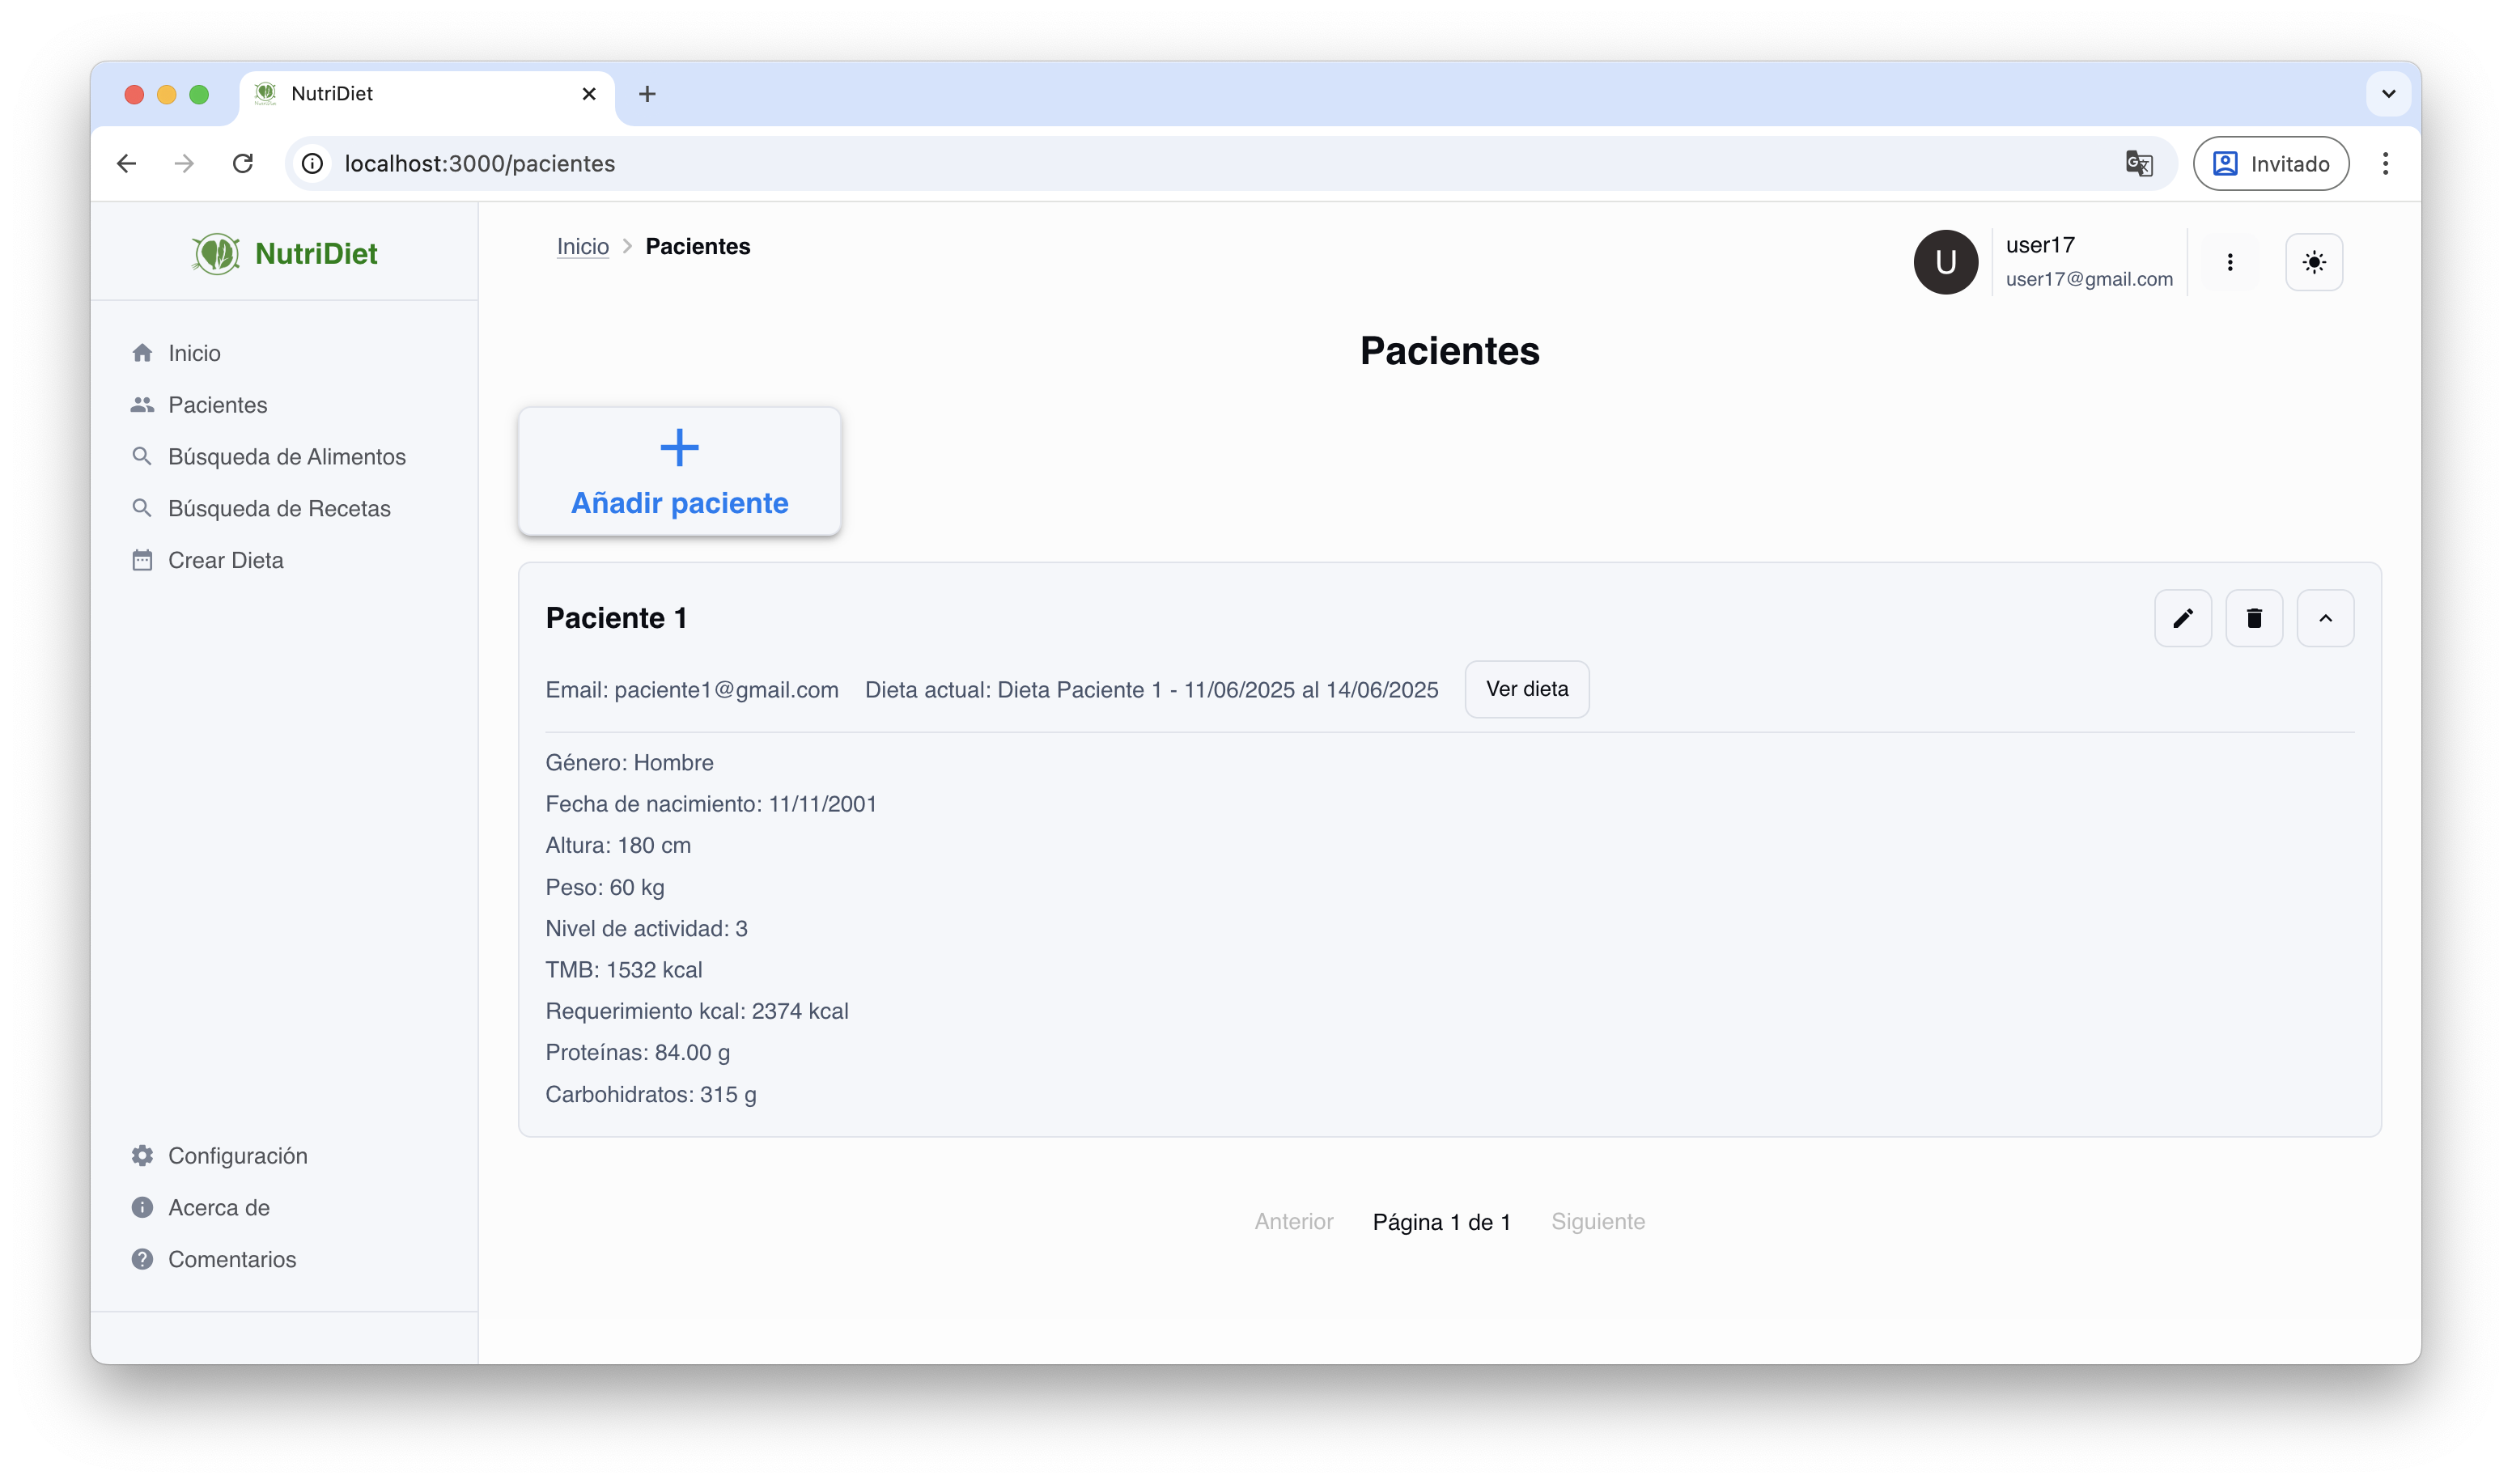
\includegraphics[width=1\linewidth]{Plantilla_TFG_latex/imagenes/PagPaciente_ini.png}
    \caption{Vista de Pacientes}
    \label{fig:PagPaciente_ini}
\end{figure}

\subsection{Añadir paciente}
Para registrar nuevos pacientes se realiza mediante este formulario accesible desde la interfaz principal de la sección Pacientes (Figura~\ref{fig:Paciente_crearP}). Una vez completado el formulario, pulsar el botón ``Guardar'' para registrar al paciente en la base de datos. Al finalizar, el paciente aparecerá automáticamente en el listado general, y podrá ser editado o eliminado posteriormente si es necesario.

\begin{figure}[H]
    \centering
    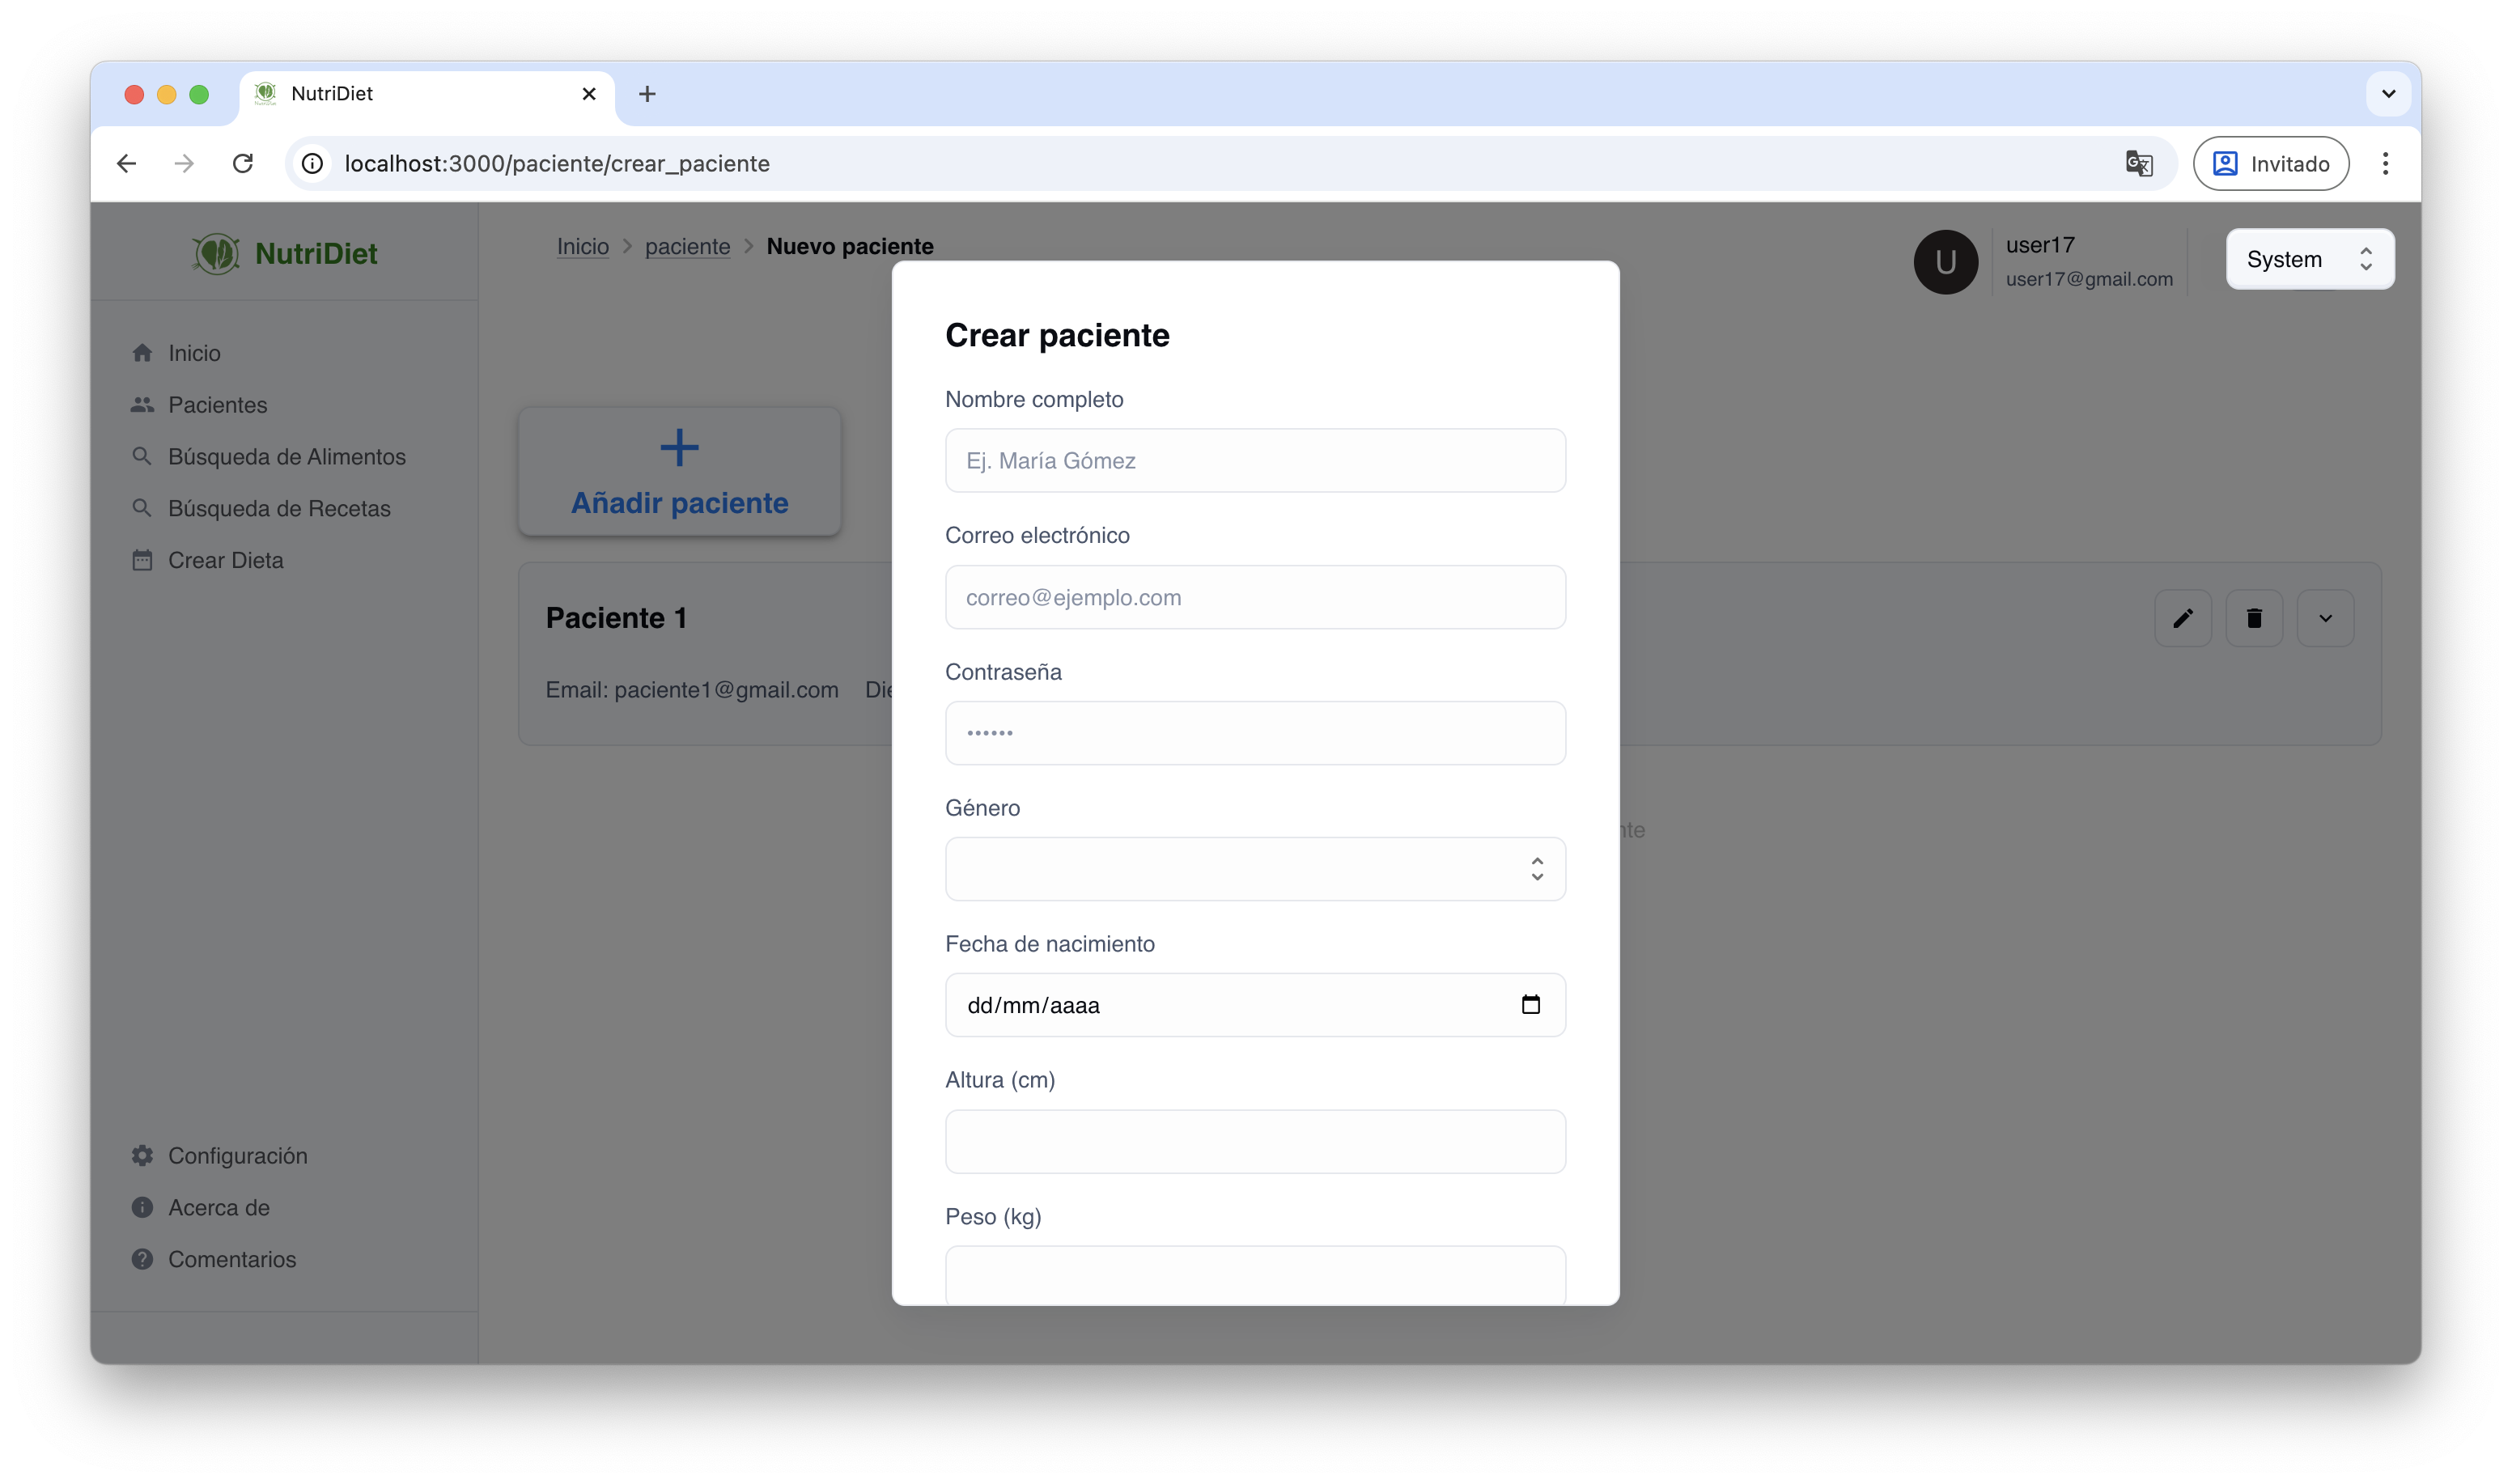
\includegraphics[width=1\linewidth]{Plantilla_TFG_latex//imagenes/Paciente_crearP.png}
    \caption{Formulario de creación de un nuevo paciente}
    \label{fig:Paciente_crearP}
\end{figure}

\subsection{Visualización detallada de dietas}
Mediante el botón ``Ver dieta'', el usuario puede acceder al detalle completo de una dieta asignada a un paciente. Esta vista muestra el nombre de la dieta, el periodo de validez, el nombre del paciente y el nutricionista responsable (Figura~\ref{fig:detalle_dieta_visual}). A continuación, se presenta una tabla diaria con las ingestas planificadas, donde se agrupan las recetas por tipo (desayuno, almuerzo, cena, etc.) y subtipo (primer plato, bebida, postre, etc.). Para cada receta incluye un botón para acceder a su ficha completa. 
\begin{figure}
    \centering
    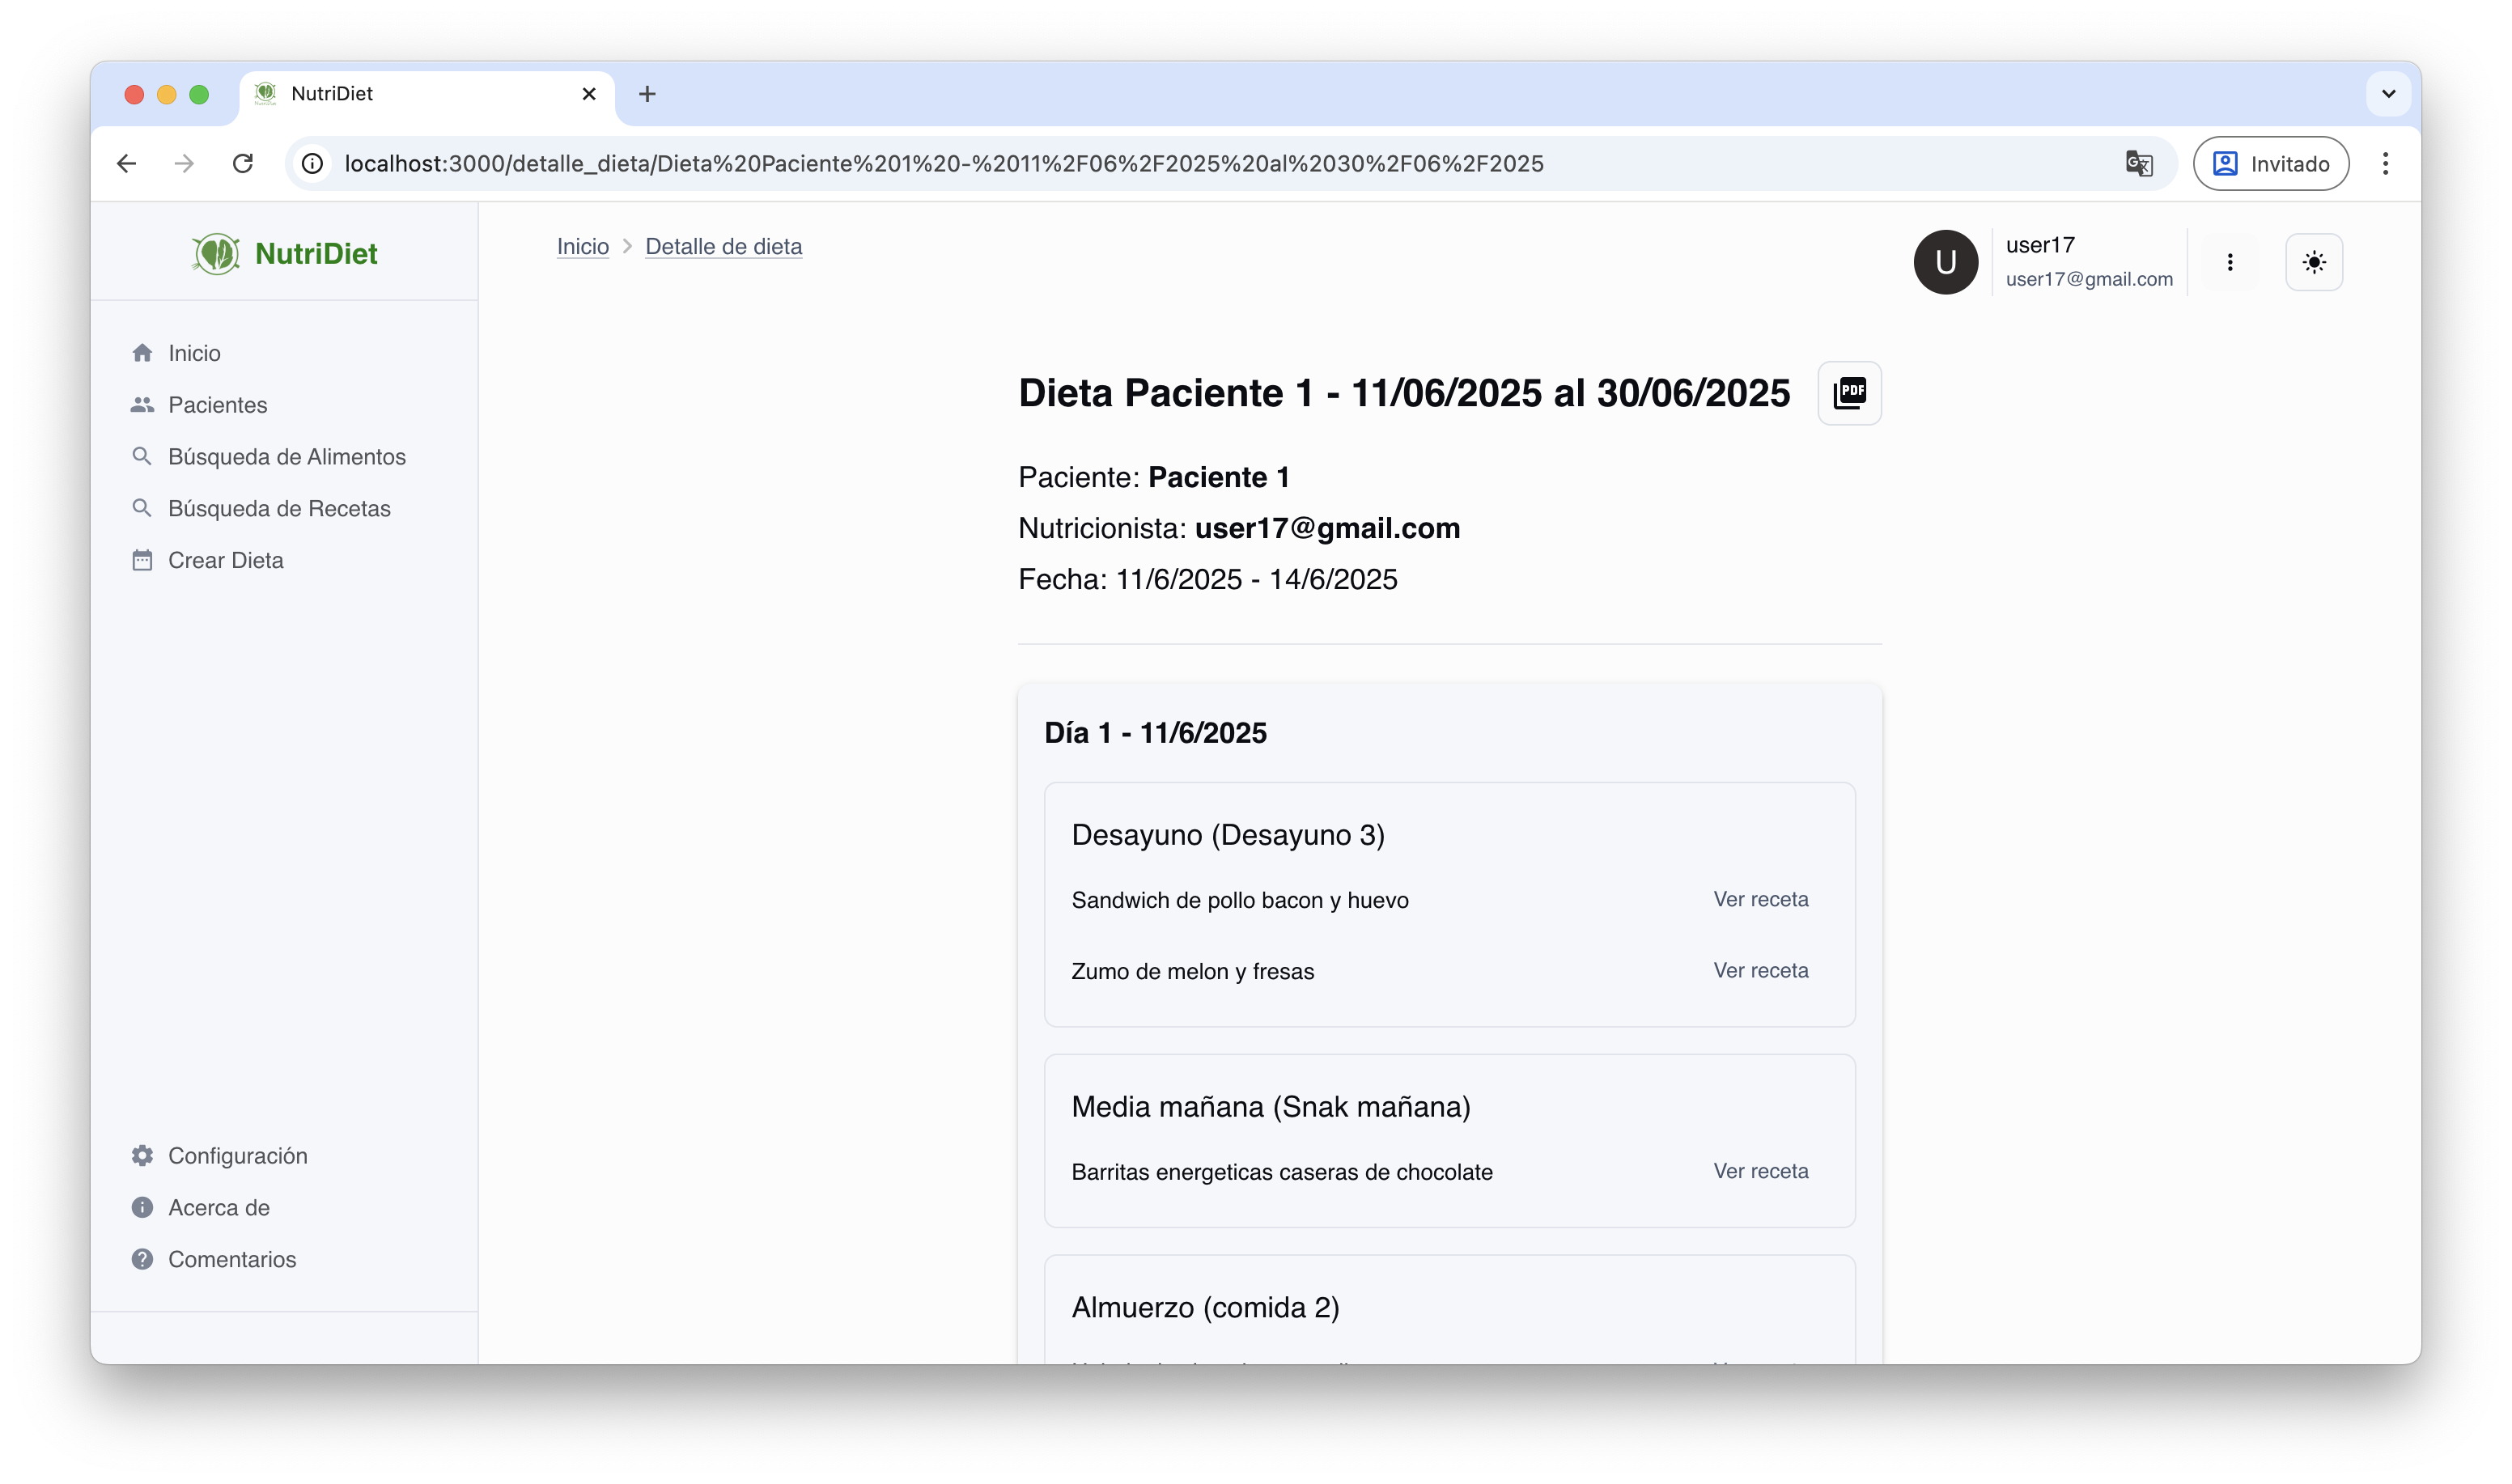
\includegraphics[width=1\linewidth]{Plantilla_TFG_latex/imagenes/PagPaciente_detalleDieta.png}
    \caption{Vista detallada de una dieta asignada a un paciente}
    \label{fig:detalle_dieta_visual}
\end{figure}

\begin{figure}
    \centering
    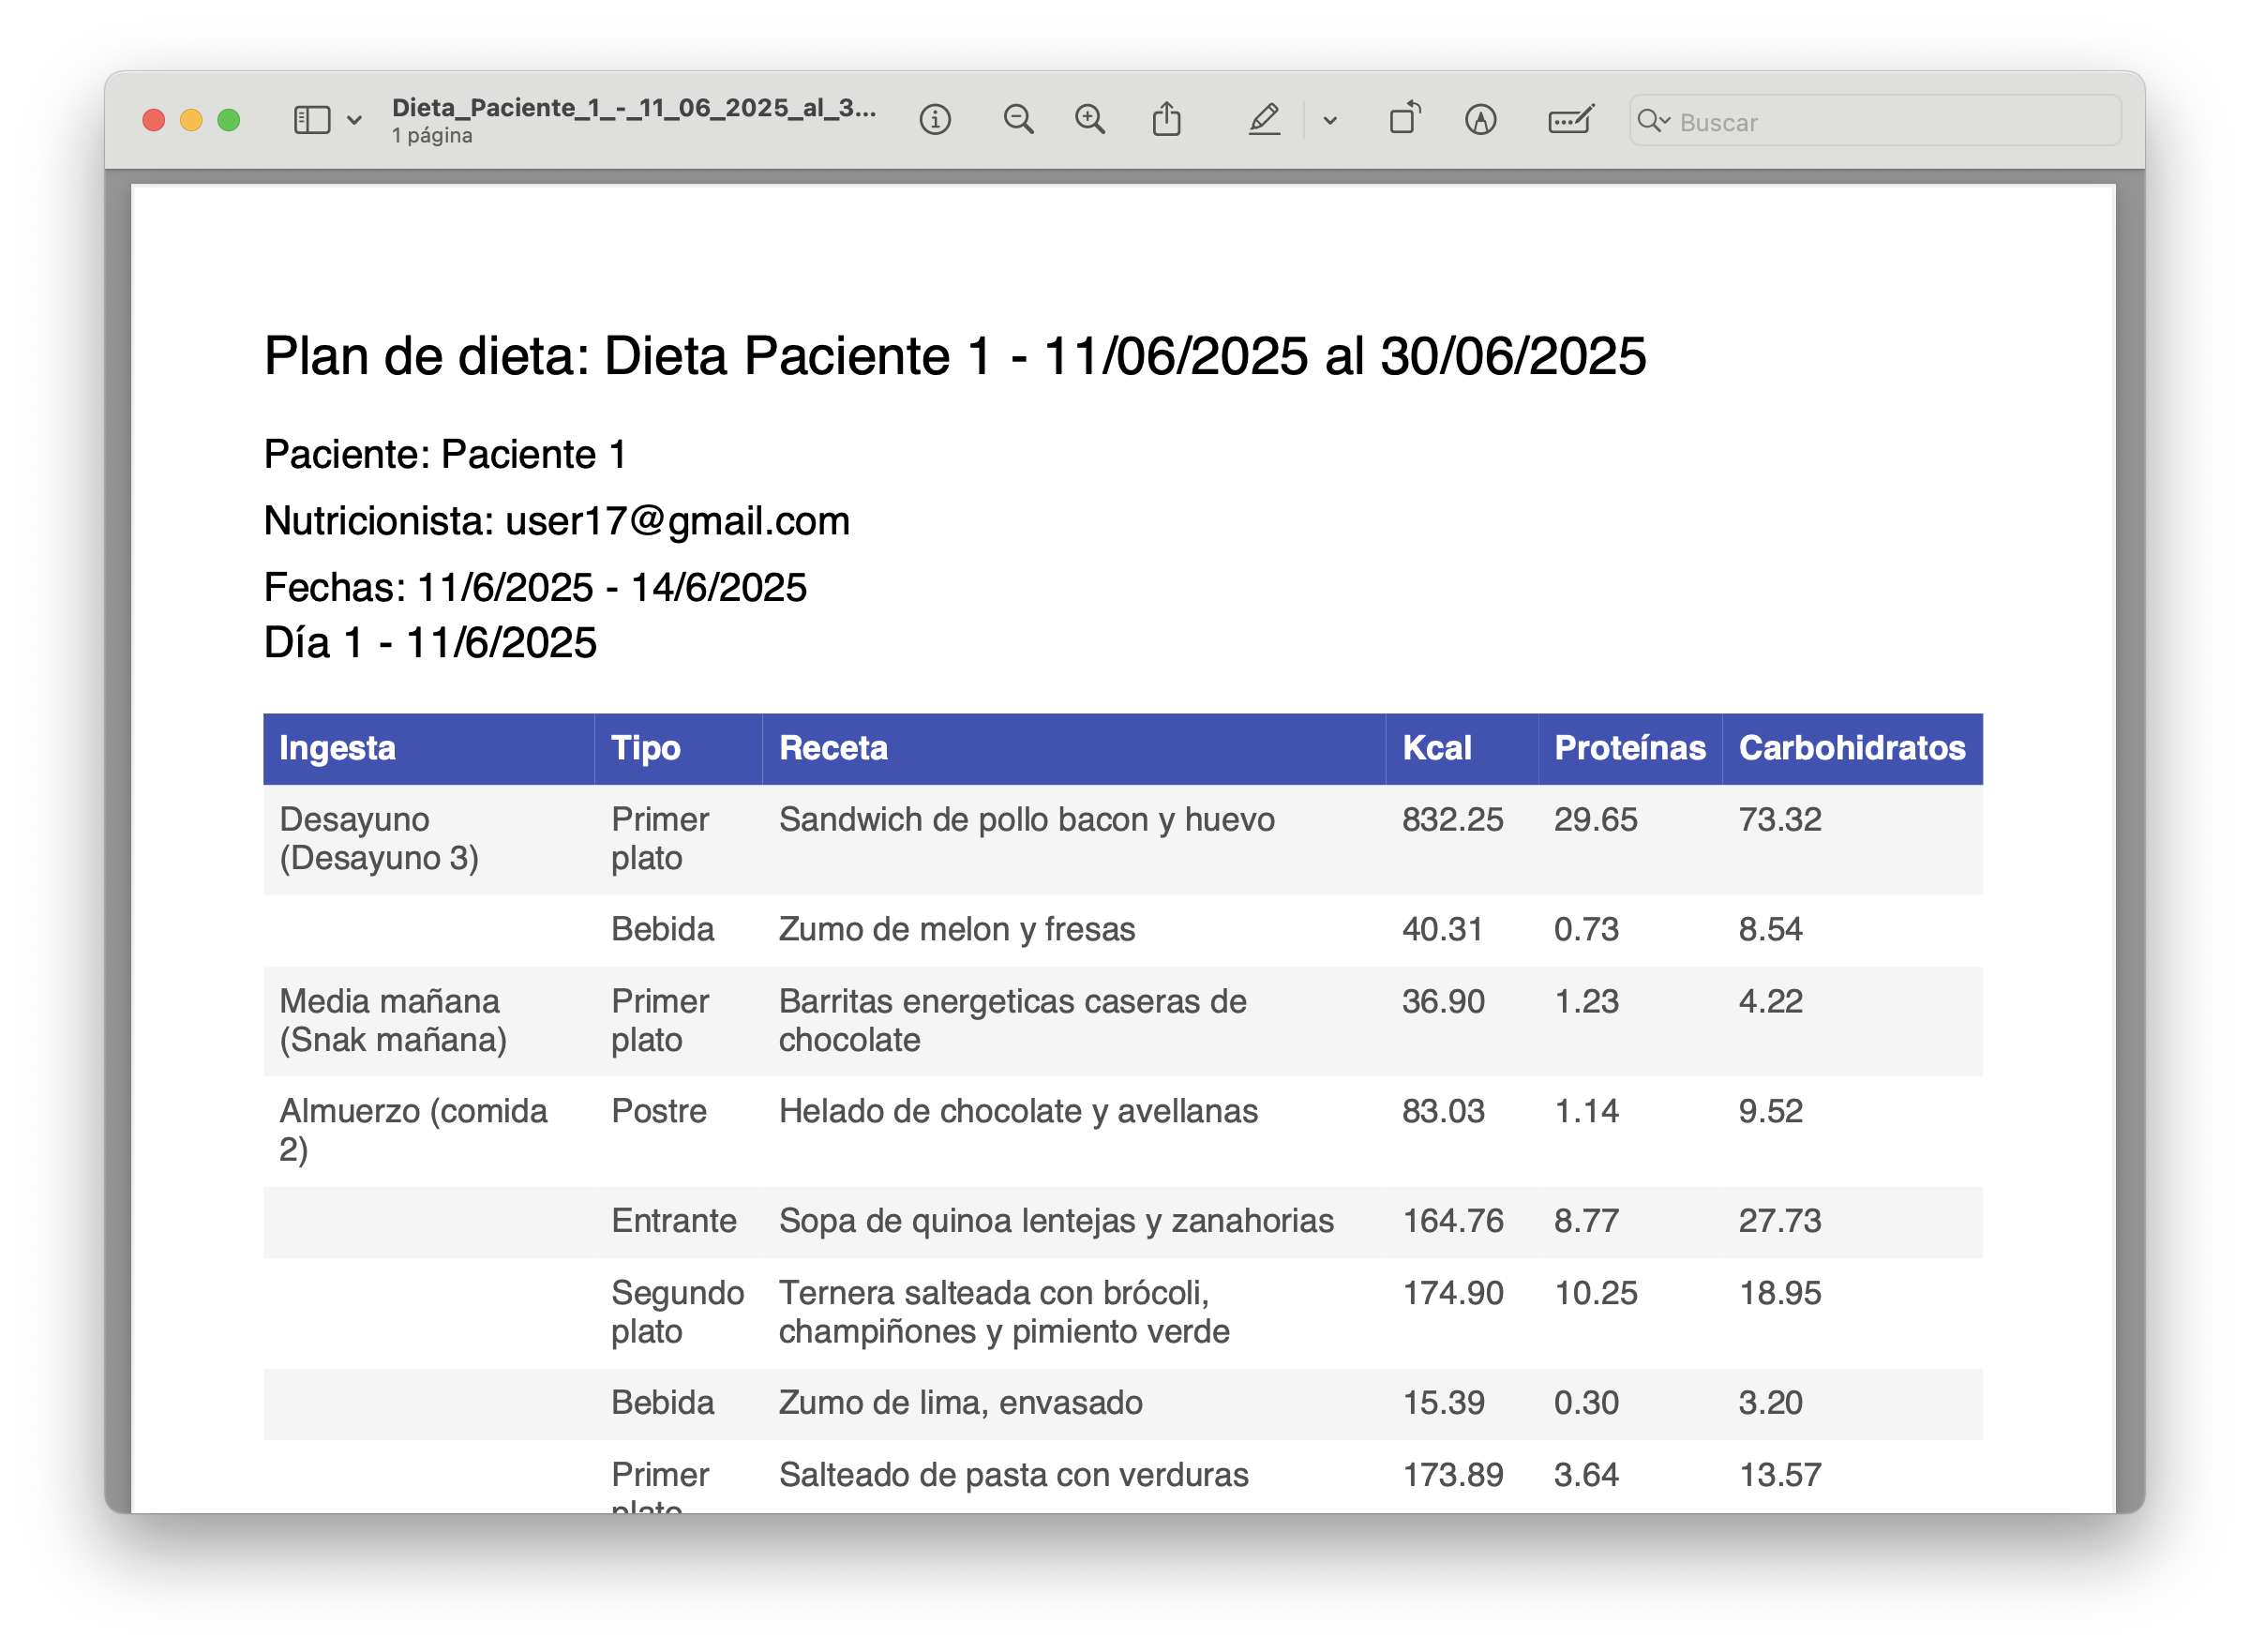
\includegraphics[width=1\linewidth]{Plantilla_TFG_latex/imagenes/PagPaciente_detalleD_PDF.png}
    \caption{Vista del documento PDF generado con el detalle nutricional diario de la dieta}
    \label{fig:detalle_dieta_pdf}
\end{figure}


La interfaz también permite descargar la dieta en formato PDF, incluyendo toda la información estructurada por días: ingestas, recetas, tipo de plato y valores nutricionales detallados (Figura~\ref{fig:detalle_dieta_pdf}). Además, se muestra un resumen diario con el total de kilocalorías, proteínas y carbohidratos, lo que facilita el análisis nutricional del plan. Esta funcionalidad es especialmente importante para el trabajo del nutricionista, ya que permite disponer de una versión imprimible y ordenada del plan dietético, útil tanto para la consulta como para el seguimiento del paciente. De hecho, se trata de un requerimiento expresamente planteado por el profesorado del área de nutrición, quienes lo consideran esencial en el uso docente.


\section{Consultas de alimentos}
El sistema incluye una sección dedicada a la visualización y consulta de alimentos (Figura~\ref{fig:Alimento_ini}), con el objetivo de proporcionar información nutricional precisa y estandarizada. 

\begin{itemize}
    \item Listado de alimentos: Muestra todos los alimentos disponibles en el sistema divididos por categoría.
    
    \item Búsqueda y filtrado: Permite buscar por nombre y filtrar los alimentos por categoría, letra inicial o composición nutricional esencial.

    \item Detalle del alimento: Al seleccionar un alimento se accede a su información nutricional completa. Cada alimento incluye medidas estándar y caseras para facilitar su uso práctico.
\end{itemize}

\begin{figure}[H]
    \centering
    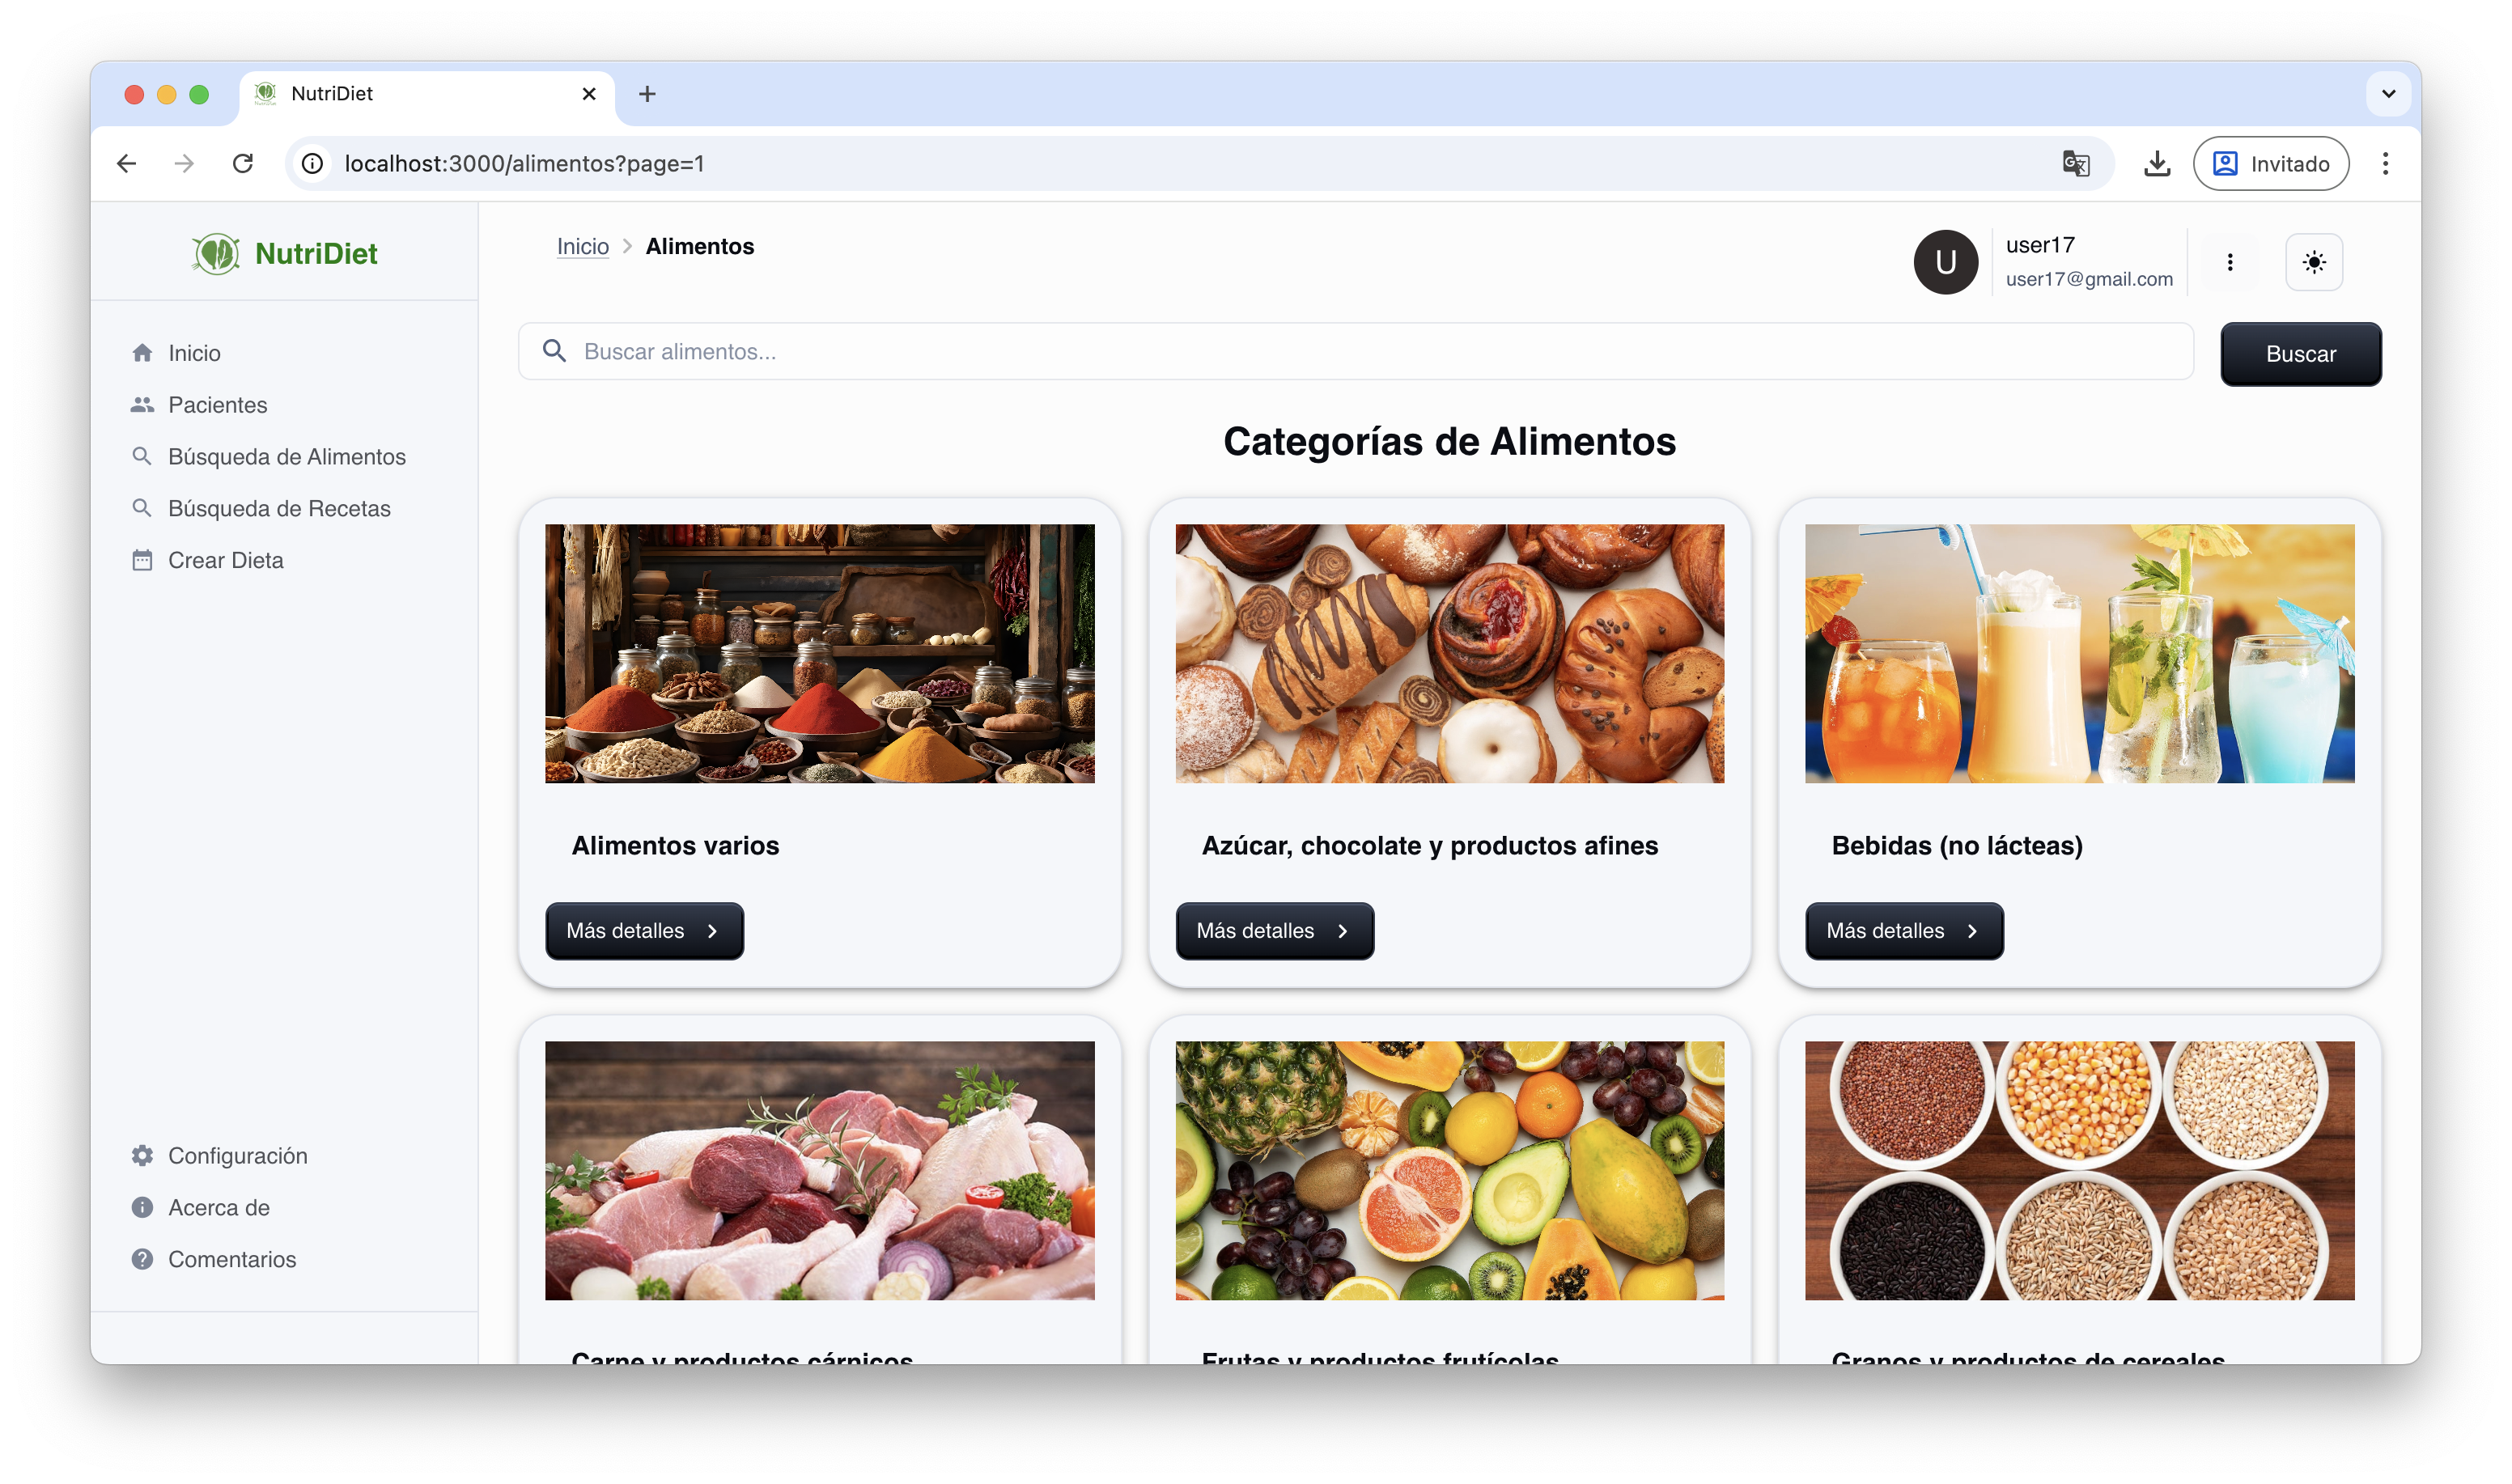
\includegraphics[width=1\linewidth]{Plantilla_TFG_latex//imagenes/Alimento_ini.png}
    \caption{Vista general del módulo de alimentos}
    \label{fig:Alimento_ini}
\end{figure}

\subsection{Búsqueda y filtrado}
El sistema proporciona una herramienta de búsqueda y filtrado avanzada para facilitar la localización de alimentos en la base de datos (Figura~\ref{fig:Alimento_Categoria}).

La barra de búsqueda permite introducir el nombre (completo o parcial) del alimento, mostrando como máximo los primeros 20 resultados coincidentes. A medida que el usuario escribe, los resultados se actualizan dinámicamente en tiempo real. 

Además de la búsqueda por texto, el sistema incluye múltiples opciones de filtrado combinables entre sí:

\begin{itemize}
    \item Por categoría: permite mostrar solo alimentos pertenecientes a un grupo específico (por ejemplo: frutas, carnes, cereales, etc.).
    
    \item Por letra inicial: útil para localizar alimentos cuando solo se conoce la primera letra del nombre (A–Z).
    
    \item Por nivel de nutrientes: el usuario puede filtrar alimentos según su contenido en sodio, azúcar o grasa, seleccionando entre tres rangos: bajo, medio o alto. Permite identificar rápidamente alimentos más saludables o adaptados a dietas específicas (como hiposódicas o bajas en azúcares).
\end{itemize}

\begin{figure}[H]
    \centering
    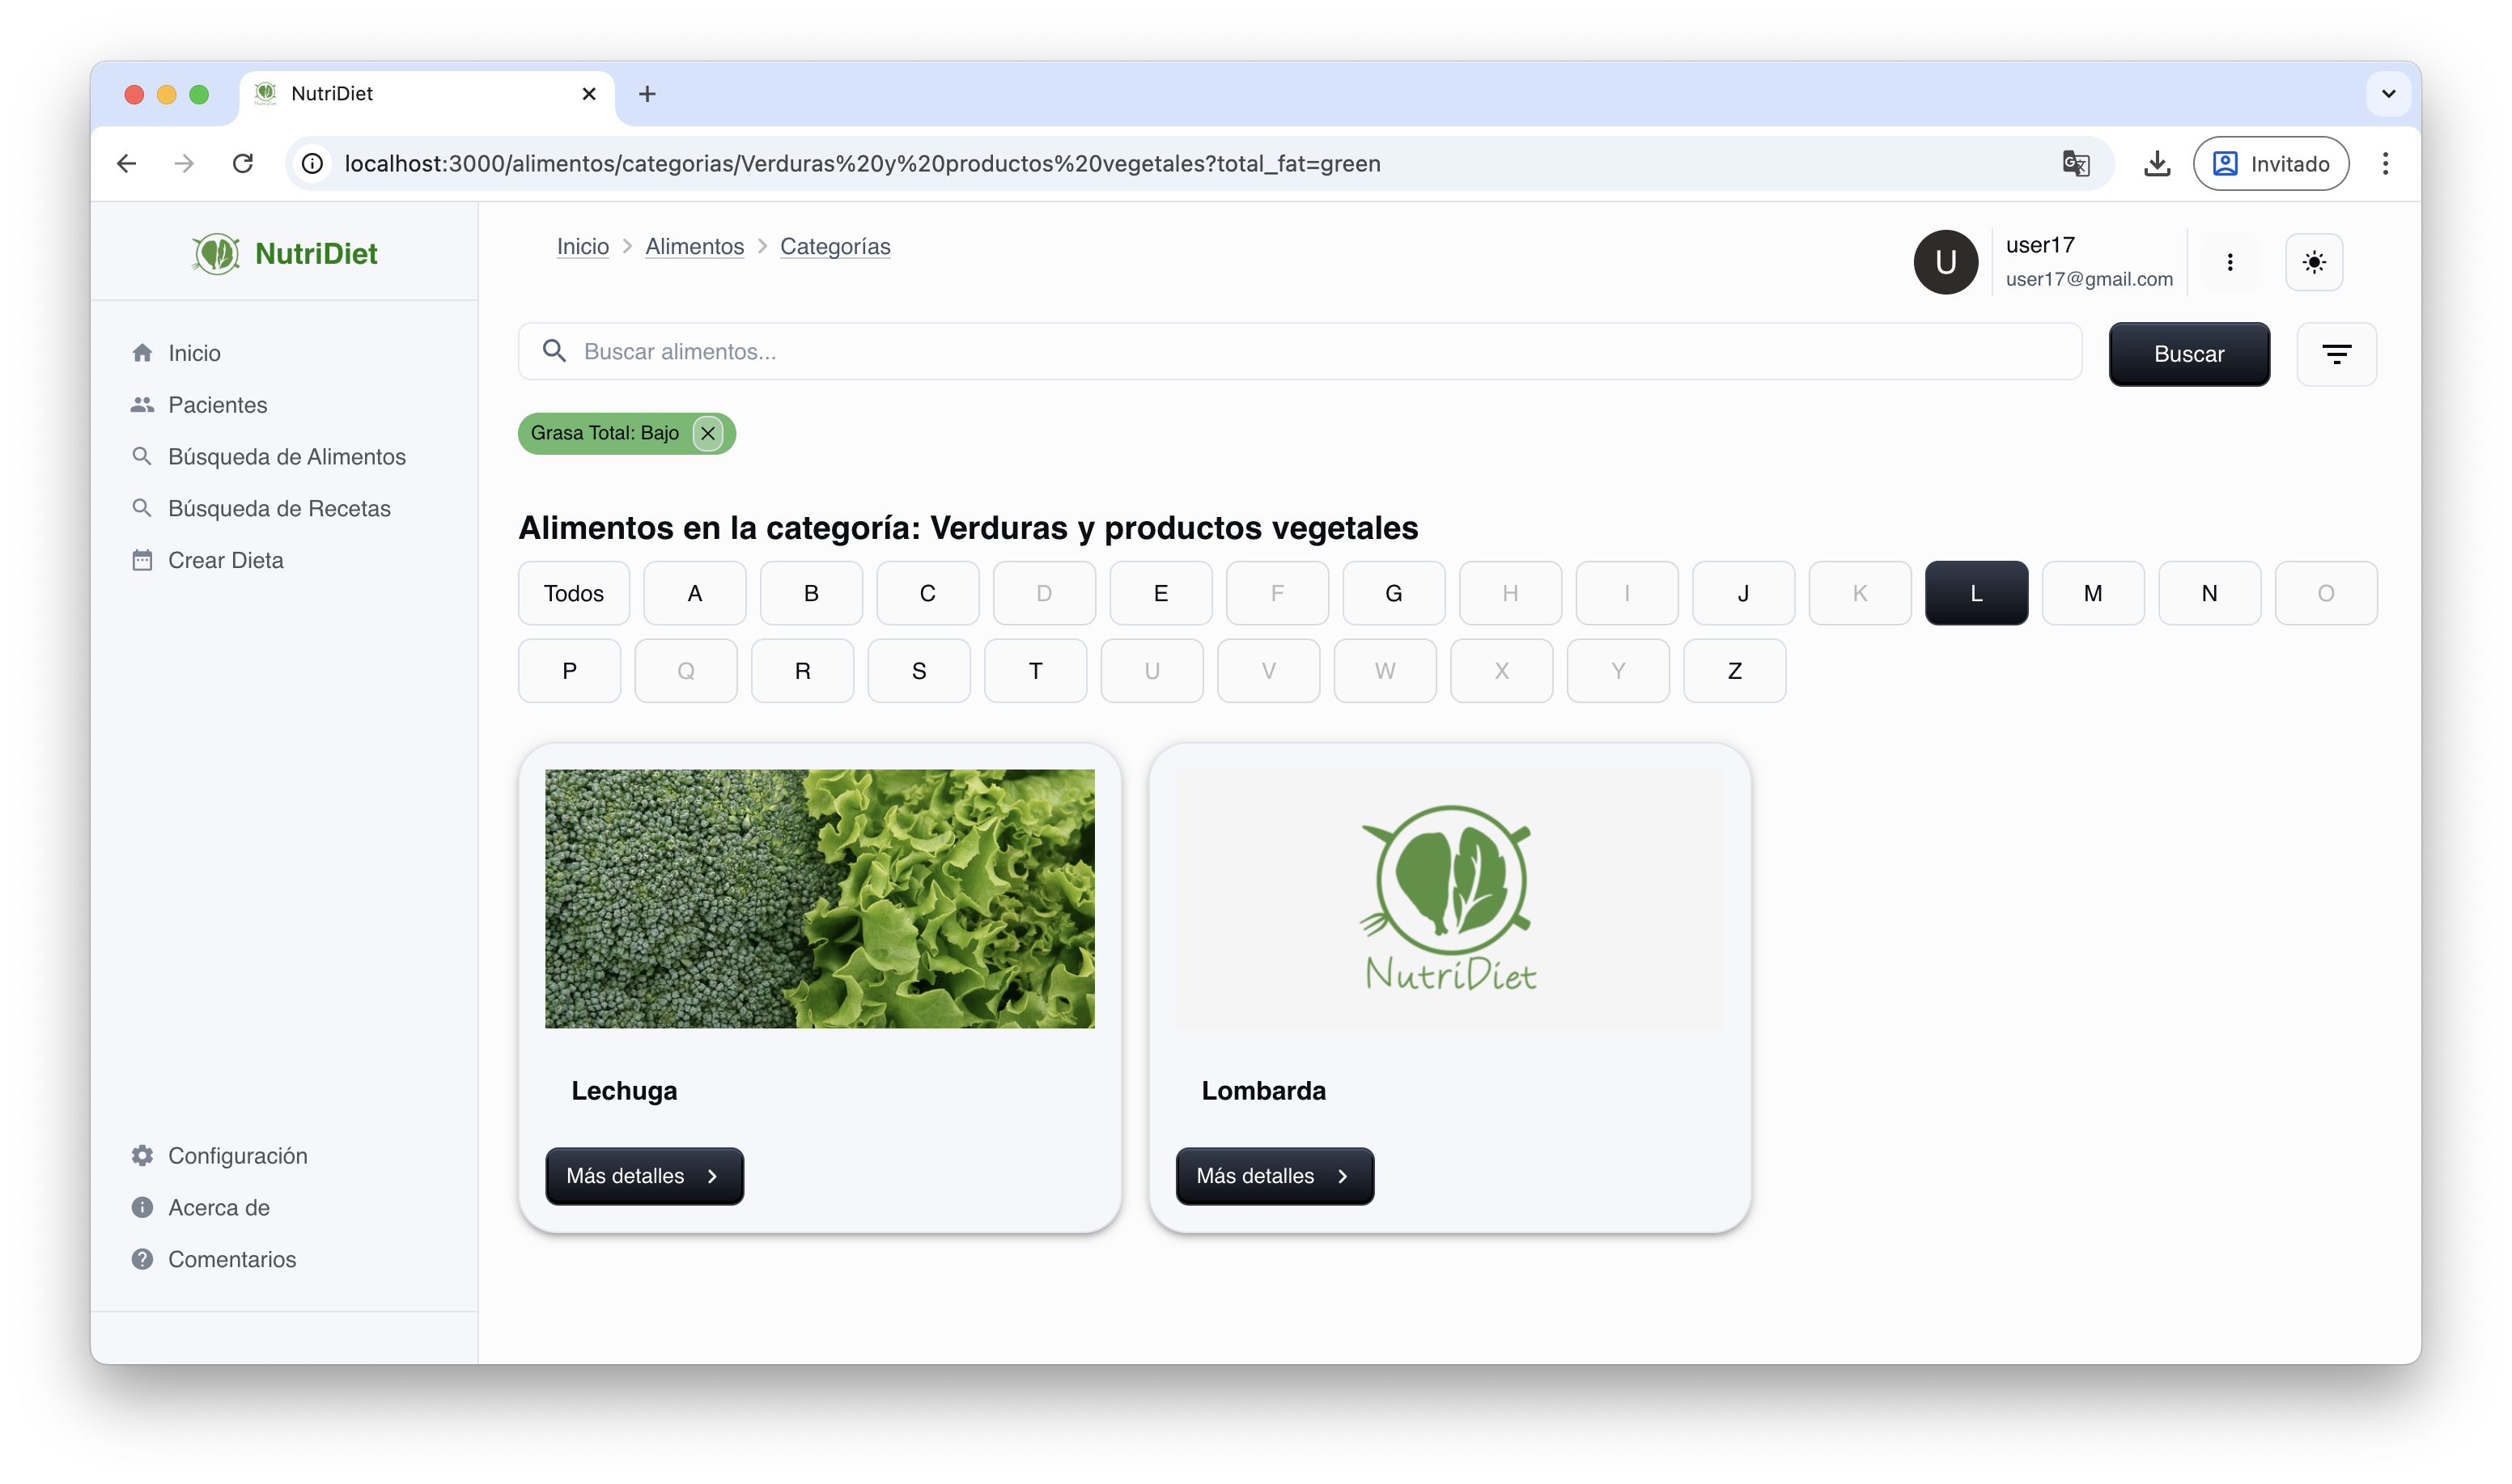
\includegraphics[width=1\linewidth]{Plantilla_TFG_latex/imagenes/Alimento_Categoria.png}
    \caption{Interfaz de búsqueda y filtrado de alimentos por nombre, categoría, letra inicial y contenido nutricional}
    \label{fig:Alimento_Categoria}
\end{figure}

\subsection{Detalle del alimento}
Esta vista muestra la información nutricional completa y organizada, acompañada de una imagen representativa, su categoría, el porcentaje comestible y el etiquetado nutricional según el sistema de semáforos de la OMS (sal, azúcar, grasa) (Figura~\ref{fig:detalle_alimento}).

En la parte principal se encuentra una tabla que presenta los valores nutricionales por 100 gramos, por porción comestible y por diferentes medidas prácticas (porciones estándar, unidades y medidas caseras como “1 cucharada” o “1 taza”), lo cual permite adaptar fácilmente el uso del alimento en recetas o dietas.

\begin{figure}[H]
    \centering
    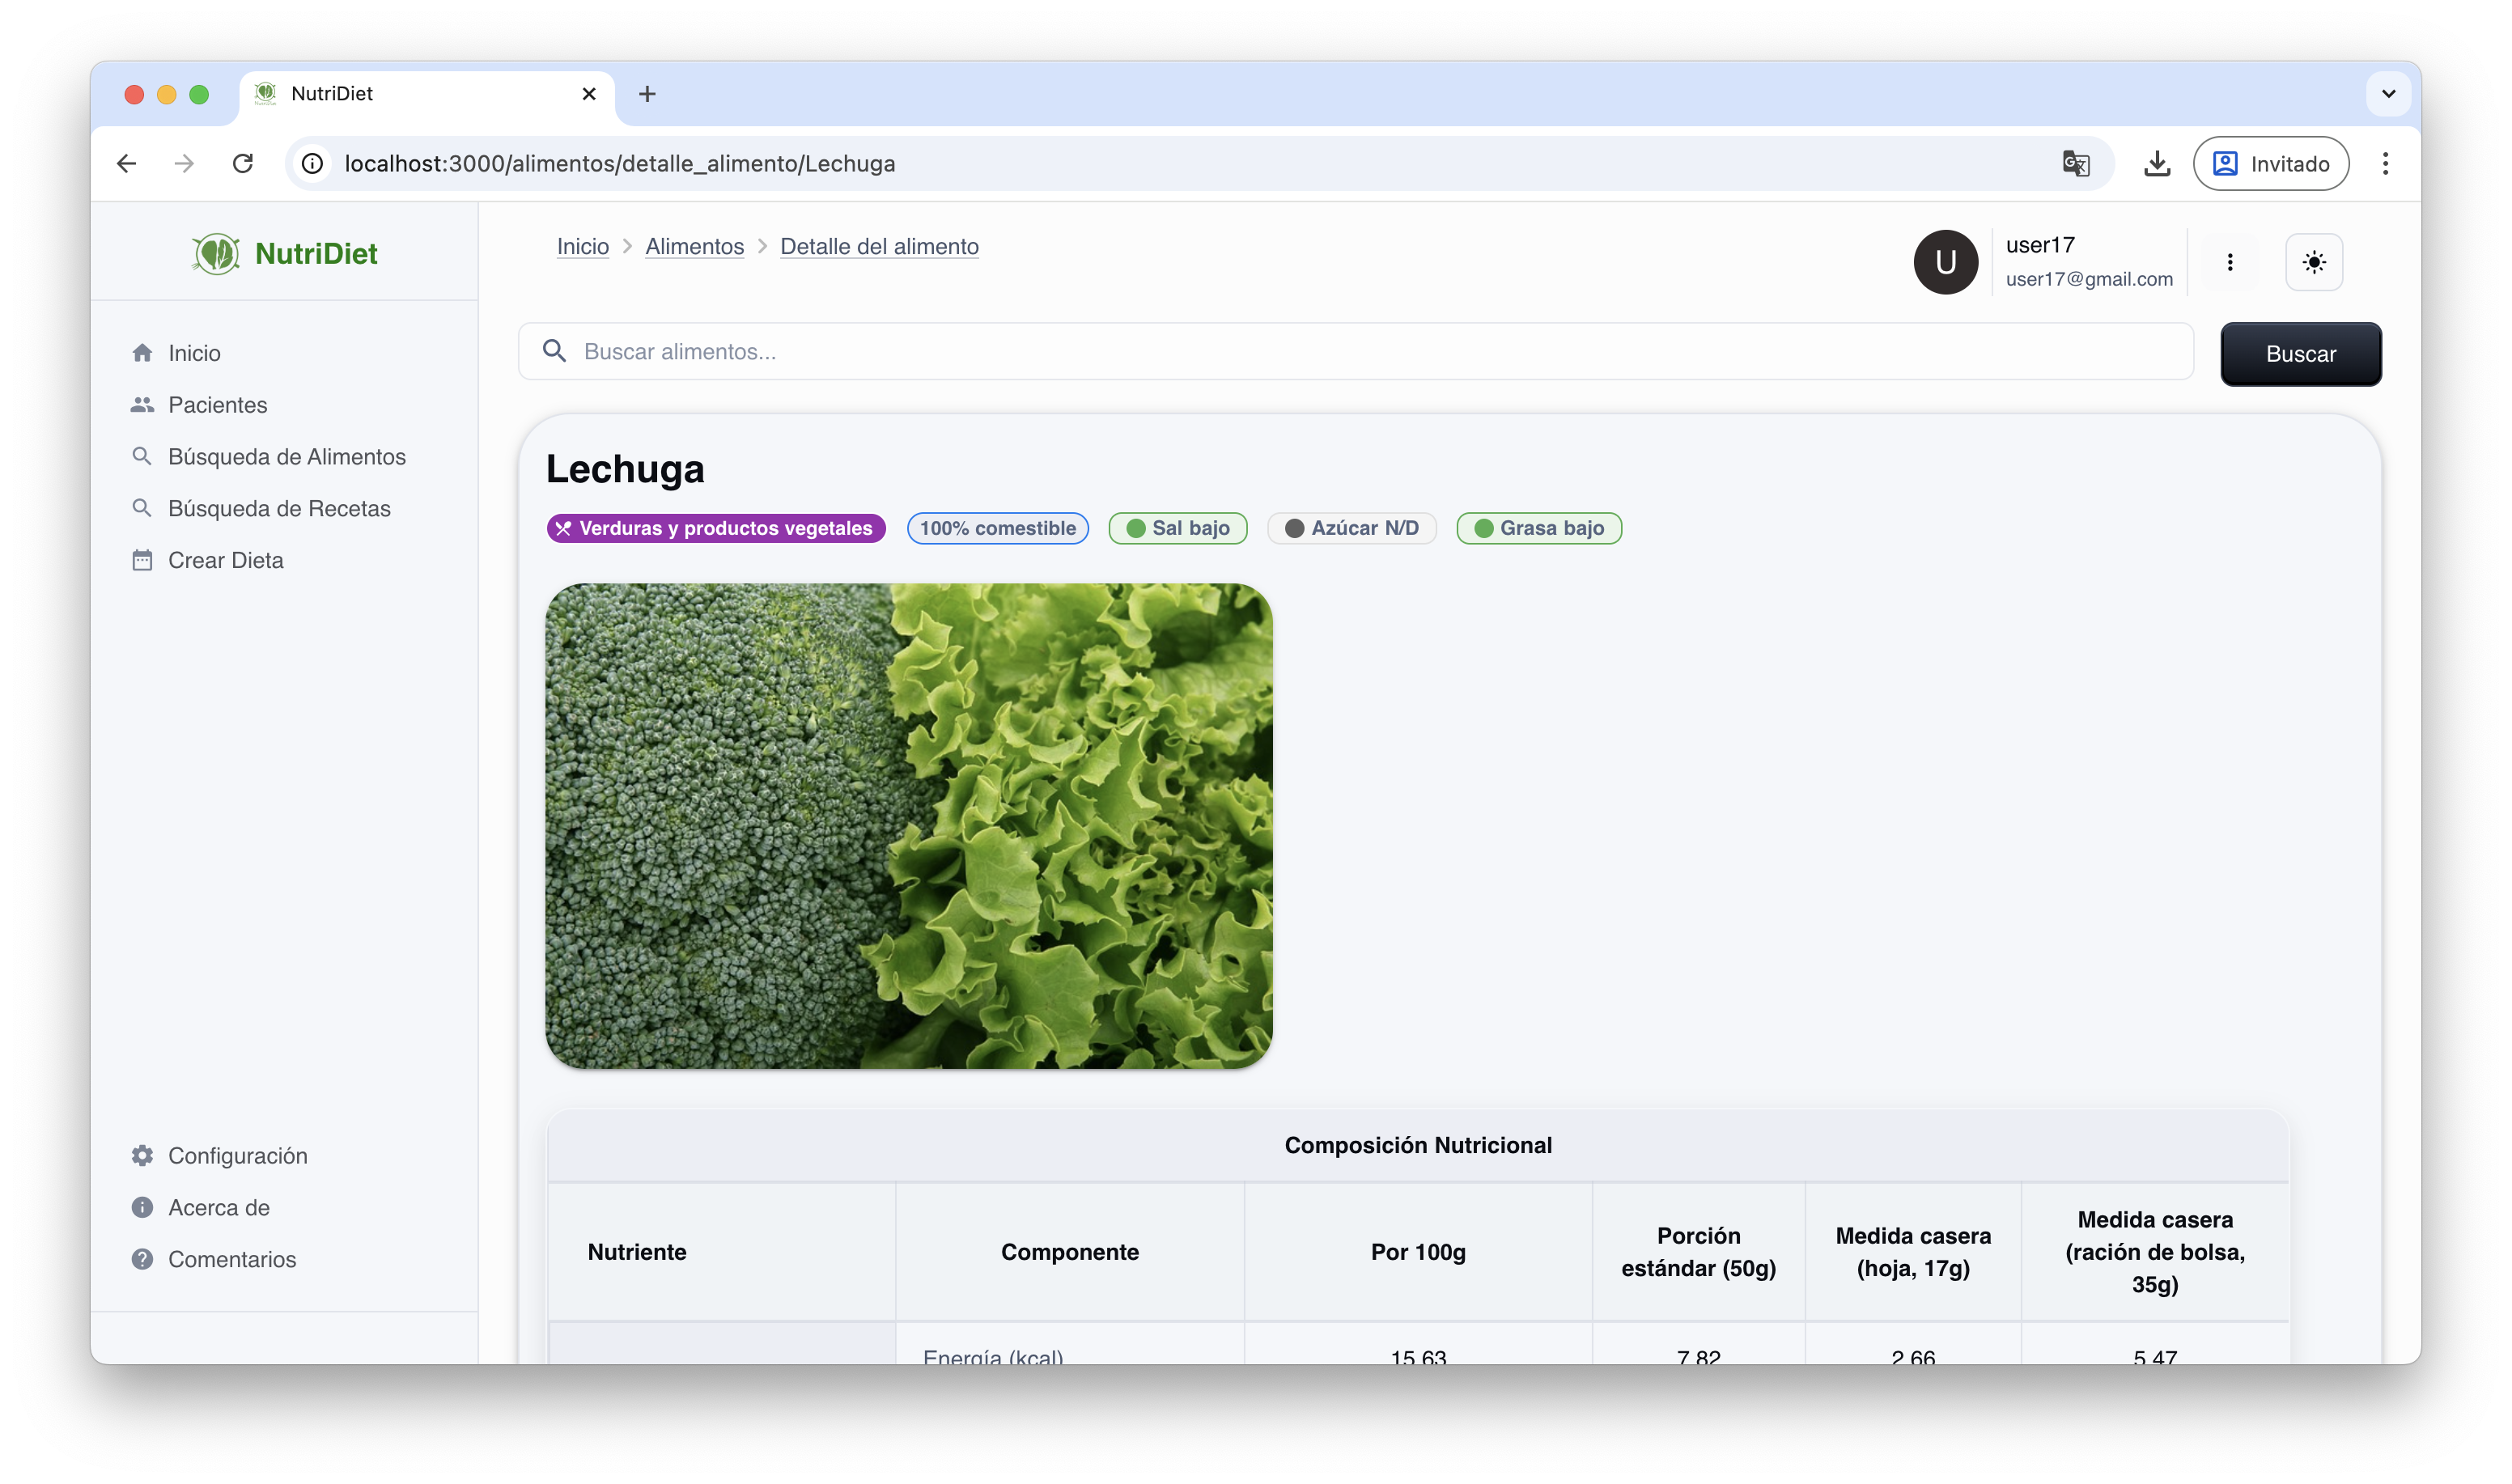
\includegraphics[width=1\linewidth]{Plantilla_TFG_latex/imagenes/PagAlimento_Detalle.png}
    \caption{Vista detallada de un alimento con tabla nutricional y porciones disponibles}
    \label{fig:detalle_alimento}
\end{figure}

\section{Consultas de recetas}
El sistema incluye un módulo específico para la búsqueda y visualización de recetas (Figura~\ref{fig:consultas_recetas}). Desde esta sección, el usuario puede explorar todas las recetas registradas, ya sea mediante navegación libre o utilizando herramientas de búsqueda y filtrado por categoría.

\begin{itemize}
    \item Listado de recetas: Muestra todas las recetas disponibles en formato de tarjetas, organizadas por categoría.

    \item Búsqueda y filtrado: Permite buscar recetas por nombre y aplicar filtros por categoría, letra inicial o por valores nutricionales (kcal, proteínas, carbohidratos).

    \item Detalle de receta: Al seleccionar una receta, se muestra su composición nutricional completa, los ingredientes, número de raciones, los pasos de preparación y un pequeño comentario nutricional.
\end{itemize}

\begin{figure}[t]
    \centering
    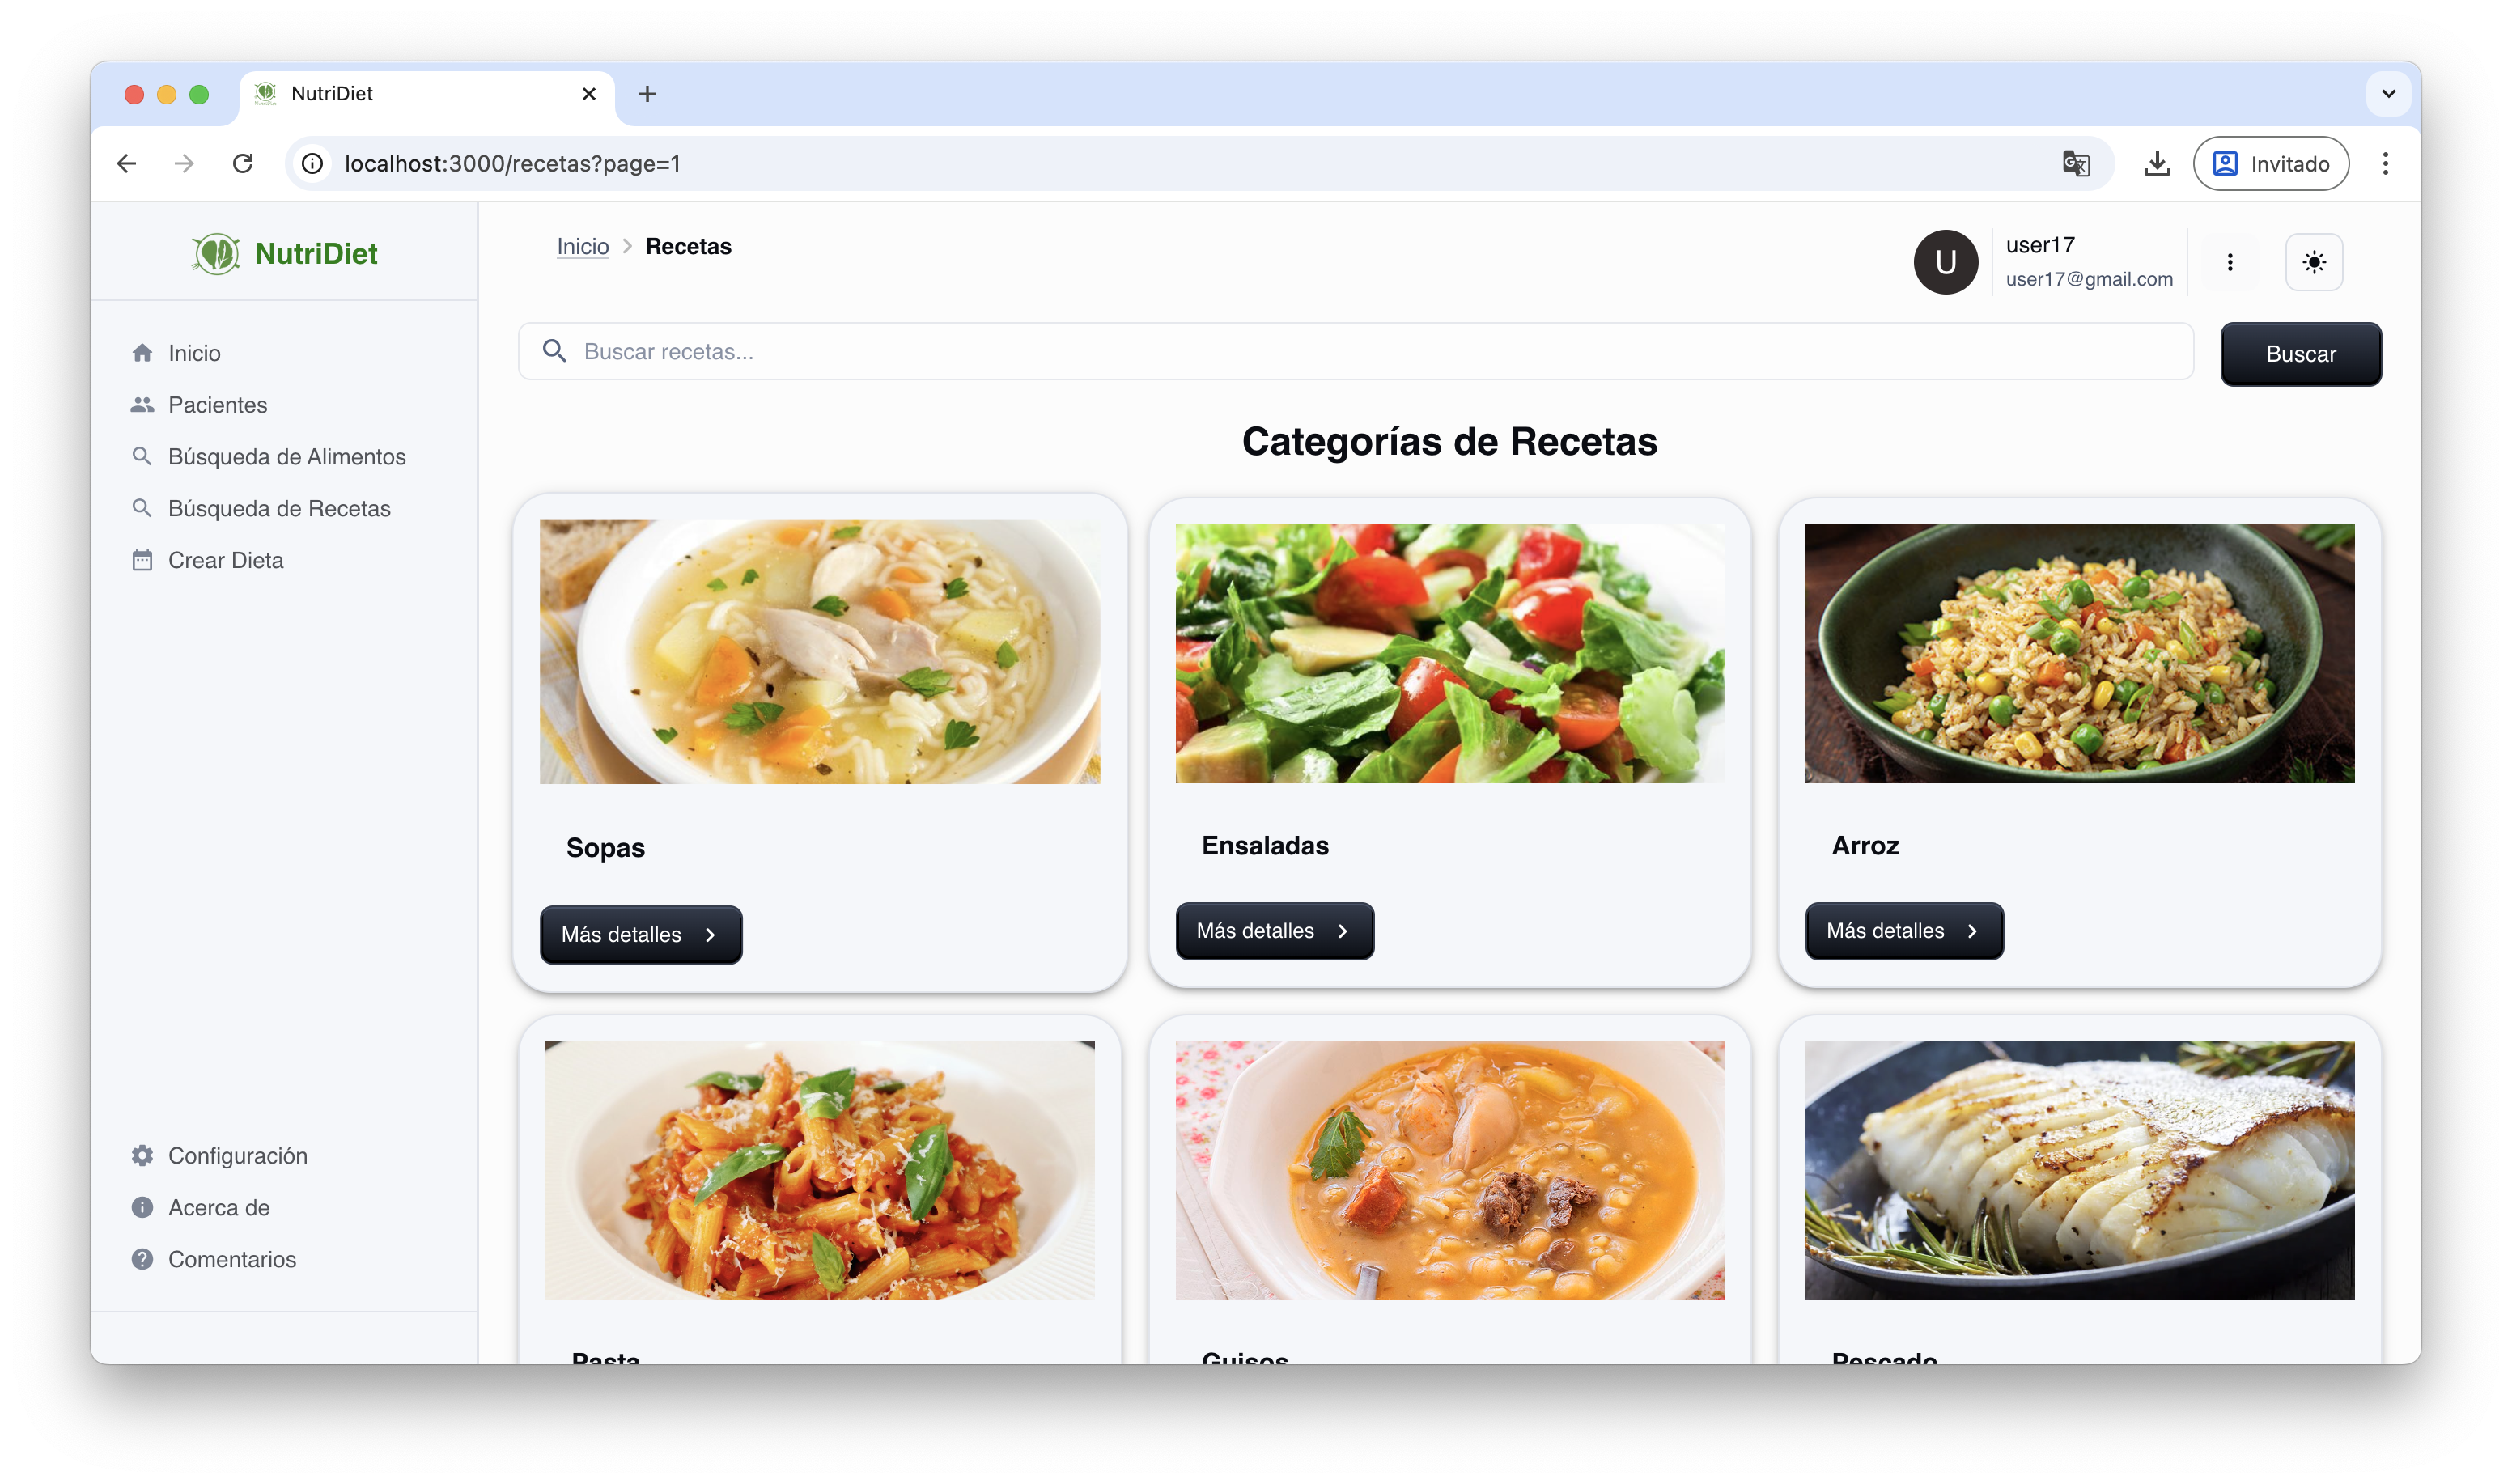
\includegraphics[width=1\linewidth]{Plantilla_TFG_latex/imagenes/Recetas_ini.png}
    \caption{Vista general del módulo de recetas con tarjetas filtrables por categoría}
    \label{fig:consultas_recetas}
\end{figure}

\subsection{Búsqueda y filtrado}
El sistema ofrece una interfaz avanzada para la búsqueda y filtrado de recetas dentro de una categoría específica. (Figura~\ref{fig:Recetas_categoria})  Esta funcionalidad permite al usuario localizar fácilmente recetas que se ajusten tanto a criterios textuales como a parámetros nutricionales específicos.

La barra de búsqueda acepta el nombre completo o parcial de una receta. A medida que se escribe, se despliega una lista de sugerencias dinámicas que permite seleccionar directamente una receta y acceder a su detalle. Este sistema de autocompletado mejora la rapidez y precisión de la búsqueda.

Además de la búsqueda textual, se incluyen varias opciones de filtrado que pueden combinarse:

\begin{itemize}
    \item Por letra inicial: muestra únicamente las recetas cuyo nombre comienza por la letra seleccionada (de la A a la Z), facilitando una exploración rápida cuando se desconoce el nombre exacto.

    \item Por contenido nutricional: el usuario puede activar filtros avanzados que permiten establecer rangos personalizados para calorías, proteínas y carbohidratos. Esta funcionalidad resulta útil para identificar recetas adaptadas a necesidades nutricionales concretas (por ejemplo, dietas hipocalóricas o altas en proteínas). Los rangos máximos se ajustan automáticamente según las recetas disponibles en la categoría.

    \item Paginación y visualización: las recetas que cumplen los criterios de búsqueda y filtrado se muestran en forma de tarjetas informativas. En caso de haber muchas coincidencias, se activa un sistema de paginación para mejorar la navegación sin recargar la vista.
\end{itemize}

\begin{figure}[H]
    \centering
    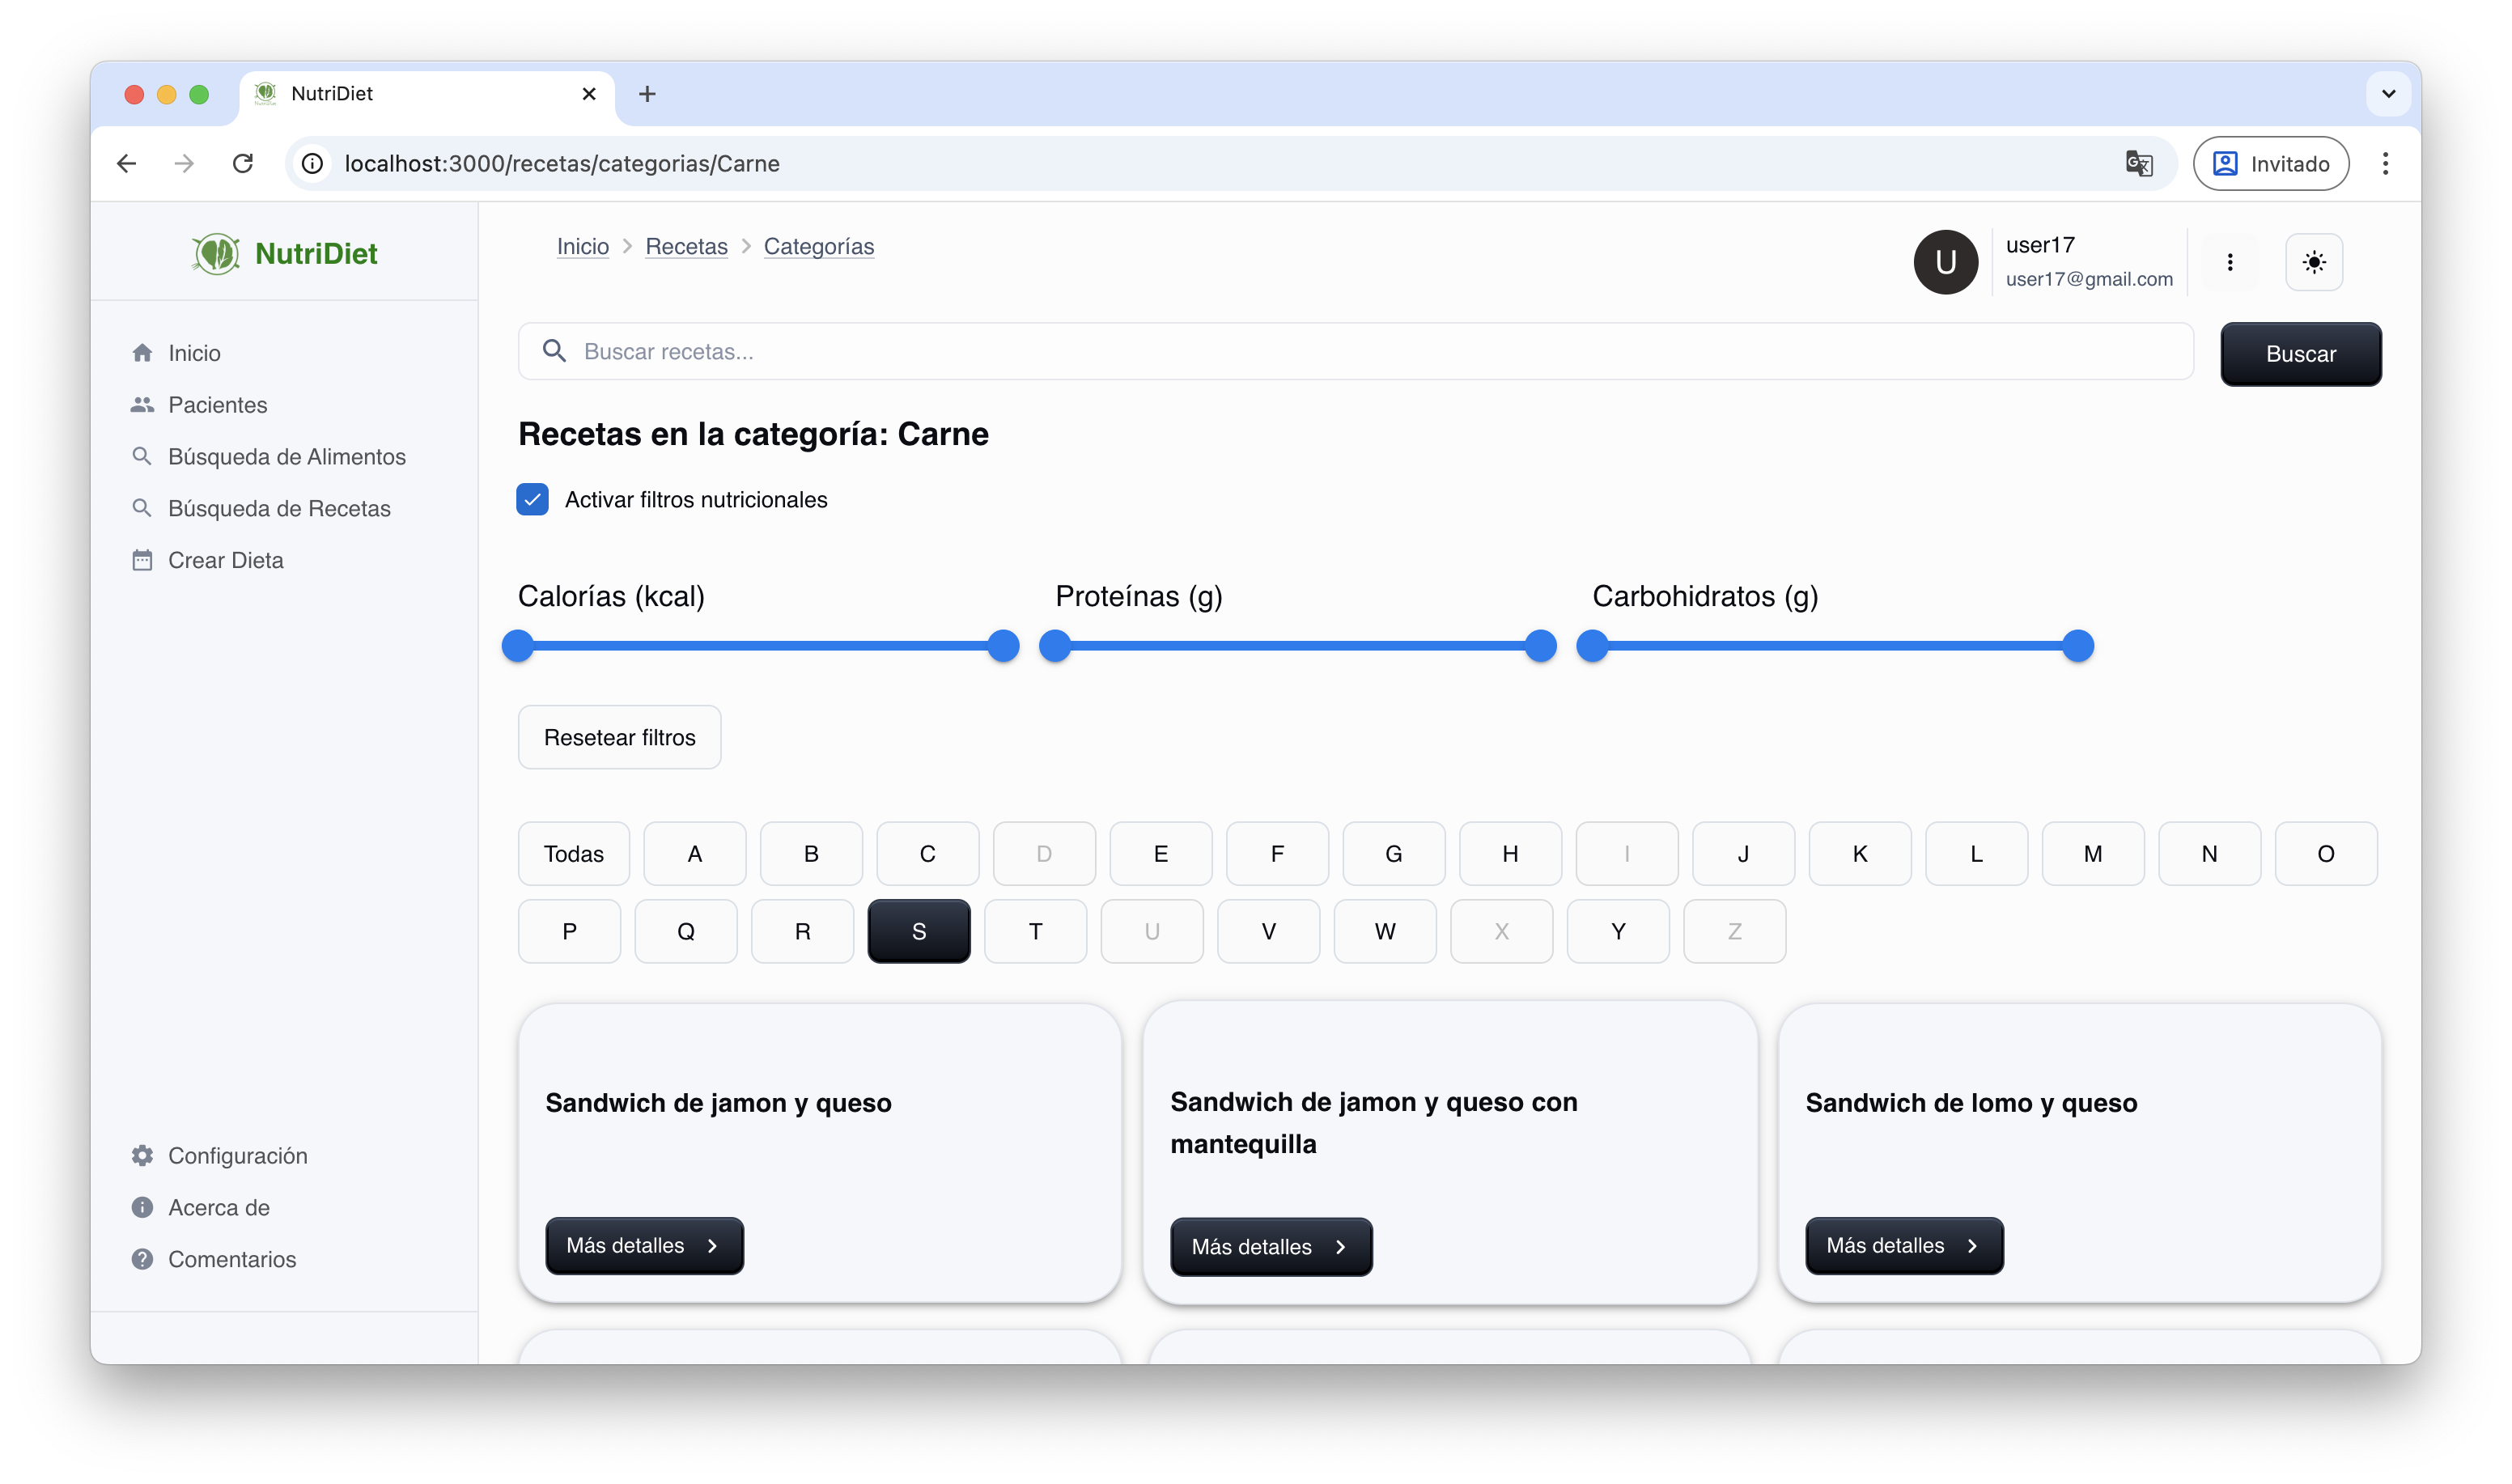
\includegraphics[width=1\linewidth]{Plantilla_TFG_latex//imagenes/Recetas_categoria.png}
    \caption{Vista de recetas filtradas por categoría con opciones de búsqueda y filtros nutricionales}
    \label{fig:Recetas_categoria}
\end{figure}


\subsection{Detalle de la receta}
La vista de detalle de una receta (Figura~\ref{fig:detalle-receta}) proporciona una descripción completa del plato, con información tanto culinaria como nutricional. En la parte superior se presenta el nombre de la receta acompañado de su categoría, país de origen, número de raciones y tiempo estimado de preparación. También se muestran etiquetas que identifican sus características dietéticas (por ejemplo: “Sin gluten”, “Bajo en grasa”) y su nivel de dificultad.

A continuación, se despliega el listado de ingredientes necesarios y los pasos detallados para su preparación. Ambos elementos están organizados en secciones colapsables que permiten una lectura cómoda y ordenada.

También tiene una tabla nutricional como los alimentos, que presenta los valores de energía, macronutrientes y micronutrientes por ración. Estos datos son calculados automáticamente a partir de los ingredientes vinculados a la receta y permiten evaluar el aporte nutricional del plato en relación con las necesidades diarias.

Además, se incluye un apartado con el comentario nutricional del profesional con fuente de origen, el cual ofrece observaciones relevantes sobre el perfil nutricional de la receta, posibles beneficios para la salud o recomendaciones para adaptar su consumo en diferentes tipos de dieta.

Finalmente, si existen otras recetas similares o relacionadas, se muestran como sugerencias para facilitar la navegación y fomentar la exploración de opciones alternativas dentro del sistema.

\begin{figure}[H]
    \centering
    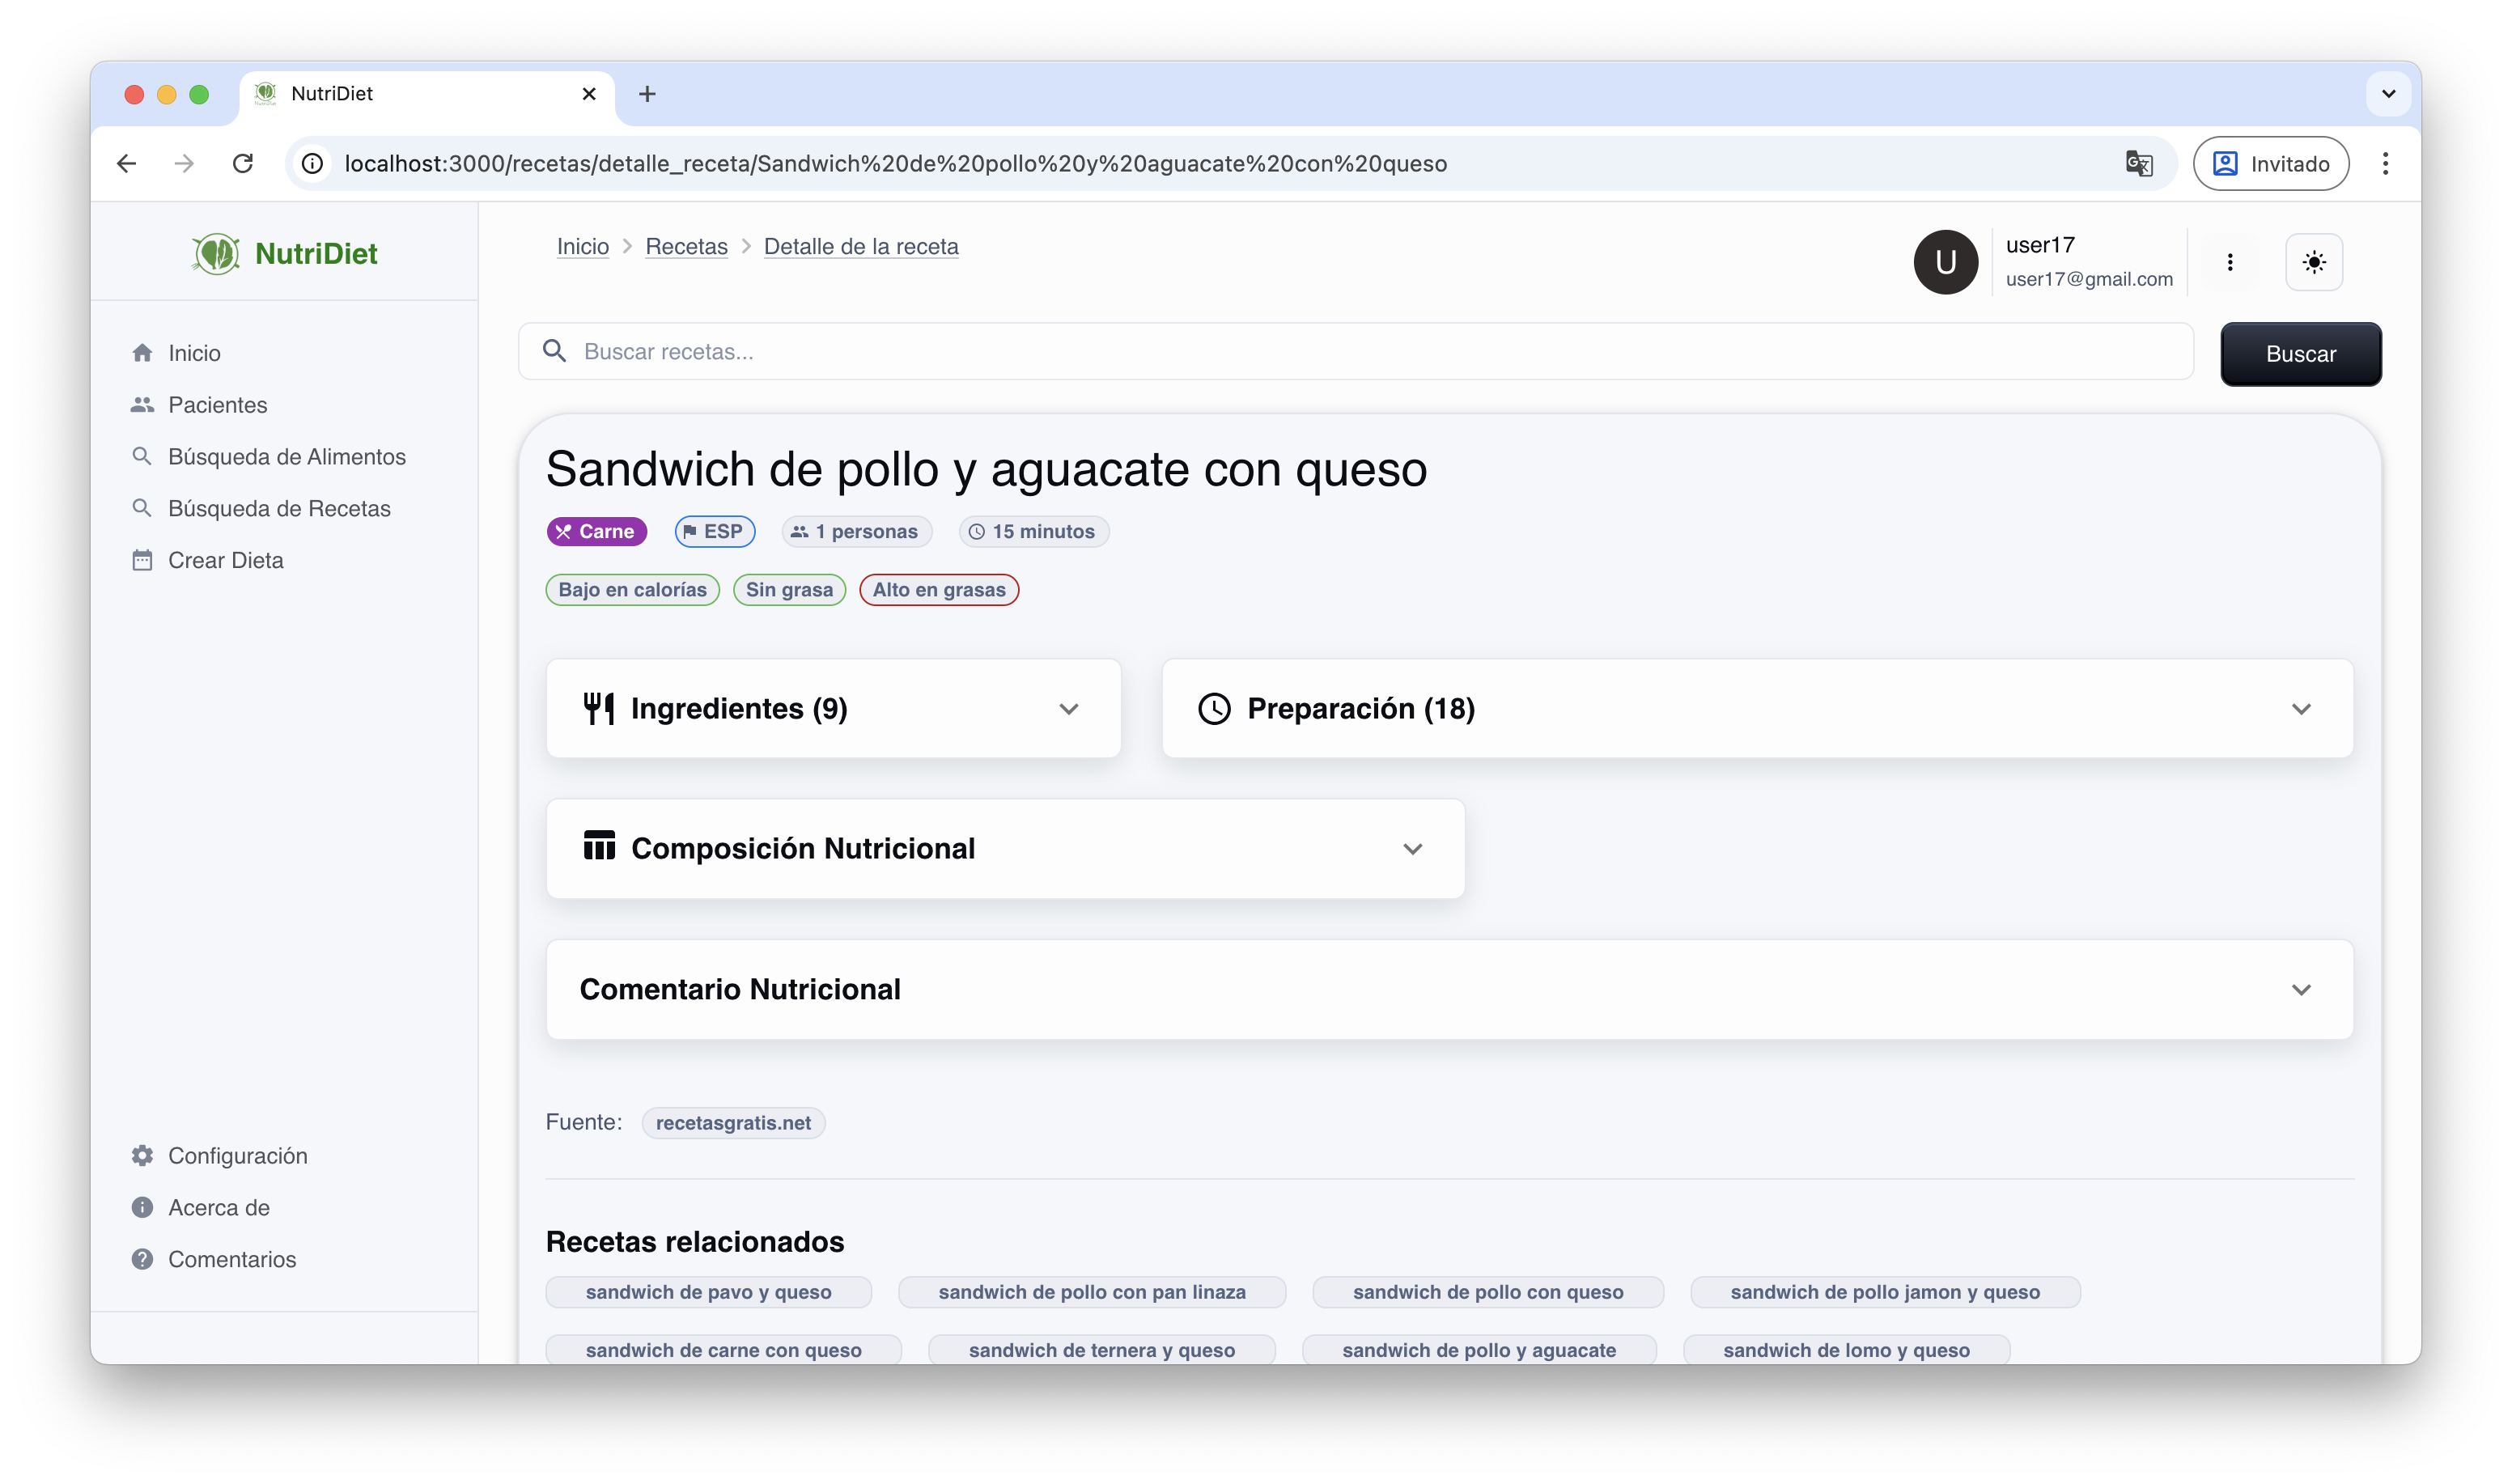
\includegraphics[width=1\linewidth]{Plantilla_TFG_latex//imagenes/Receta_detalle.png}
    \caption{Vista detallada de una receta con información nutricional, ingredientes, pasos de preparación y sugerencias relacionadas.}
    \label{fig:detalle-receta}
\end{figure}

\section{Planificación de dietas}
La funcionalidad de planificación de dietas (Figura~\ref{fig:PD_seleccionP}) permite al nutricionista diseñar, visualizar y gestionar menús estructurados para cada paciente a lo largo del tiempo. Una dieta está compuesta por un conjunto de días, y cada día incluye varias ingestas (por ejemplo: desayuno, almuerzo, cena), las cuales a su vez están formadas por recetas seleccionadas y clasificadas según el tipo de plato: entrante, primer plato, segundo plato, postre o bebida.

El proceso de planificación comienza seleccionando un paciente desde el panel correspondiente. Mientras no se haya seleccionado ningún paciente, el botón ``Continuar'' permanece deshabilitado (en gris) para evitar acciones prematuras. Este botón se habilita automáticamente y se muestra de forma destacada una vez que se ha elegido un paciente válido, guiando al nutricionista hacia el siguiente paso de la planificación. 

\begin{figure}[t]
    \centering
    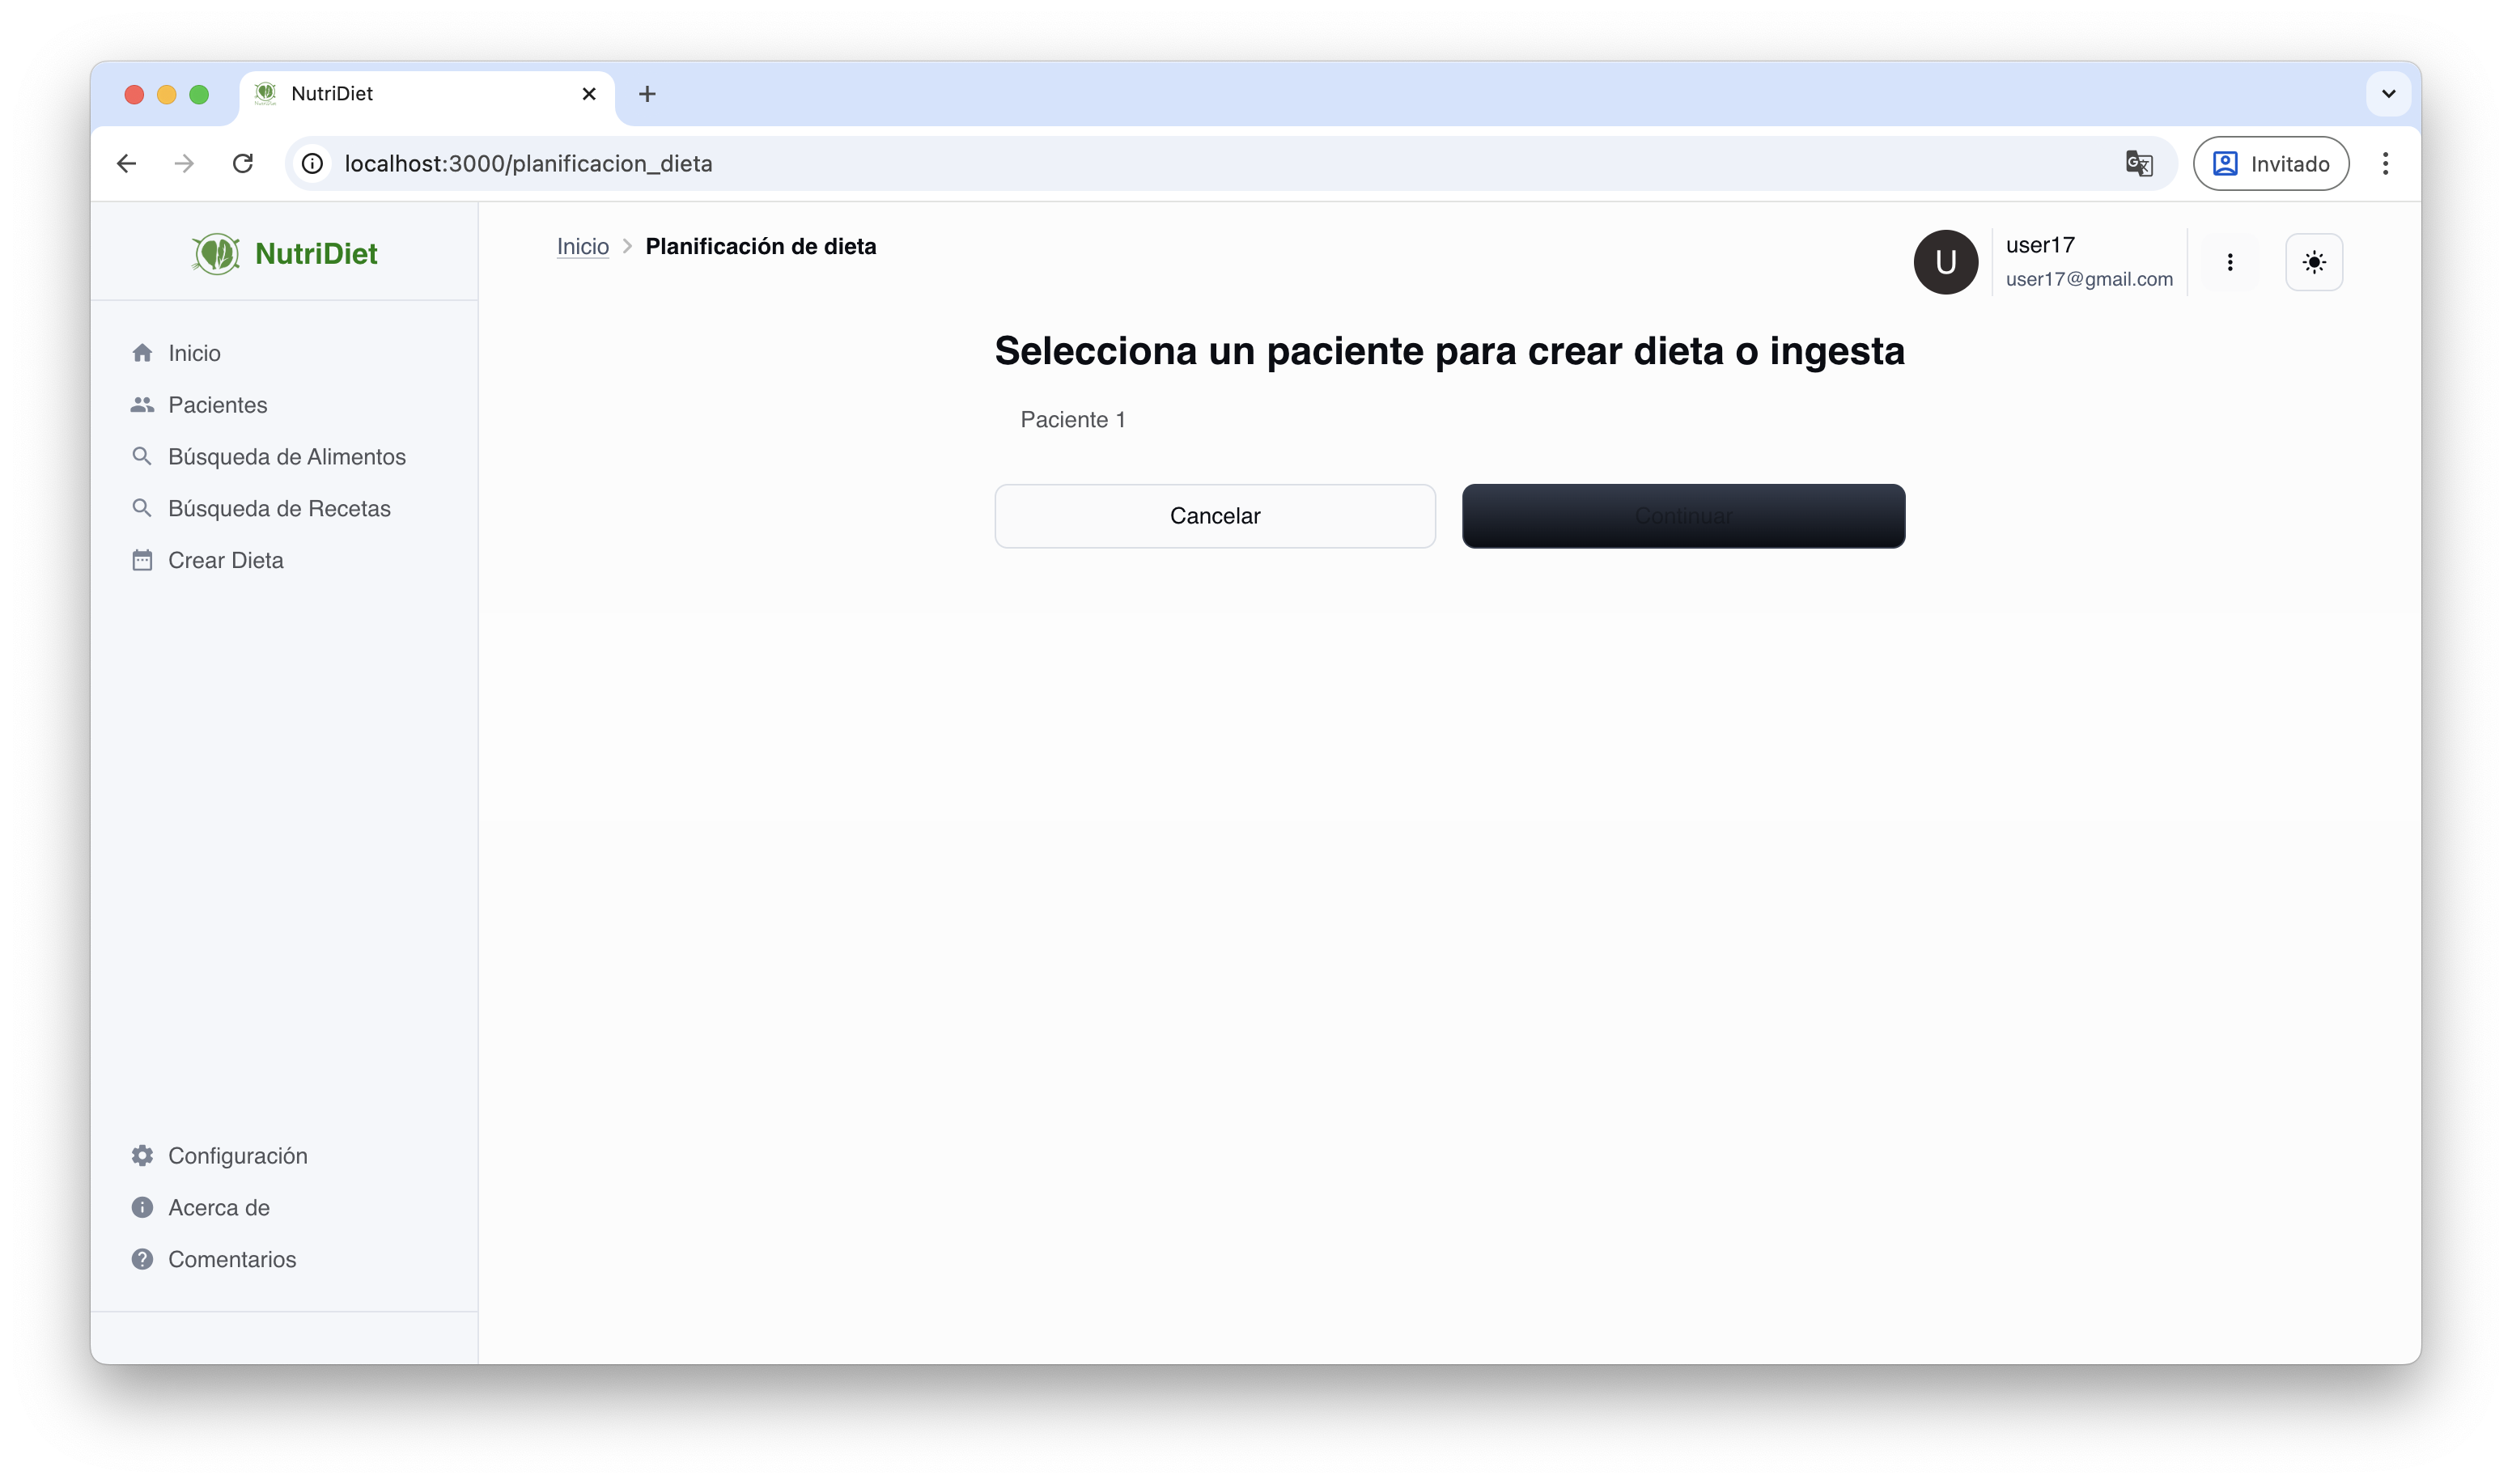
\includegraphics[width=1\linewidth]{Plantilla_TFG_latex//imagenes/PD_seleccionP.png}
    \caption{Vista de selección de paciente}
    \label{fig:PD_seleccionP}
\end{figure}

A partir de ahí, el sistema ofrece dos pestañas diferenciadas (Figura~\ref{fig:PD_ini}): una para gestionar dietas y otra para controlar las ingestas. Ambas vistas permiten crear, editar o eliminar elementos de manera independiente, manteniendo así un control granular sobre la planificación nutricional del paciente.

En la pestaña de ``Dietas'', el usuario puede:
\begin{itemize}
    \item Visualizar todas las dietas registradas del paciente, ordenadas por fecha.
    \item Aplicar filtros por año o por mes para localizar fácilmente las dietas de un periodo concreto.
    \item Identificar rápidamente la dieta activa, resaltada en un color distintivo respecto al resto.
    \item Acceder a los detalles de cada dieta mediante una tarjeta expandible, que muestra las fechas de inicio y fin, el número de días planificados y un resumen de ingestas por día.
    \item Funciones para crear una nueva dieta personalizada, editar/eliminar una dieta previa.
\end{itemize}

En la pestaña de ``Ingestas'', se ofrece un listado de todas las ingestas individuales asignadas al paciente. Esta sección incluye:
\begin{itemize}
    \item Filtros por tipo de ingesta (desayuno, media mañana, almuerzo, merienda, cena) para facilitar la navegación.
    \item Tarjetas con diseño plegable que revelan información específica al expandirse: nombre de la ingesta, recetas incluidas clasificadas por tipo de plato, comentarios nutricionales y número de raciones.
    \item Funciones para crear una nueva ingesta personalizada, reutilizar una ingesta existente o editar/eliminar una previa.
\end{itemize}

\begin{figure}[H]
    \centering
    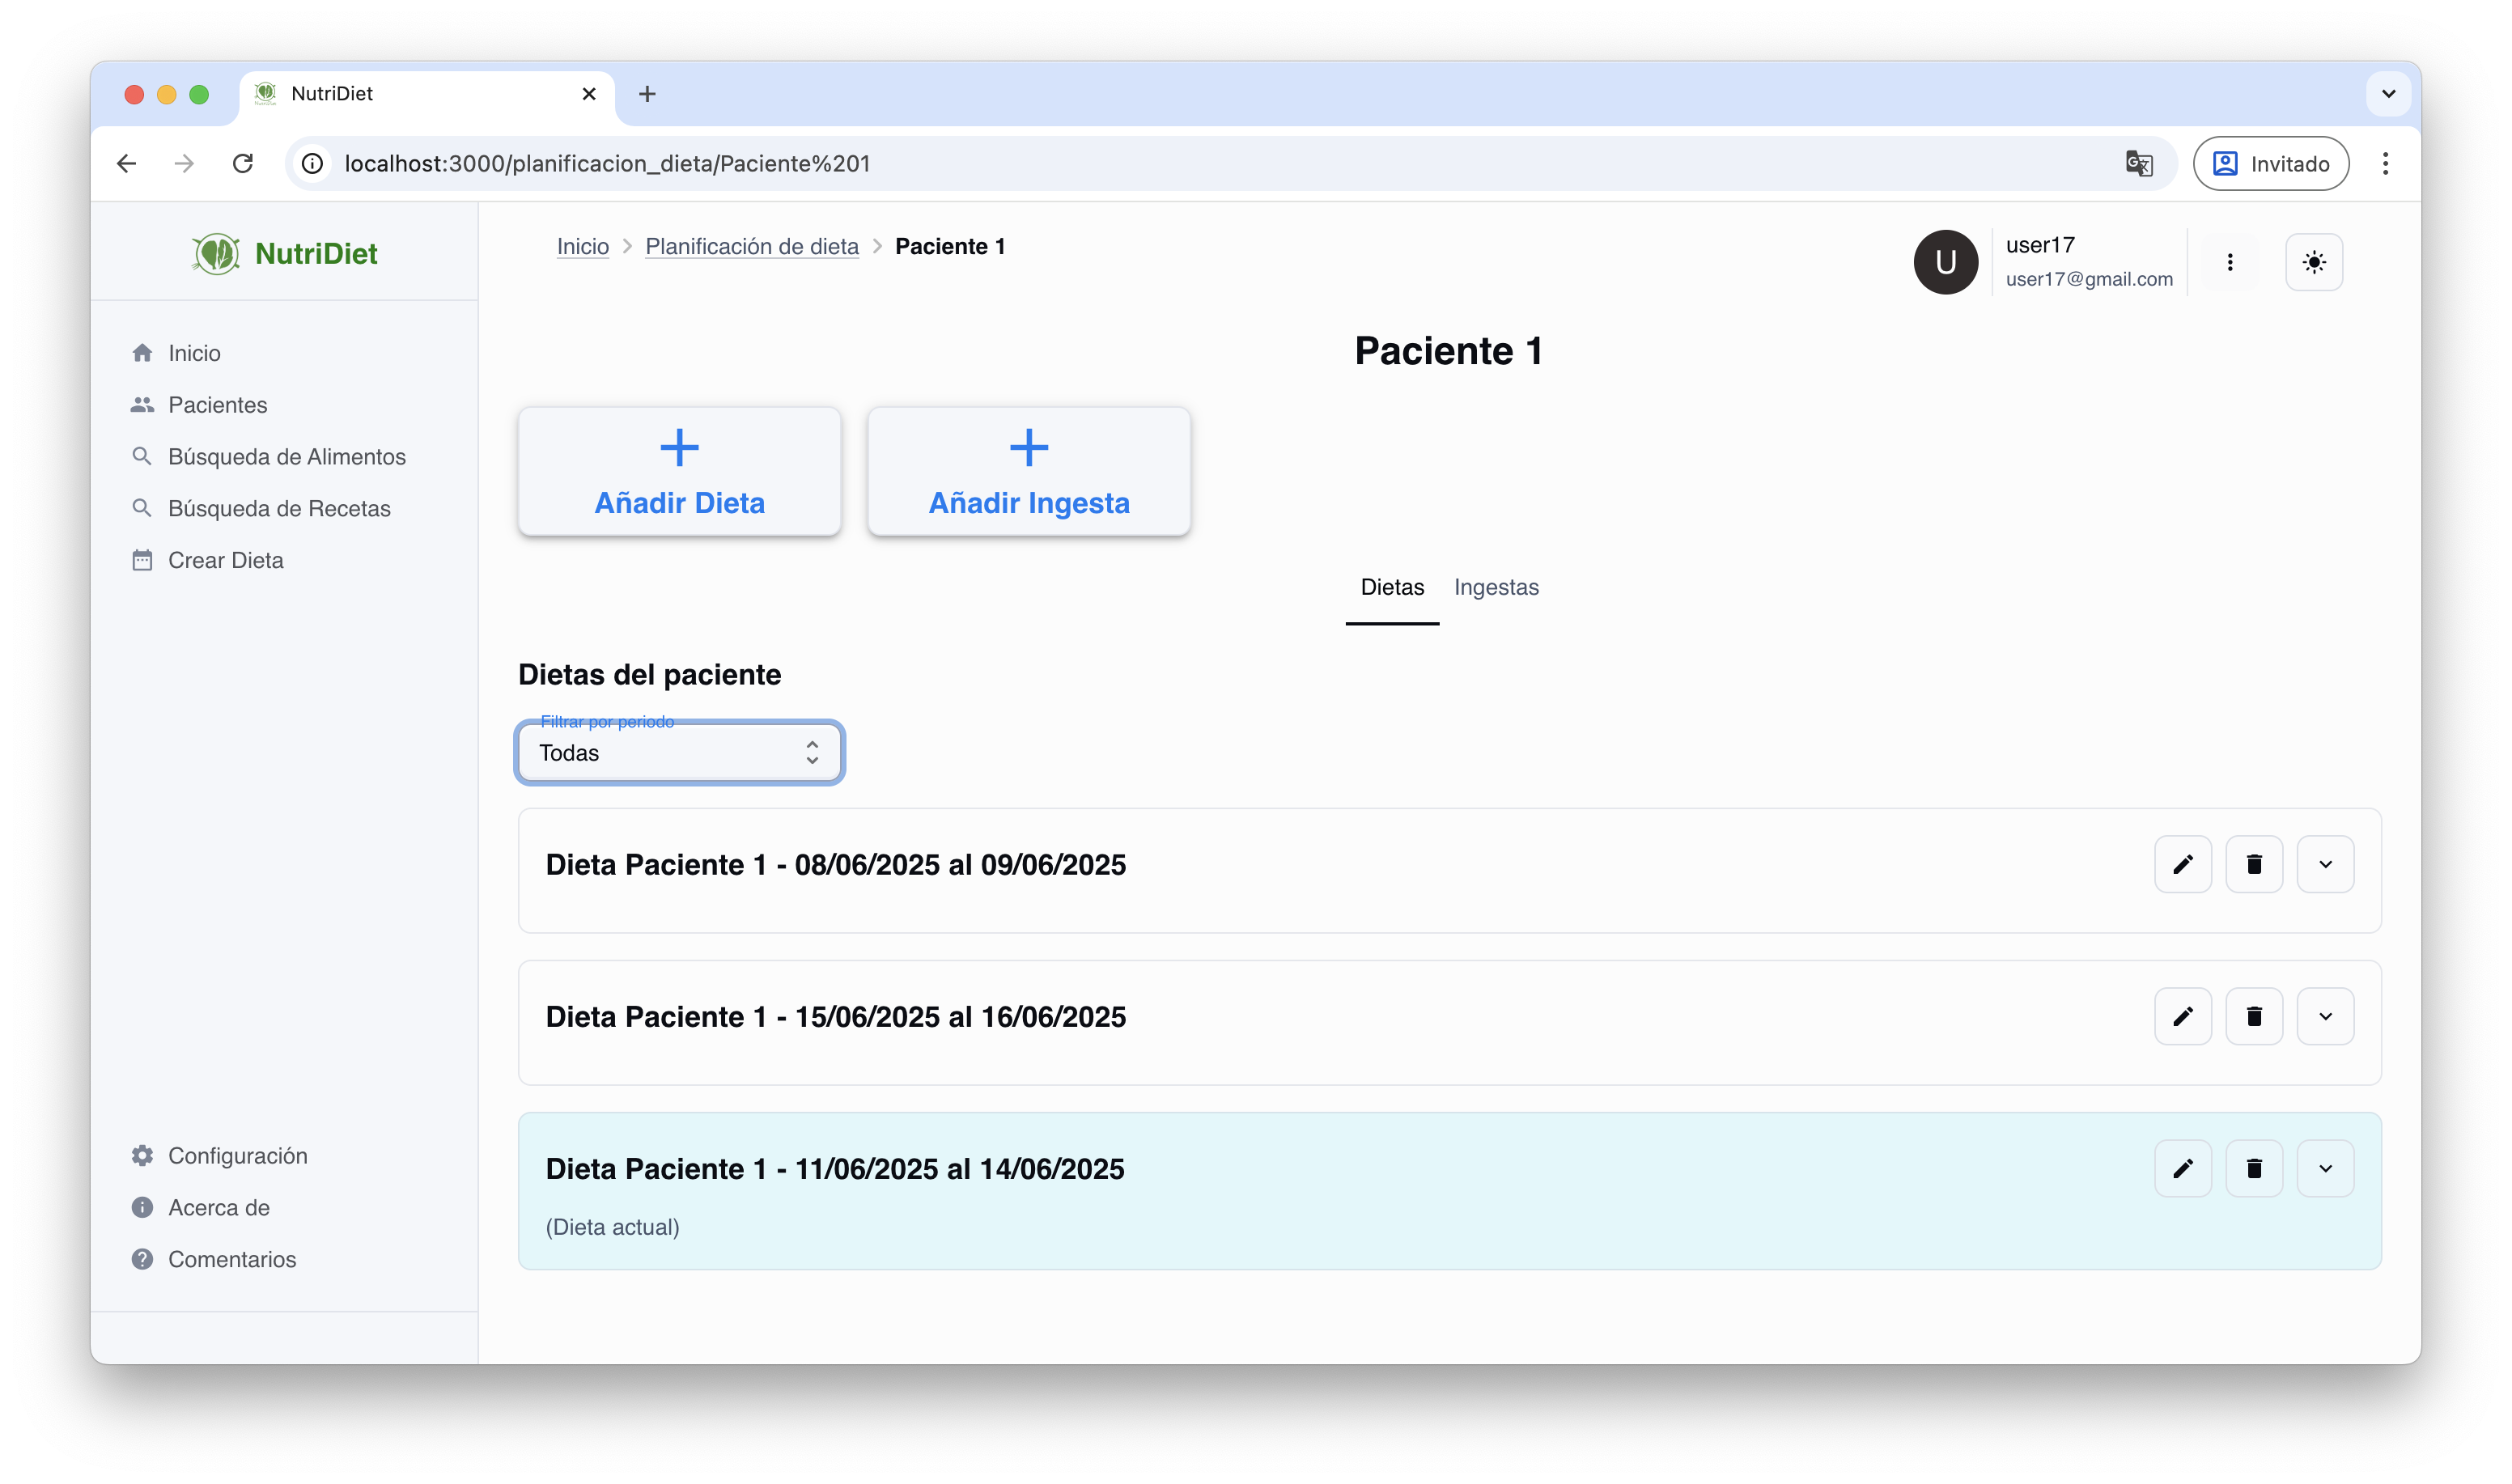
\includegraphics[width=1\linewidth]{Plantilla_TFG_latex//imagenes/PD_ini.png}
    \caption{Vista de planificación de dietas con pestañas para dietas e ingestas}
    \label{fig:PD_ini}
\end{figure}

\subsection{Crear ingesta}
El sistema permite crear una ingesta personalizada para un paciente concreto o ingestas universales que pueden ser utilizadas por todos los pacientes, especificando el nombre de la ingesta, el tipo de comida (por ejemplo: desayuno, almuerzo, cena) y las recetas que la componen, clasificadas según su función dentro del menú (entrante, primer plato, segundo plato, postre o bebida).

El proceso de creación comienza con un formulario (Figura~\ref{fig:crear-ingesta-form}) donde se debe introducir el nombre de la ingesta y seleccionar el tipo correspondiente. Esta información inicial es obligatoria para continuar con el diseño del contenido.

\begin{figure}[t]
    \centering
    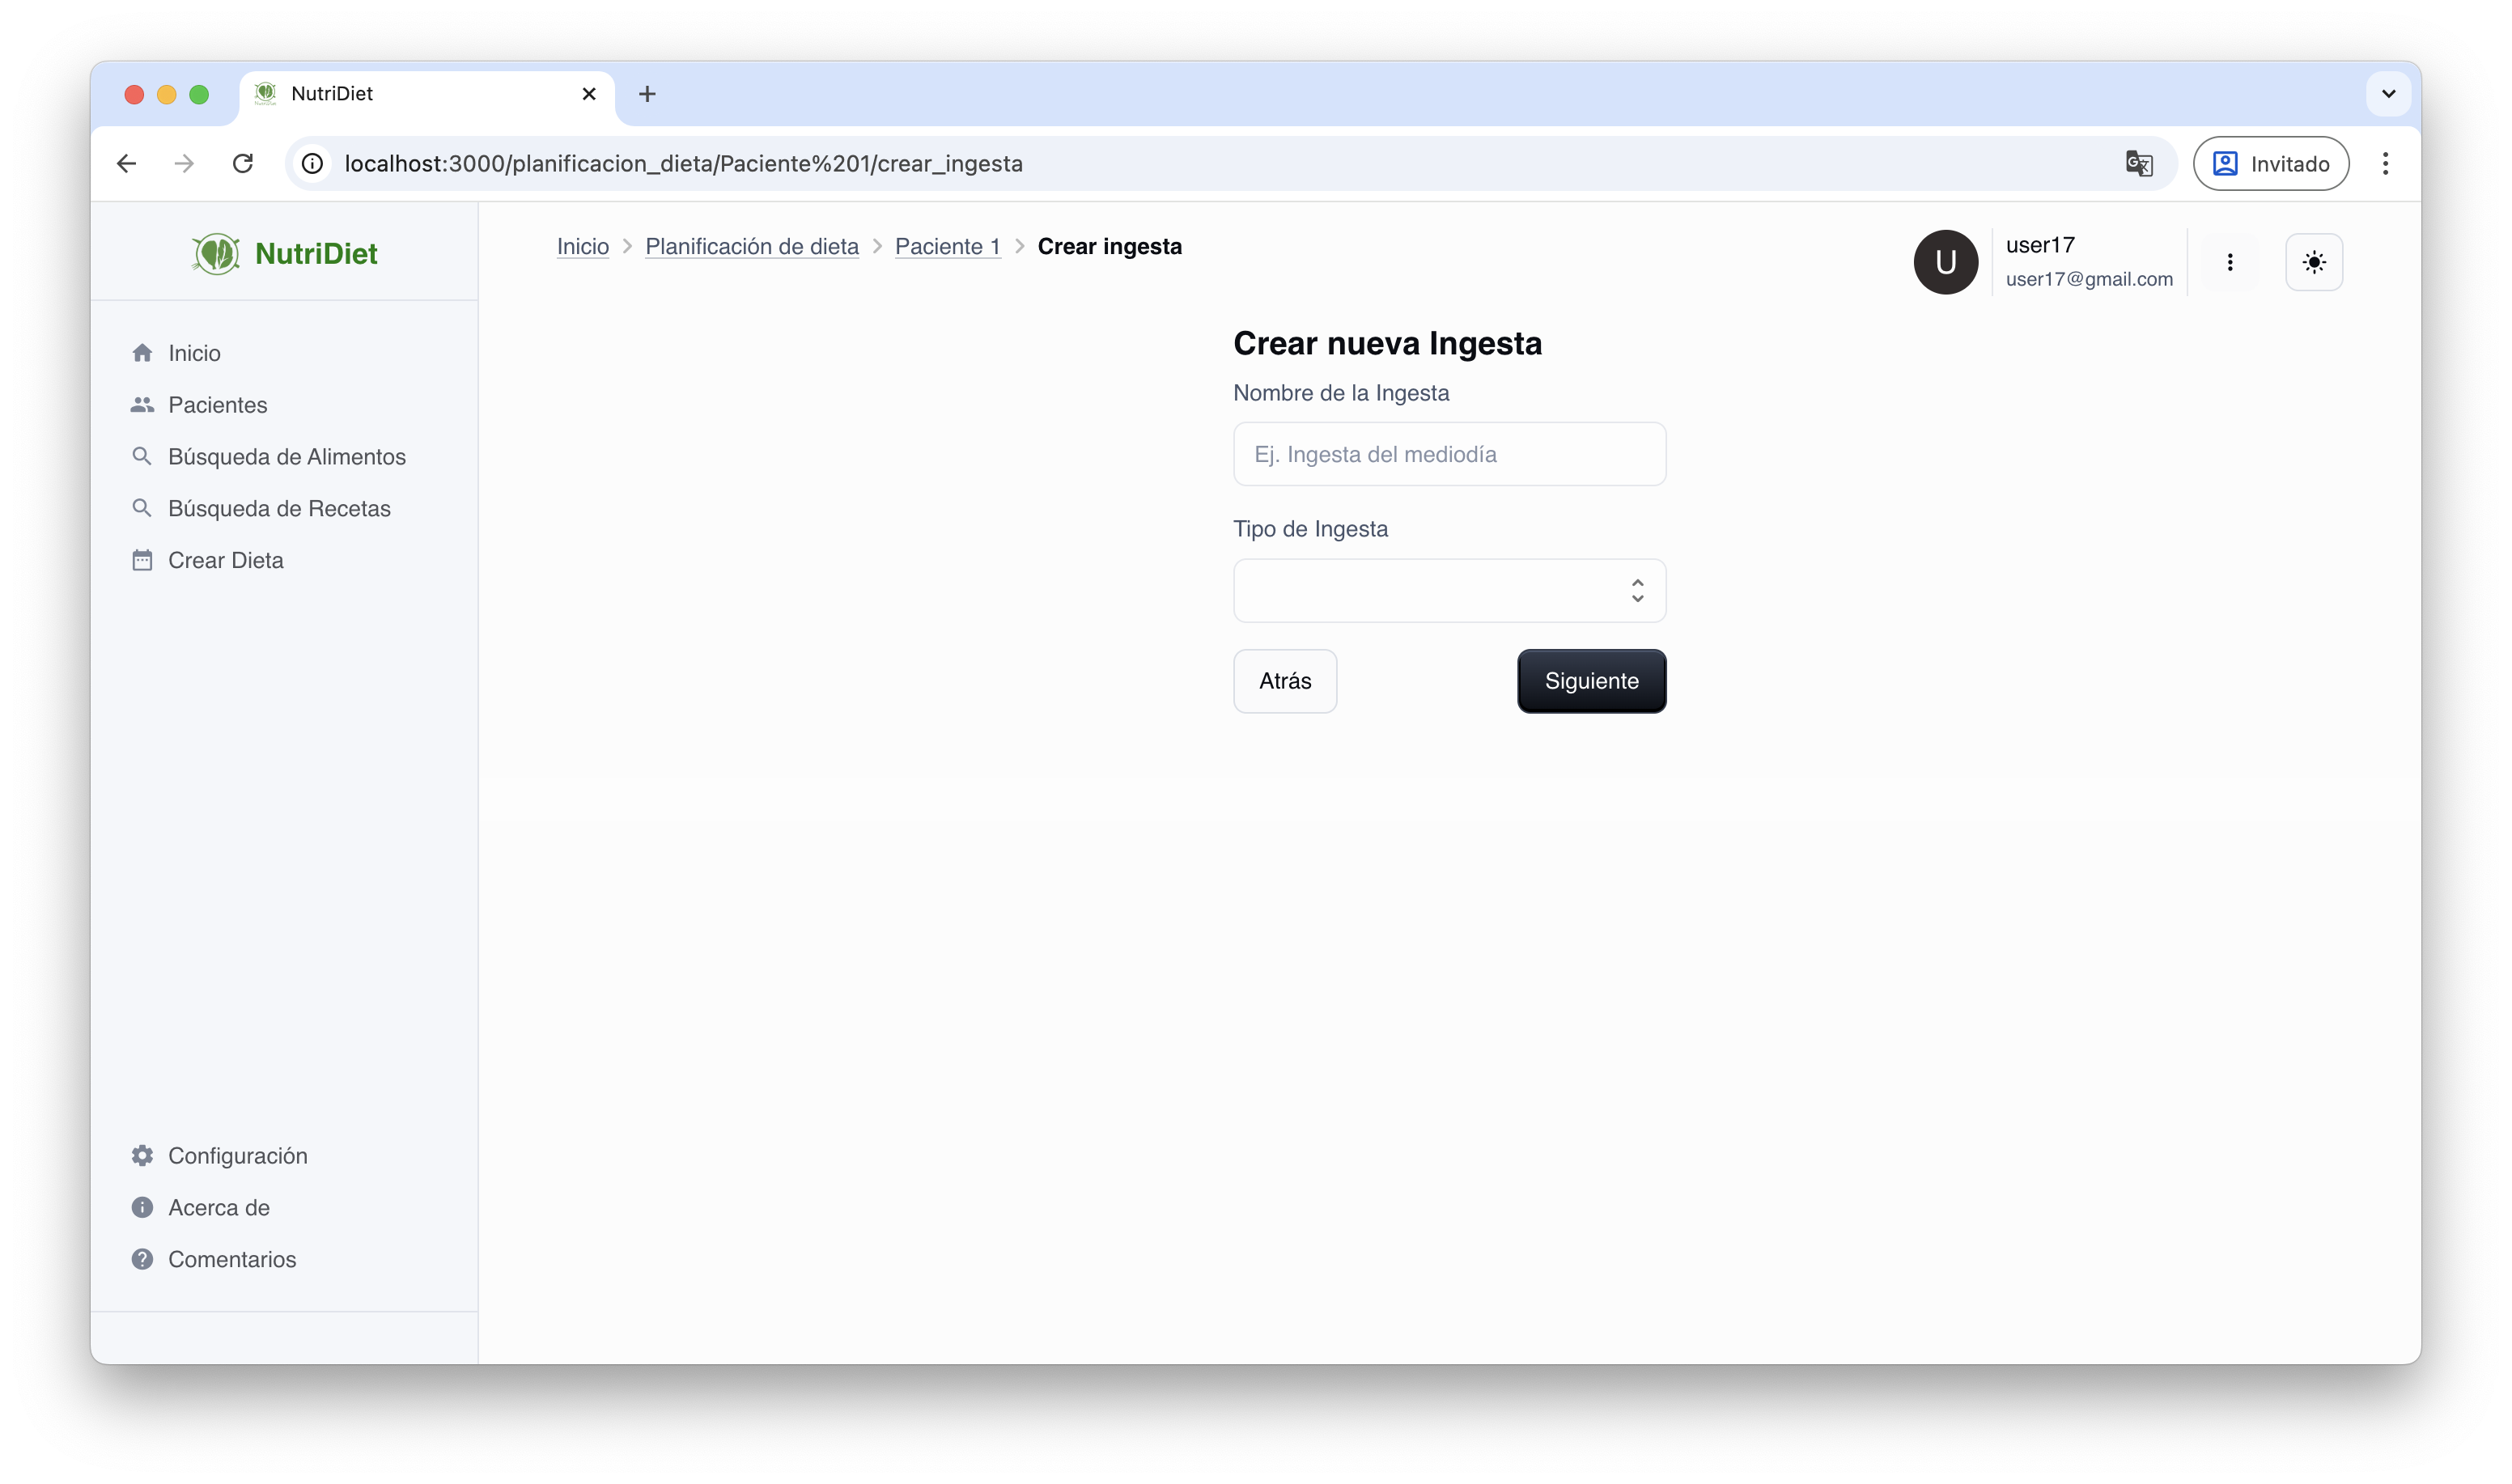
\includegraphics[width=1\linewidth]{Plantilla_TFG_latex/imagenes/PD_crearIngestaN.png}
    \caption{Formulario inicial de creación de una nueva ingesta: nombre y tipo de comida.}
    \label{fig:crear-ingesta-form}
\end{figure}

Una vez seleccionado el tipo de ingesta, el sistema muestra de forma visual (Figura~\ref{fig:crear-ingesta-drag}) los requerimientos nutricionales diarios esperados para dicha comida, calculados en función del total diario recomendado al paciente. Estos valores incluyen calorías, proteínas y carbohidratos estimados como objetivo para esa fracción del día.

Junto al nombre de la ingesta y los valores absolutos de referencia, se presenta un panel comparativo que muestra cuánto se ha cubierto con las recetas seleccionadas. Este panel utiliza indicadores circulares que reflejan el porcentaje alcanzado de cada macronutriente respecto al objetivo marcado.

\begin{itemize}
    \item Nombre de la ingesta: aparece destacado en la parte superior del panel.
    \item Objetivo nutricional: se indican los valores en kilocalorías, gramos de proteína y carbohidratos que deberían alcanzarse según el tipo de ingesta (por ejemplo, un 30\% del total diario en un almuerzo).
    \item Porcentaje alcanzado: mediante gráficos circulares, se visualiza el progreso real conforme se añaden recetas, lo que ayuda a equilibrar la composición nutricional de la ingesta.
\end{itemize}

Esta funcionalidad permite al profesional tener una visión inmediata del grado de adecuación de la ingesta a los requerimientos establecidos, facilitando ajustes antes de guardar o aplicar la planificación.

Por debajo está la interfaz interactiva basada en el sistema de ``drag-and-drop'', donde el usuario puede buscar recetas por nombre o por categoría y arrastrarlas directamente a las zonas correspondientes según el tipo de plato. Esta organización por zonas facilita la estructuración lógica del menú. La búsqueda de recetas también permite aplicar filtros nutricionales como calorías, proteínas y carbohidratos, lo que permite crear ingestas adaptadas a diferentes objetivos dietéticos.

Cada bloque de tipo de plato puede contener una o varias recetas, y el sistema muestra visualmente cuántas se han asignado a cada uno. Además, existe la opción de marcar una ingesta como ``universal'', lo cual indica que puede ser reutilizada para diferentes pacientes.

Una vez completada la planificación, el usuario puede guardar la ingesta, la cual queda registrada y disponible para su uso posterior dentro del sistema de planificación de dietas.

\begin{figure}[t]
    \centering
    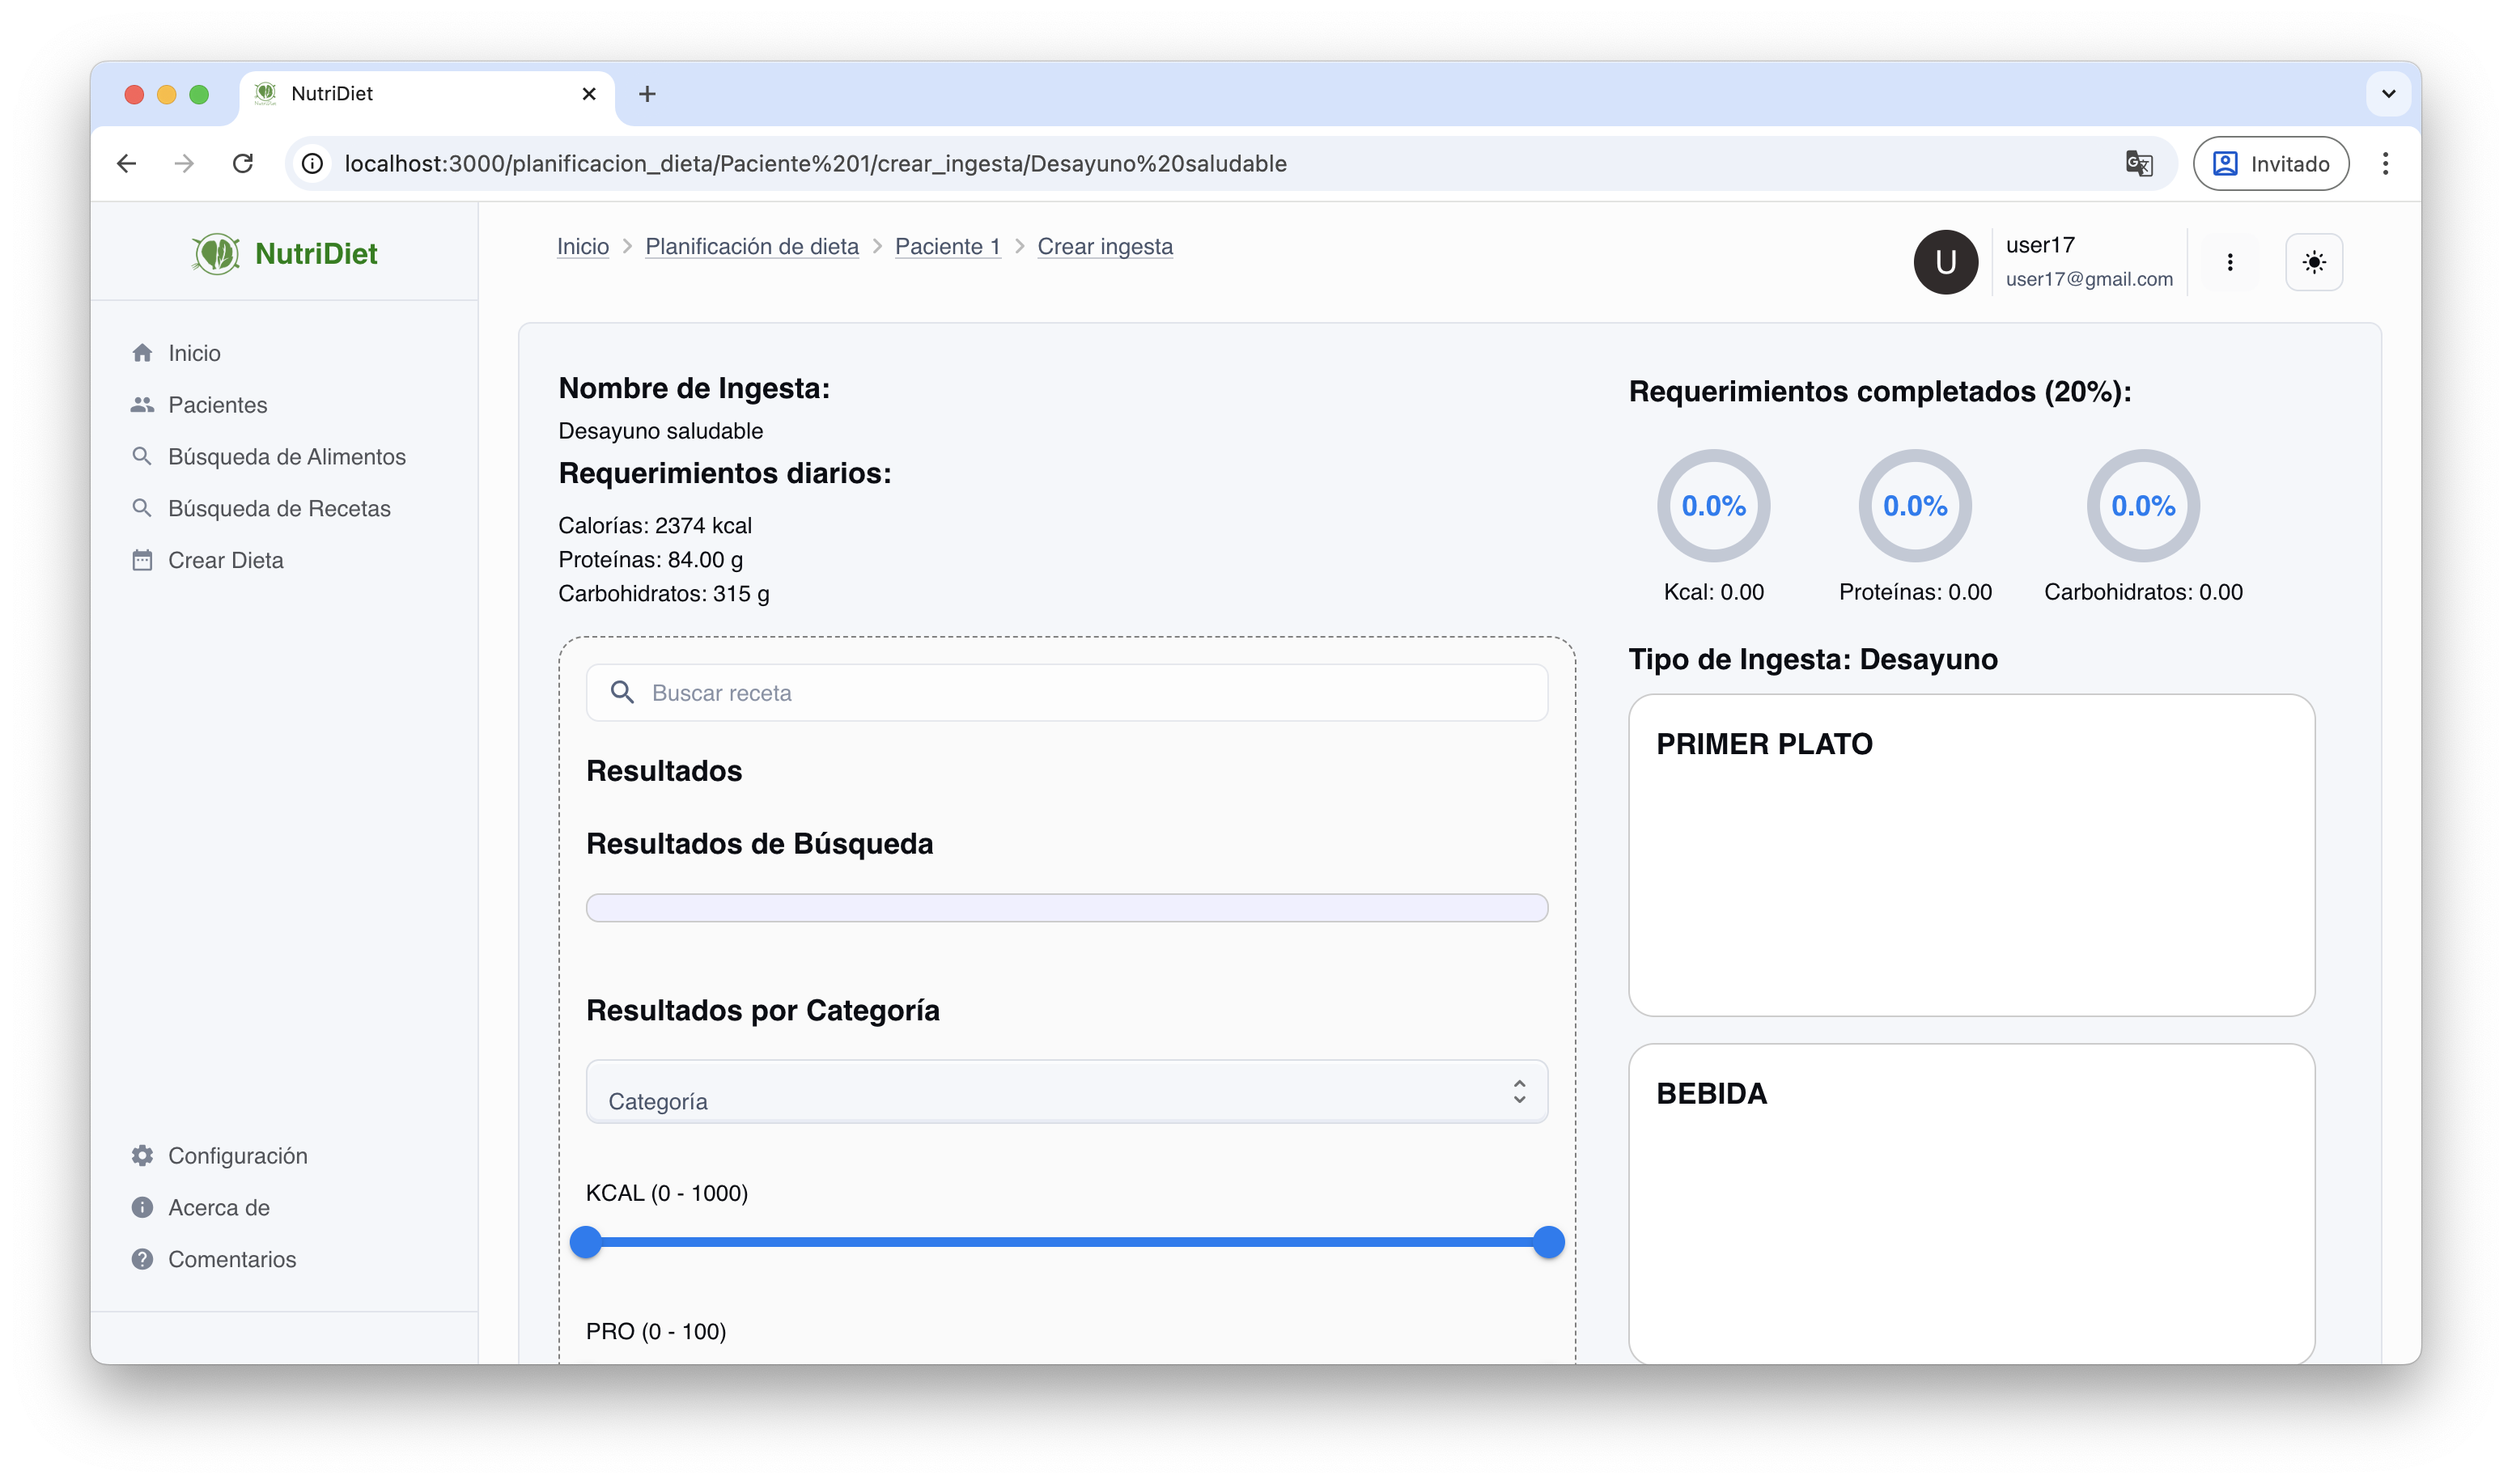
\includegraphics[width=1\linewidth]{Plantilla_TFG_latex//imagenes/PD_crearIngesta.png}
    \caption{Vista de arrastre de recetas a los bloques correspondientes por tipo de plato con requerimiento de nutrición esencial.}
    \label{fig:crear-ingesta-drag}
\end{figure}

\subsection{Crear dieta}
La creación de una dieta permite al profesional definir un plan nutricional estructurado para un paciente durante un intervalo de fechas concreto. 
Cada día del plan puede incluir una o varias ingestas ya existentes, o nuevas que se crean en el momento, asegurando así una planificación flexible y personalizada.

El proceso de creación comienza con la selección de un rango de fechas (Figura~\ref{fig:crear-dieta-form}). Una vez definido el periodo de planificación, el sistema muestra los requerimientos nutricionales diarios del paciente (calorías, proteínas, carbohidratos), como referencia para evaluar si la dieta está balanceada globalmente.

\begin{figure}
    \centering
    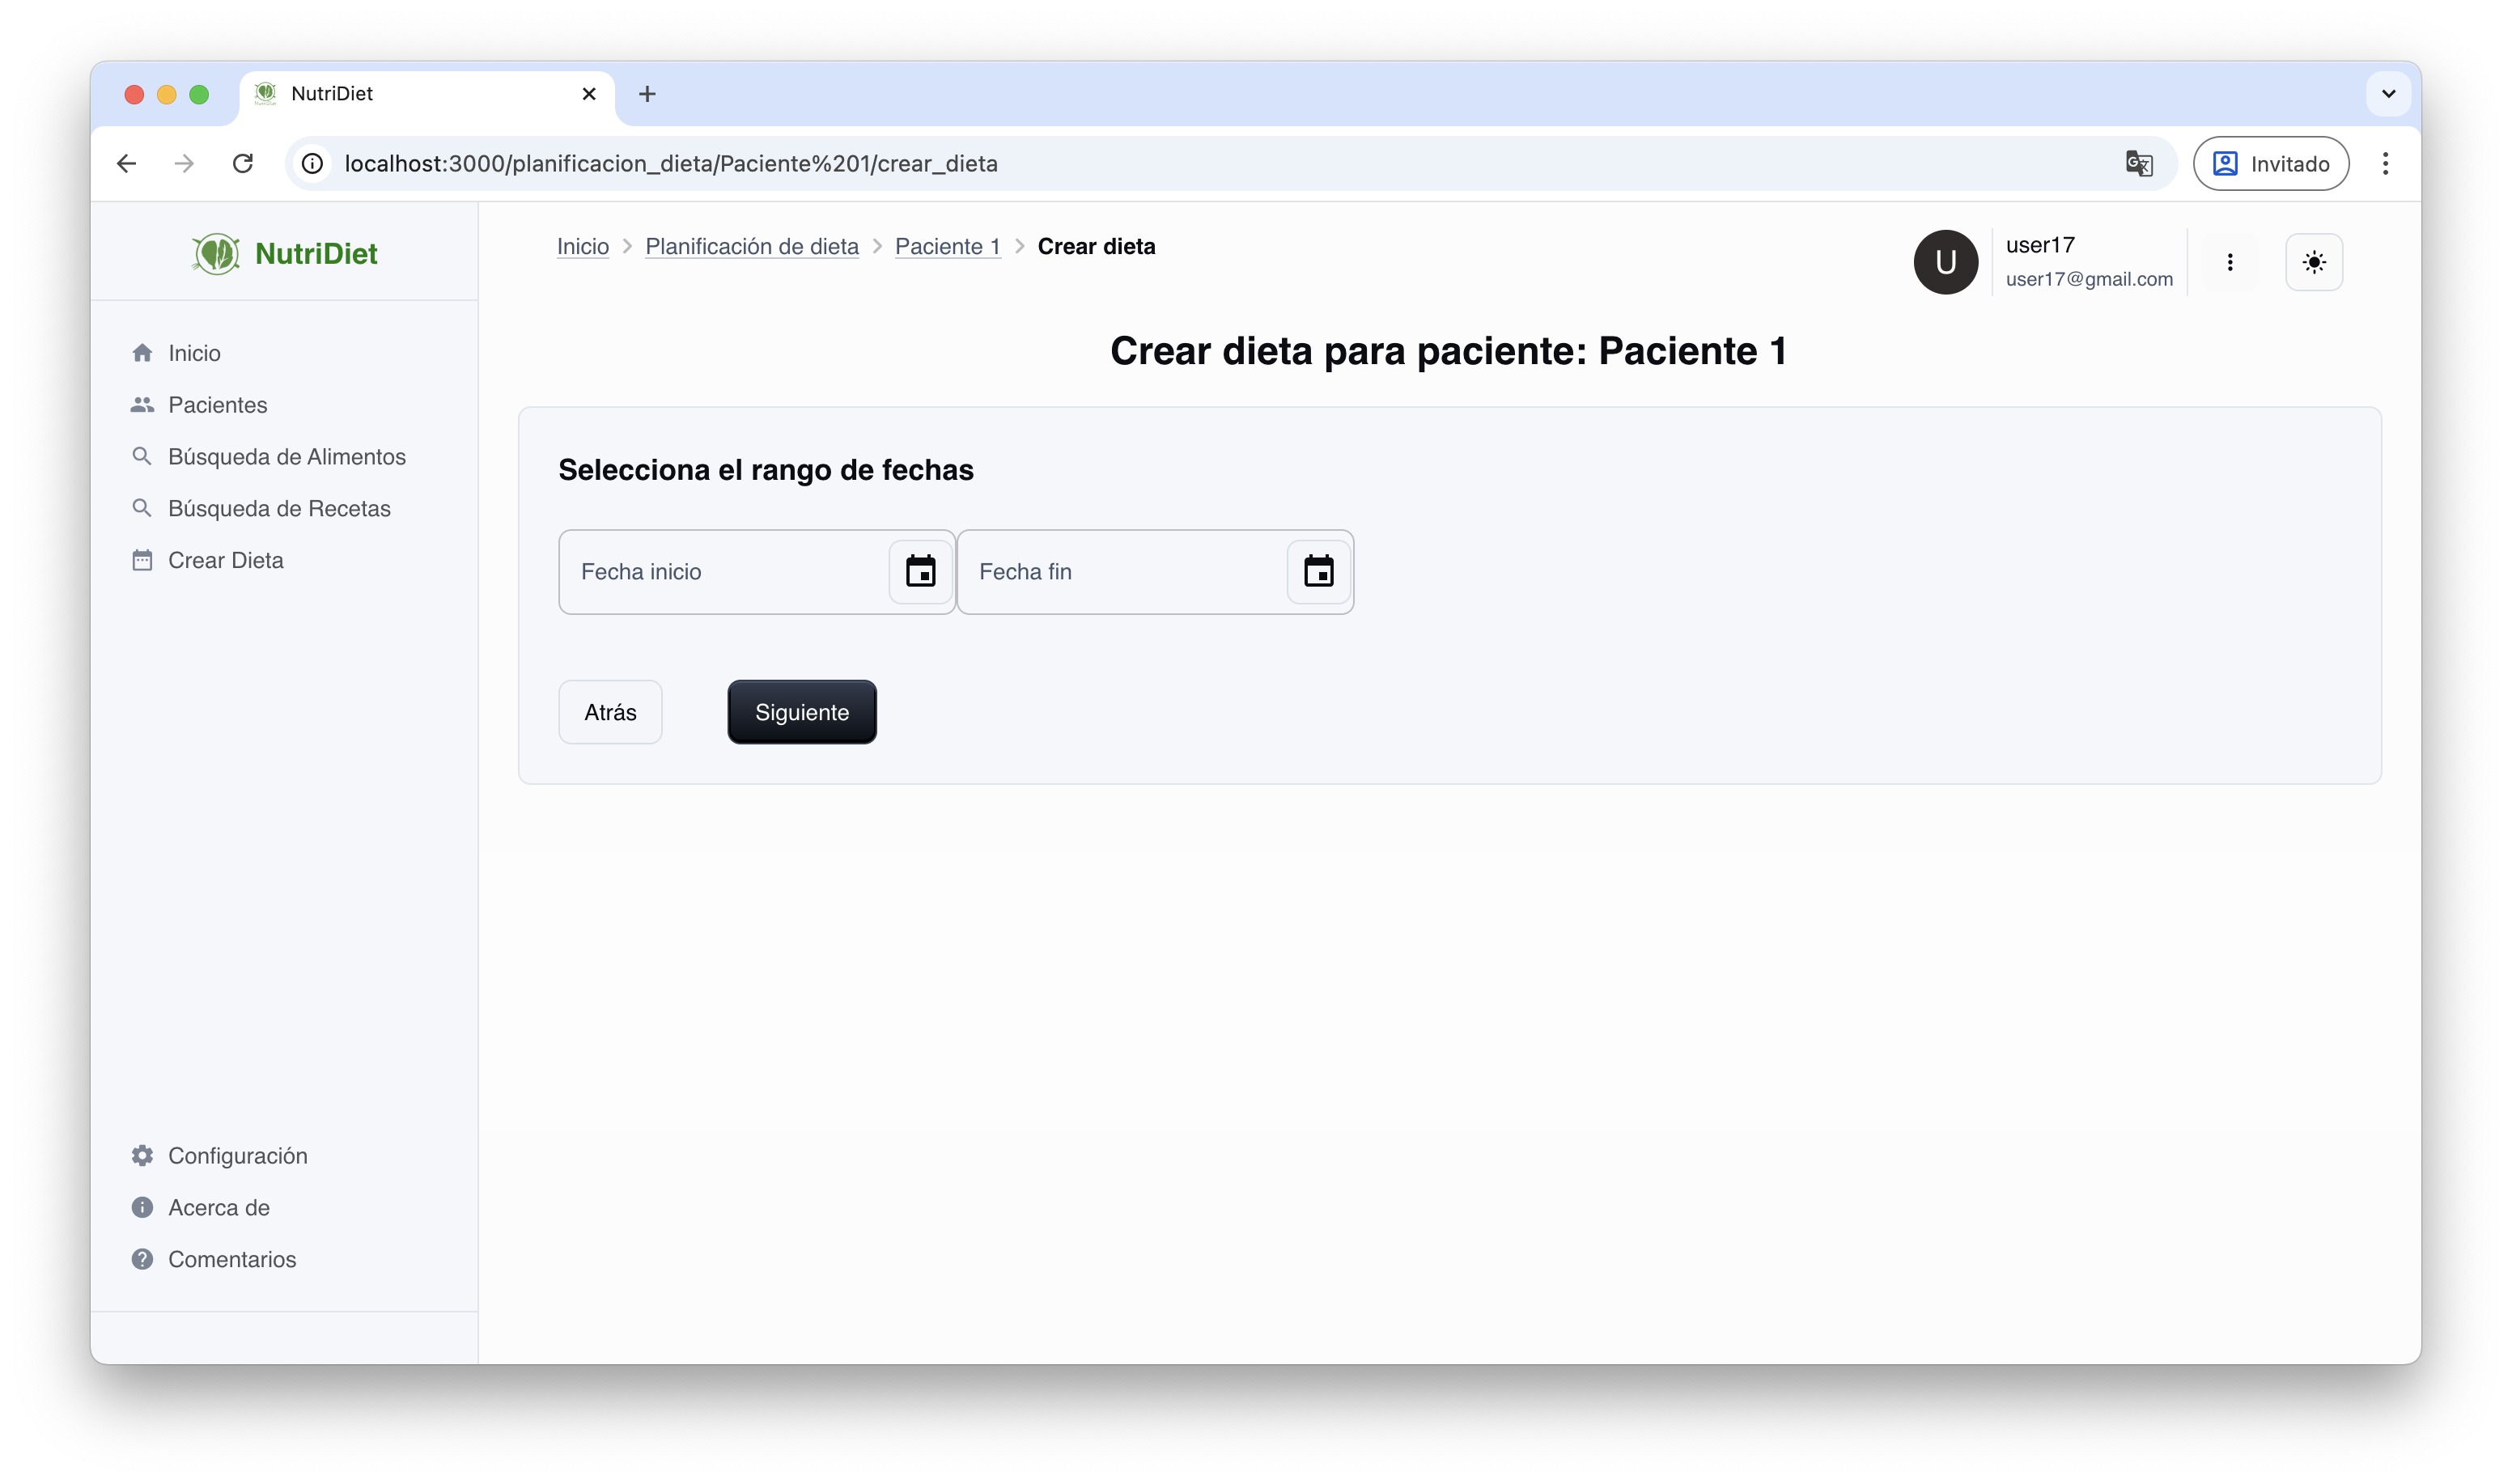
\includegraphics[width=1\linewidth]{Plantilla_TFG_latex//imagenes/PD_creardieta.png}
    \caption{Formulario inicial para crear una nueva dieta: selección de fechas.}
    \label{fig:crear-dieta-form}
\end{figure}

La interfaz (Figura~\ref{fig:crear-dieta-plan}) se compone de dos secciones principales:

\begin{figure}
    \centering
    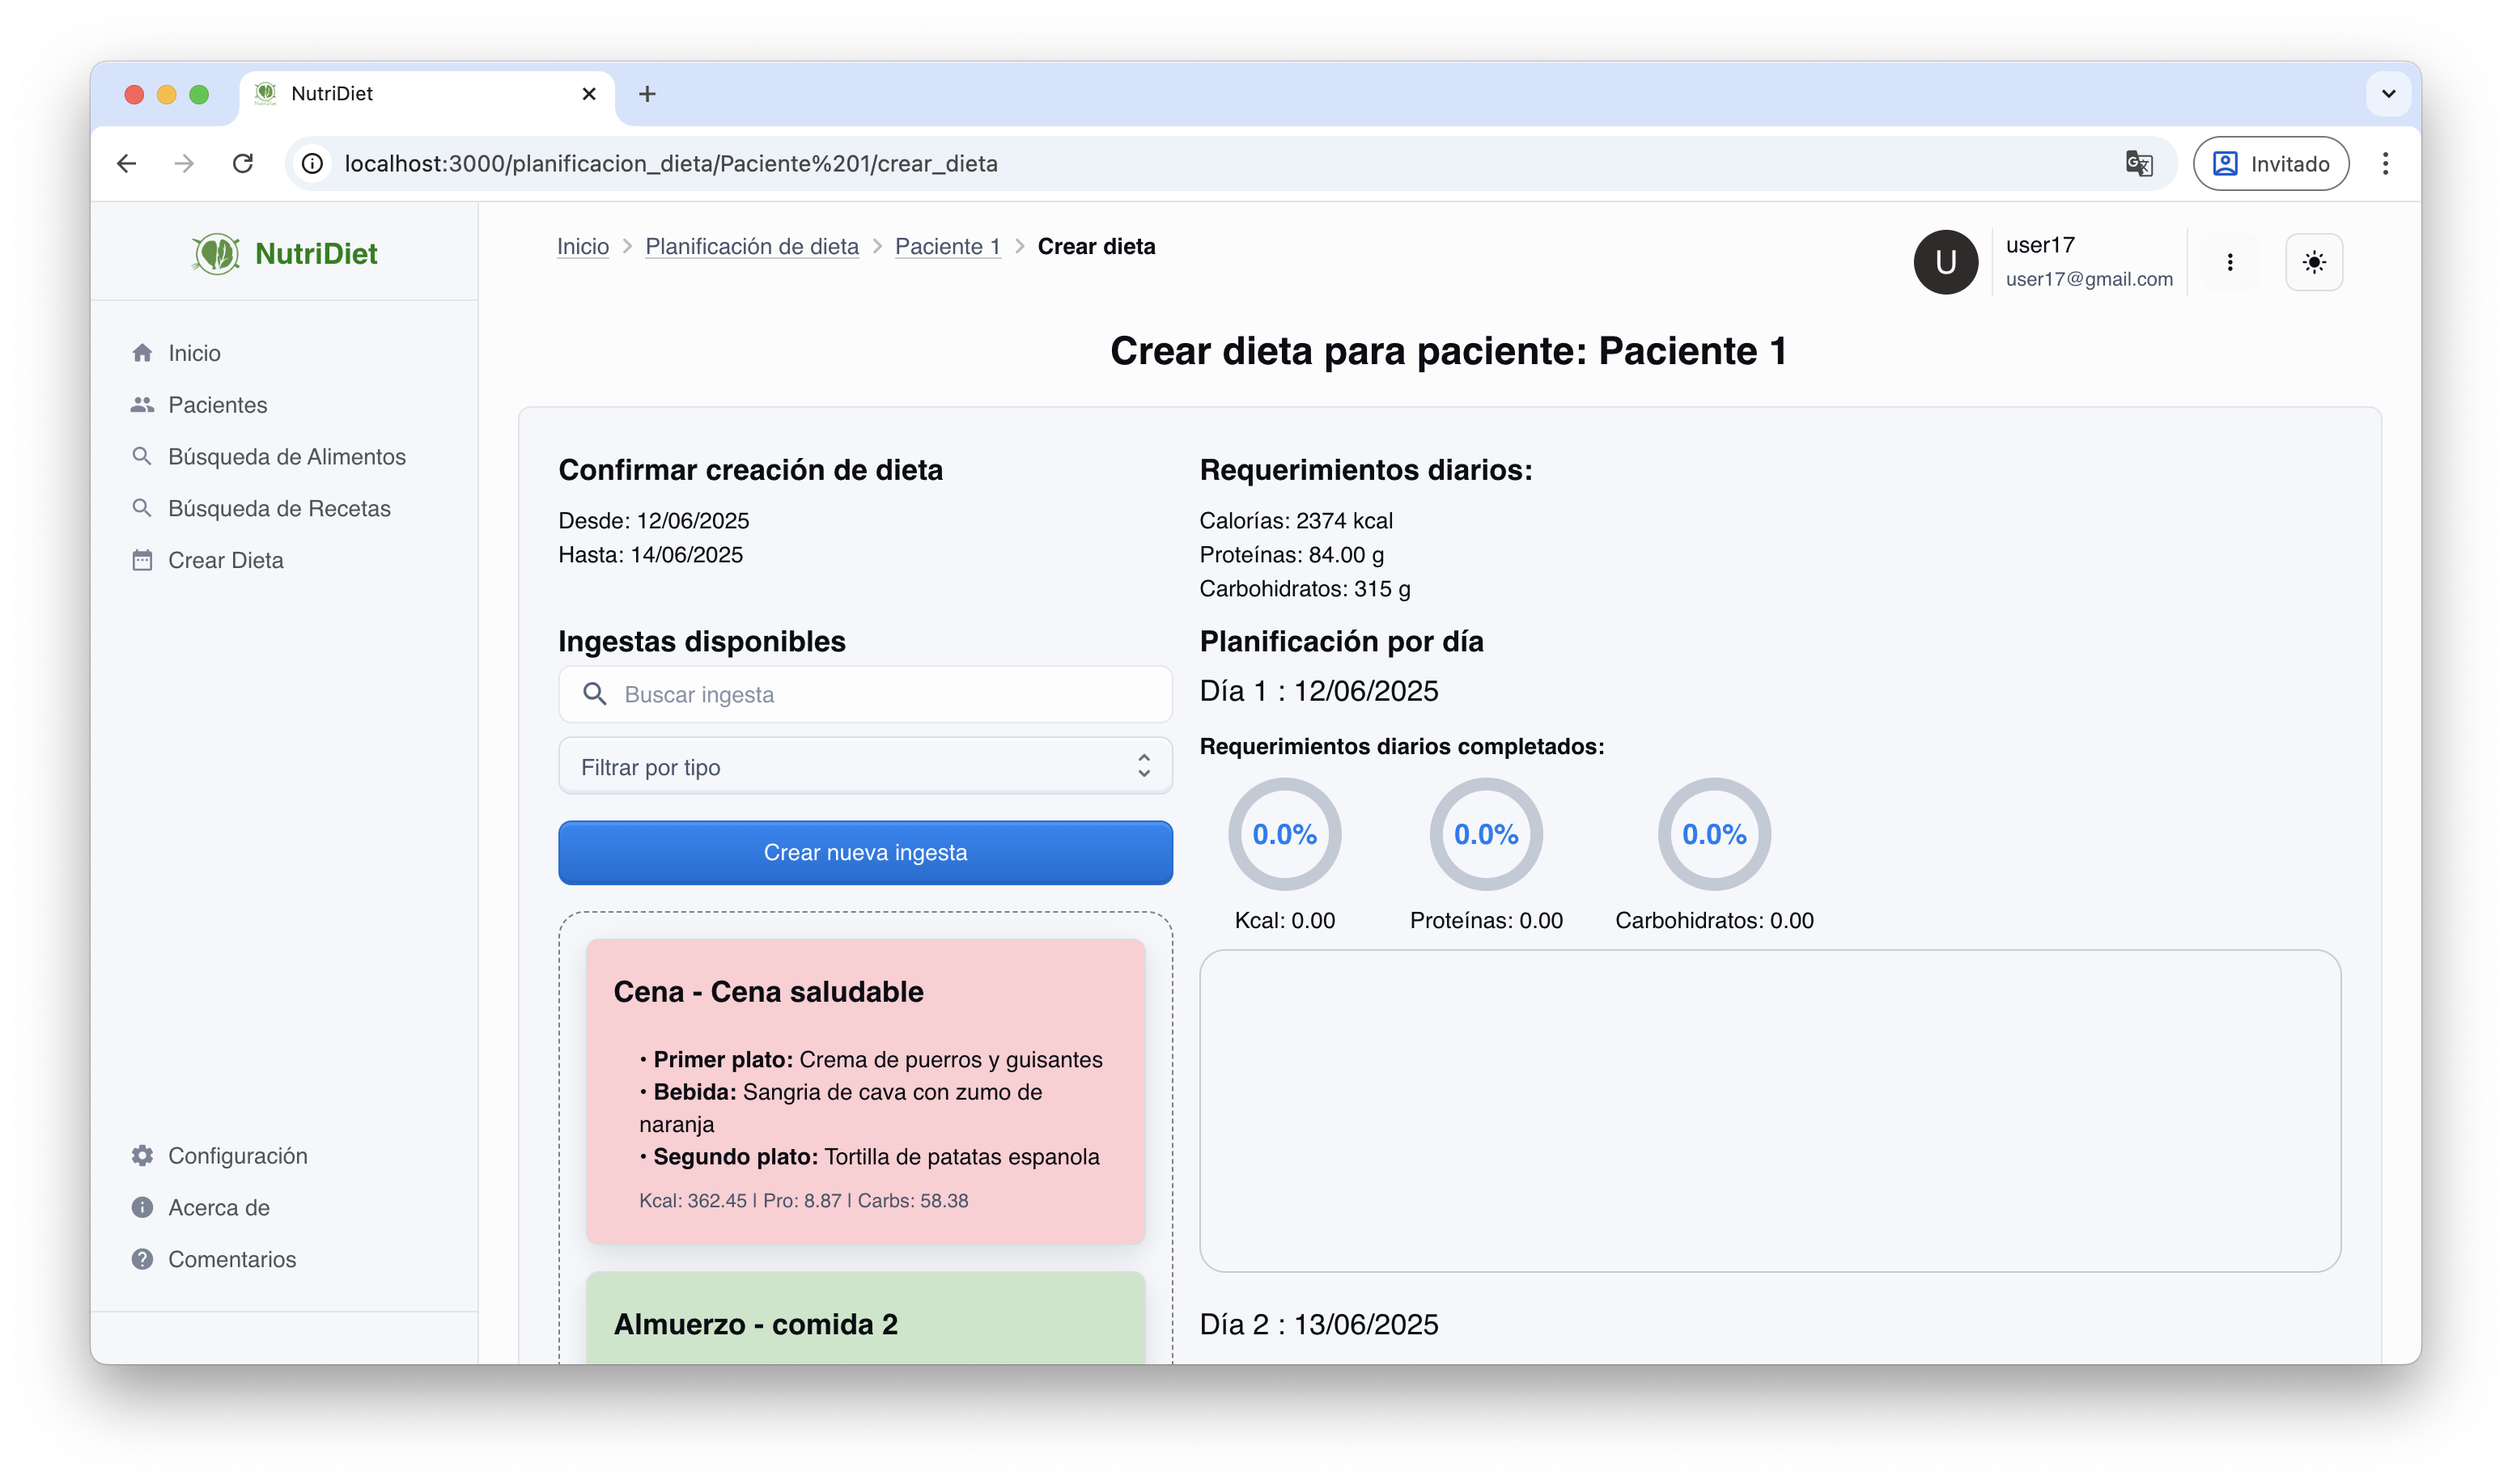
\includegraphics[width=1\linewidth]{Plantilla_TFG_latex//imagenes/PD_crearDietas.png}
    \caption{Vista de planificación de dieta diaria mediante ``drag-and-drop'' de ingestas, con seguimiento nutricional por día.}
    \label{fig:crear-dieta-plan}
\end{figure}

\begin{itemize}
    \item Ingestas disponibles: un panel lateral con buscador y filtros por tipo de ingesta (desayuno, almuerzo, cena, etc.), que permite seleccionar o crear nuevas ingestas. Cada ingesta está representada como una tarjeta informativa que incluye sus recetas y su valor nutricional total.

    \item Planificación por día: una vista desplegable por día, que muestra el nombre, las ingestas asignadas, y un resumen visual de los requerimientos cubiertos. El usuario puede arrastrar y soltar (``drag-and-drop'') ingestas desde el panel lateral hacia un día determinado para construir el plan nutricional.
\end{itemize}

Cada tarjeta de ingesta puede ser movida o eliminada fácilmente, y el sistema permite duplicarlas si es necesario planificar la misma comida en varios días. Para cada día, se muestra un panel de seguimiento con círculos de porcentaje que indican el grado de cumplimiento de los requerimientos nutricionales diarios con las ingestas añadidas.

Además, el sistema permite crear una nueva ingesta durante el proceso de planificación mediante un formulario en ventana modal, sin abandonar el contexto de edición de dieta. Esta funcionalidad favorece una experiencia continua y sin interrupciones.

Una vez finalizada la planificación, el profesional puede guardar la dieta, la cual queda asociada al paciente y disponible para su consulta, edición o eliminación posterior.

\section{Otras funciones del sistema}

\subsection{Configuración}
La pantalla de ``Configuración'' (Figura~\ref{fig:pantalla-configuracion}) permite personalizar aspectos visuales y funcionales del sistema según las preferencias del usuario. Actualmente se incluyen las siguientes opciones:

\begin{itemize}
    \item Modo de color: Permite elegir entre distintos temas visuales (claro u oscuro), adaptando la interfaz a la preferencia visual del usuario. Esta selección se gestiona mediante un componente personalizado.
    
    \item Orden de tarjetas: El usuario puede seleccionar el orden en que se muestran las tarjetas principales de la página de inicio (Figura~\ref{fig:pagina_inicio}), como ``Alimentos'', ``Recetas'', ``Pacientes'' o ``Dietas''. Esta preferencia se guarda localmente en el navegador utilizando ``localStorage'', lo que asegura que se mantenga incluso tras cerrar la sesión.
\end{itemize}

\begin{figure}[t]
    \centering
    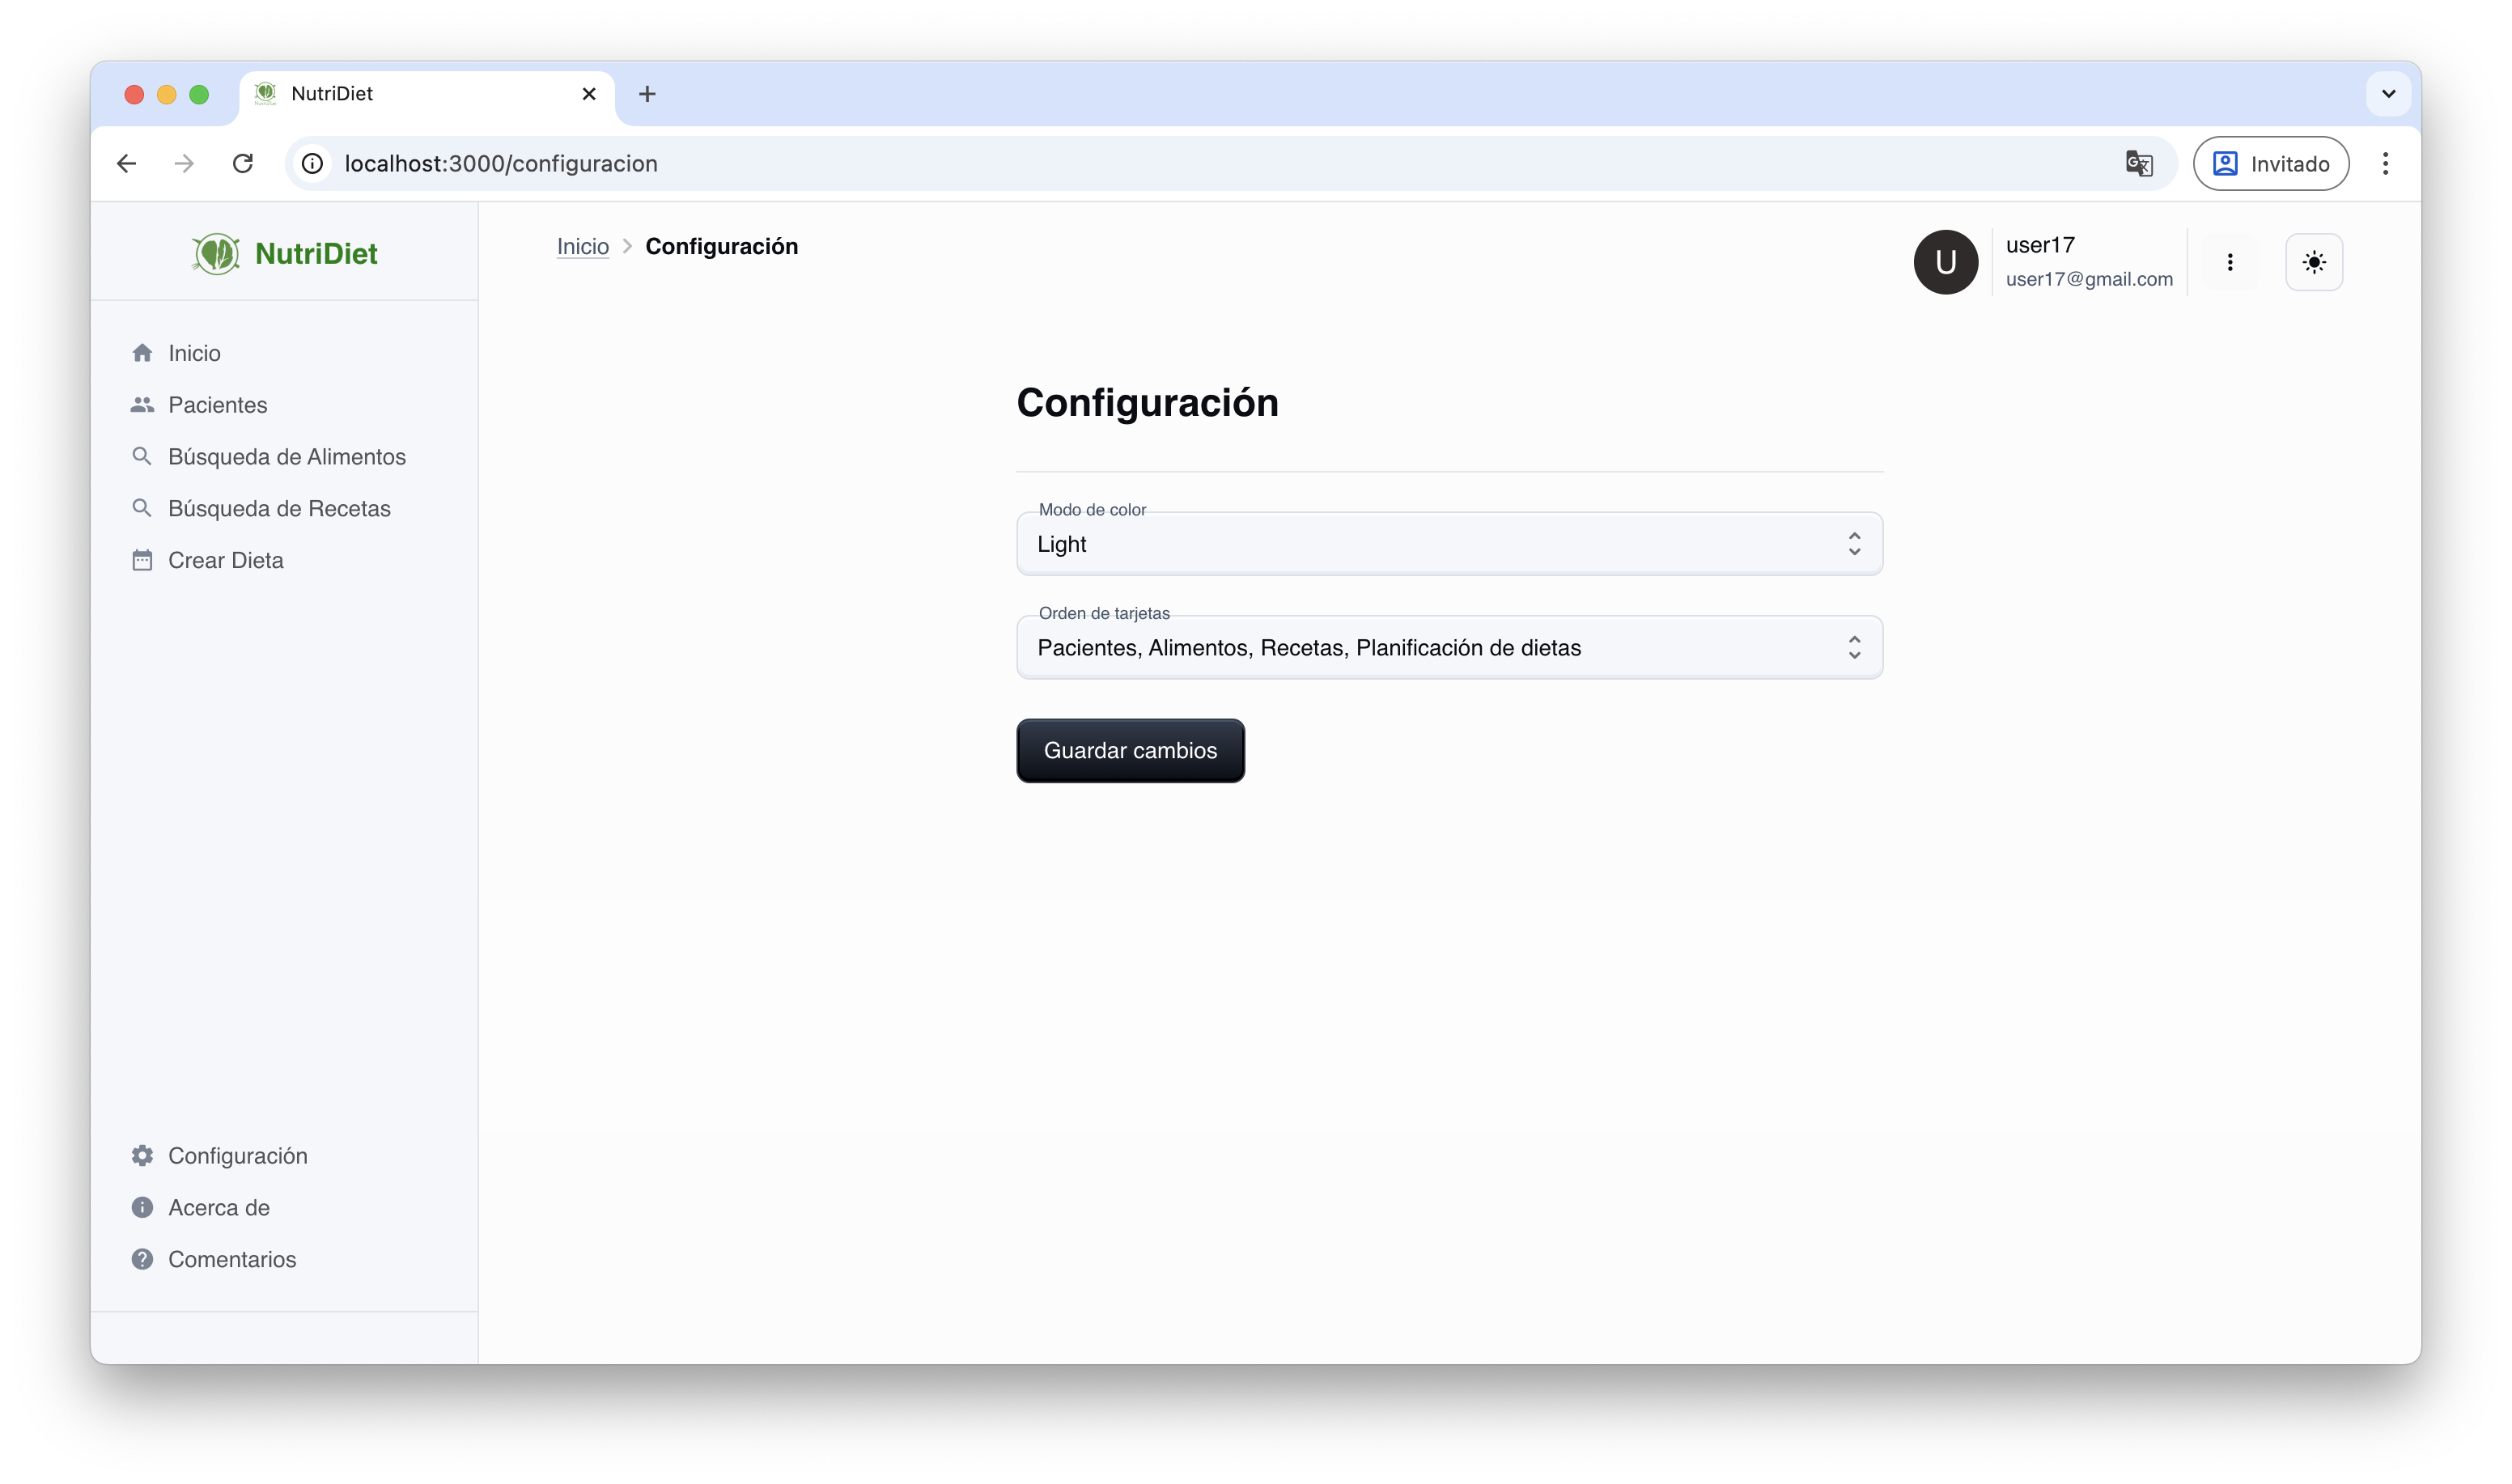
\includegraphics[width=1\linewidth]{Plantilla_TFG_latex//imagenes/Configuracion.png}
    \caption{Pantalla de configuración del sistema}
    \label{fig:pantalla-configuracion}
\end{figure}

\section{Consideraciones finales del capítulo}
En este capítulo proporciona una guía detallada sobre el funcionamiento de cada una de las funcionalidades integradas en el sistema.
Cada módulo ha sido diseñado con un enfoque centrado en la usabilidad y la personalización, como se refleja en opciones como la configuración del sistema o la planificación alimentaria adaptada a cada paciente. 

En conjunto, el sistema cumple con los requisitos establecidos y responde de manera efectiva a las necesidades detectadas durante el análisis, consolidándose como una solución digital integral para la gestión nutricional personalizada. Además, se ha realizado un video de demo funcional donde se puede visualizar el comportamiento del sistema (\url{https://drive.google.com/file/d/10IC1oFVbOKyTe_VdsKLkdpSt9aNQeZIn/view?usp=sharing}).
